\documentclass[twoside,openany]{SDUthesis}
%\hypersetup{colorlinks=false}
%\makeatletter
%\renewcommand\normalsize{%
%   \@setfontsize\normalsize\@xpt\@xiipt
%   \abovedisplayskip 6\p@ \@plus3\p@ \@minus4\p@
%   \abovedisplayshortskip \z@ \@plus3\p@
%   \belowdisplayshortskip 6\p@ \@plus3\p@ \@minus3\p@
%   \belowdisplayskip \abovedisplayskip
%   \let\@listi\@listI}
%\makeatother

\newcommand{\makeheadrule}{%ҳü
\makebox[0pt][l]{\rule[0.55\baselineskip]{\headwidth}{0.3pt}}
\rule[0.7\baselineskip]{\headwidth}{2.5pt}}
\renewcommand{\headrule}{%
{\if@fancyplain\let\headrulewidth\plainheadrulewidth\fi
\makeheadrule}}
\makeatother

\makeatletter
\newcommand{\figcaption}{\def\@captype{figure}\caption}
\newcommand{\tabcaption}{\def\@captype{table}\caption}
\makeatother

\setlength{\abovecaptionskip}{0pt}
\setlength{\belowcaptionskip}{0pt}

\usepackage{mathrsfs}
\usepackage{pdfpages}
\usepackage{changepage}

%\usepackage{subfigure}
\usepackage{color}
\usepackage{ulem}
\usepackage{graphicx}
\usepackage{subfig}
\usepackage{longtable}
\usepackage{epstopdf}
\usepackage{ccmap}
%\newcommand{\tabincell}[2]{\begin{tabular}{@{}#1@{}}#2\end{tabular}}
%\newcommand{\upcite}[1]{\textsuperscript{\textsuperscript{\cite{#1}}}}

\begin{document}
\raggedbottom

\includepdfmerge{FrontReviewTwo-LCX.pdf,-}

%\makeOSandCPRTpage


\SDUfrontmatter

\SDUcontents
\SDUEcontents

%%%%%%%%%%%%%%%%%%%%%%%%%%%%%%
%% abstract
%%%%%%%%%%%%%%%%%%%%%%%%%%%%%%
\begin{abstract}
\eabstract{Abstract in Chinese}

������ӭ����Ϣ��ը��ʱ���������������������Ƽ��㼰�ƶ��罻ý�����Ϣ������Ѹ�ٷ�չʹ�����ݵ������͹�ģ�������ӣ������ʹ��ģ�����ݶ����ݵĴ����ٶȼ��洢�������涼�и��ߵ����󣬲���Ҫ�ڿɽ���ʱ���ڴ������ģ���ݣ�ͬʱ���ݵĴ洢����ҲҪ�����ڿɳ��ܷ�Χ�ڣ�����ڵ�ǰ���ģ��ģ̬���ݵļ�����Ȼ��һ����ս��Ϊ�˽����ά���ģ���ݵĽ�������ڼ������⣬���ڹ�ϣ�Ľ�������ڼ�������Ӧ�˶�������ϣ������ԭʼ�����ó��ȹ̶��Ķ�ֵ��ϣ������ʾ����ʹ��ԭʼ�����ռ��е������ϵ����������Ϣ�ں����ռ������ɱ��֡�

�������ͳ�Ĺ�ϣ������Ҫ��Ե�ģ̬���ݣ�������ǵ���ģ̬�ڵ����ݼ������⣬��������Ϣ�����Ŀ��ٷ�չ�������ݵı�ը����������ģ̬����Խ��Խ�࣬�����ڶ��ģ̬֮������ݼ������󳡾�Ҳ�������࣬��������ͼ�ȣ���˿�ģ̬��ϣ������Ϊһ����֮��Ч�Ľ��������

Ŀǰ�Ѿ������˶��ֻ��ڻ���ѧϰ�Ŀ�ģ̬��ϣ��������ȡ���˲����ļ���Ч�����������м������������ܵ�������ڣ�1) ���ڶ�ֵ��ɢ�Ż�������ѽ����һЩ��������ɢ���������ɳڣ����������ϣ���ʵֵ��ʾ��֮��Եõ���ʵֵ��ʾ���ж�ֵ���õ����յĹ�ϣ�룬Ȼ�������ɳ��Ż���ʽ������ϴ��������ʹ�����չ�ϣ��ļ���Ч���½���2) ��ǰҲ��һЩ����ֱ�ӽ�����ɢ�Ż�������������ѵ��ʱ��Ϊ���ۣ������Ż�����ʱ�������ӣ�3) �ڼල��Ϣ��ѡ���ϣ��еķ���ѡ��ʹ��\ $n \times n$ �������Ծ�����������Ա��֣�����ᵼ����ѵ����ʱ�临�Ӷȴ�����$O(n)$������$O(n^2)$����������������չ�����ģ���ݼ����Ѷȡ�

�ۺϿ�����������֮�󣬱������һ���мල��ϣ�����������ھ���ֽ�Ŀ���չ��ɢ��ϣ�����Ϊ\ SCRATCH���÷�����Ͼ���ֽ��Լ���ǩǶ������������Ա��ֺͿ���չ�����⣬�������������ת�����������Ż������й�ϣ�����ɢ���ԣ��Ӷ��ɿ��ٵ����ģ��ѵ���������������ȡ�������Ҫ�����ܽ����£�

\begin{itemize}
\vspace{-3mm}
\item ���һ��ȫ�µĻ��ھ���ֽ���мල��ģ̬��ϣ������ͨ������Эͬ����ֽ⣨CMF���ͱ�ǩ����Ƕ�룬\ SCRATCH �ɳ���������еļල������Ϣ���ҵ�һ�������ӿռ䣬ʹ����̬���������֮���������������ܹ�����Ч�ز�׽�����Ӷ������ܵı���ģ̬���ģ̬�ڵ����������ԡ�
\vspace{-3mm}
\item \ SCRATCH ʹ�ñ�ǩ������������Ծ��������ѵ����ʱ�ո��Ӷ�ʼ�������ݼ���ģ����Ϊ���Թ�ϵ���ɷ������չ�����ģ��ģ̬���ݼ��ϡ�
\vspace{-3mm}
\item Ϊ�˱���ʹ���ɳڼ��������ɢ�Ż�������ɵľ޴�������\ SCRATCH �������������ת����ʹ��ѵ��������ʼ�ձ��ֹ�ϣ�����ɢ���ԣ�����ϵ����Ż��IJ��ԣ��Ӷ���С��ѵ�������е���������������ʹ�õ��Ǿ����Ż�����������Ľ����ͨ���󵼵ó����ʽ�⣬��˱�����������ɢ�Ż�����������ѵ��ʱ��Ϊ���۵����⡣
\vspace{-3mm}
\item ͨ����������ģ̬���ݼ��Ͻ��жԱ�ʵ�飬�����������ܡ�ѵ��ʱ���Լ�ʹ�����������ȡͼ��ģ̬�������\ SCRATCH ����ʧ�������뵱ǰ�Ƚ�����ȿ�ģ̬��ϣ�����������ܶԱȣ����Կ������ķ����ڸ���ָ���ϴﵽ��ǰ׿Խ�����ܵ�ͬʱ��ѵ��ʱ���󽵵ͣ��Ӷ����Է������չ�����ģ���ݼ��ϣ����м��ߵ���Ч�Ժ�ʵ���ԡ�
\end{itemize}


\noindent\textbf{�ؼ��ʣ�}��ϣѧϰ����ģ̬����������ֽ⣻��ɢ�Ż�����������ڼ���
%\vspace{0.5em}
%\begin{tabular*}{\textwidth}{ll}
%\hspace{-1em}
%\textbf{�ؼ��ʣ�}& �Ǿֲ������ԣ�ϡ���ԣ�ͼ��ȥ�룻\\
%                &ͼ��ƽ����
%\end{tabular*}
\end{abstract}


%%%%%%%%%%%%%%%%%%%%%%%%%%%%%%
%% english abstract
%%%%%%%%%%%%%%%%%%%%%%%%%%%%%%
\begin{englishabstract}
\eabstract{Abstract in English}

Recent years have witnessed the era of information explosion, in which the rapid development of information technology, i.e., Internet, e-commerce, cloud computing and mobile social media, has led to a sharp increase in the number and size of data. Large-scale multi-modal data put forward higher requirements on data processing and storage capacity, which is not only to process large-scale data in an acceptable time, but also limit the storage capacity of data to an acceptable range. This is still a challenge for the retrieval of large-scale multi-modal data. Hashing emerges in order to solve the problem of approximate nearest neighbor retrieval for high-dimensional large-scale data. It represents the original data  as a fixed-length binary hash code and maintain the original similarity information such as semantic relations in Hamming space.

Most of the traditional hashing methods are mainly designed for single-modal data, which solves the problem of data retrieval in a single modality. With the rapid evolution of information technology and the explosive growth of data, multi-modal data is increasing. Therefore, there are more requirements for cross-modal retrieval, such as using text to retrieve image, and cross-modal hashing retrieval becomes an effective solution.

At present, there are many cross-modal hashing methods based on machine learning, and have achieved great retrieval performance, but there are still some limitations on their performance: As the binary discrete optimization problem is more difficult to solve, some methods relax the discrete conditions by first obtaining the real-valued representation of the hash code, and then binarizing the obtained real-valued representation to obtain the final hash code. However, the relaxation optimization will generate a large quantization error, leading to poor retrieval performance. There are also some methods for direct discrete optimization, but the time required for optimization is greatly increased. In the choice of supervised information, some methods choose to use $n \times n$ similarity matrix for similarity maintaining, which will increase the time complexity of training from linear $O(n)$ to $O(n^2)$, making it harder to extend to large-scale datasets.

After comprehensively taking the above problems into account, this paper proposes a new supervised hashing method, namely, Scalable disCRete mATrix faCtorization Hashing, SCRATCH for short. It combines the collective matrix factorization and semantic embedding to solve the problem of similarity preserving and scalability, and leverages random orthogonal rotation matrix to keep the discrete property of hash codes in training stage, in order to train the model as fast as possible and improve the retrieval precision. The contributions of this work are summarized as follows:

\begin{itemize}
\vspace{-3mm}
\item We propose a novel matrix factorization based supervised cross-modal hashing method. By leveraging the matrix factorization and semantic embedding, SCRATCH can make full use of current supervised semantic information to find a common sub-space where the latent semantic relations among modalities of heterogeneous data can be captured and the intra- and inter-modality similarities are preserved.
\vspace{-3mm}
\item SCRATCH uses label matrix rather than $n \times n$ similarity matrix, such that its time and space complexity are always linear with the number of dataset instances, making it scalable to large-scale datasets.
\vspace{-3mm}
\item In order to avoid the large quantization error caused by using relaxation technique to solve the discrete optimization problem, SCRATCH introduces a random orthogonal rotation matrix to keep the discrete property of hash codes in the training process, and combine with an iterative optimization strategy, thus minimizing the quantization error in the training process. What's more, as it uses matrix optimization techniques, the solution of the matrices can be got by matrix derivation to obtain its closed solution, thus avoiding the large training time of other discrete optimization techniques.
\vspace{-3mm}
\item By comparing experiments on three multi-modal datasets, including retrieval performance, training time, and using a deep network as image feature extractor with loss function of SCRATCH to compare the retrieval performance with current advanced deep cross-modal hashing methods, we can see that SCRATCH achieves state-of-the-art performance on three benchmark multi-modal datasets and the training time is greatly reduced, which means that it is extremely effective and practical and can be easily extended to large-scale datasets.
\end{itemize}


%\vspace{1mm}
%\begin{tabular*}{\textwidth}{ll}
%\hspace{-2.5em}
\noindent\textbf{Keywords:} Hash learning; Cross-modal retrieval; Matrix factorization; Discrete\\
optimization; Approximate nearest neighbor search
%\end{tabular*}

\end{englishabstract}


\SDUmainmatter

%\input{./Chapters/chap0}
\chapter{\quad\quad��\quad��}
\echapter{Introduction}
\label{chap1}

\section{���������������}
\esection{Background and motivation of Research}

\subsection{�����}
\esubsection{Background of research}

��������������Ϣ�����ķ��ٷ�չ�Լ��ƶ��豸�������罻��վ����΢����Facebook��Flickr ��\ Twitter�ȣ������У�ͼ����Ƶ����Ƶ���ı��ȶ�ý�������������͹�ģ�Ϸ��������������Щ�̺��޴���Ϣ���ĺ�����ģ̬���ݣ���ģ̬��Ϣ������ע����Ҫ����������ڱ�֤�������ȵ�ǰ���£��Ӵ��ģ�Ķ�ģ̬���ݿ��п��ٵط����û�����ѯ��ģ̬��Ϣ�����ı���ͼƬ�ȣ������ڵ�ǰ�Ķ�ģ̬���ݿ���������������ά�ȸ��Լ�Ҫ����Ӧ�ٶȿ���ص㣬��˶�ģ̬���ݼ���Ŀǰ����һ���ѵ㡣

�����ģ̬���ݼ���������ֱ�ӵĽ�������Ǿ�ȷ���ڼ���������͵ķ�����K���ڷ���K Nearst Neighbors, KNN��\cite{altman1992knn}��������������������������ݿ������������������ԣ�ͨ��ʹ�þ�����������������ԣ���Ȼ���ҳ���������󣨾�����С��������������󣩵�\ K ��������Ϊ������ѡ�������ء�Ȼ������ȷ���ڼ������������ڼ��������󣬶��ڸ�ά���ģ������˵����ʵ�ã��޷��ﵽӦ��Ч����

ʵ��Ӧ���У����ƽ��ڼ�����Approximate Nearst Neighbors, ANN��\cite{Tang15Neighborhood,hinton03stochastic,wang2015facilitating,liu2016query,nie12Harvesting,Song2013Effective,luo2018fast,Wang2016luh,Yang2017dmvh}�ڶ�ģ̬���ݼ��������˹ؼ����ã��ڼ�������õ���֤��ͬʱ����Ƚ����˲�ѯ����Ӧʱ�䣬��ʵ���Ժ���Ч�Է���õ��˺ܴ�̶ȵ���������ǰ���ڽ��ƽ��ڼ����������о���Ҫ��Ϊ�������νṹ�ͻ��ڹ�ϣ������������ʵ���������ڹ�ϣ�����Ľ��ƽ��ڼ�������ʵ�����и�����ʵ���ԡ�

��ͳ�Ļ������νṹ�Ľ��ƽ��ڼ�����Ҫ˼������㻮�����ݣ����Ϲ��˴󲿷����ݣ��Ӷ����ټ���������������Ч�ʡ����д����Է�������\ KD ��\cite{bentley1975kdtree}�����\ KD ��\cite{silpa08optkdtree}��R ��\cite{guttman1984r}��Q ��\cite{finkel1974quad}����ԪͶӰ��\cite{wang2014trinary}�ȡ���\ KD ��Ϊ������ʵ���϶�Ӧ����һ����\ $k$ ά�ռ�Ļ��֣�����\ KD ��ʱ��ÿ��ʹ�ô�ֱ��������ij�ƽ������\ $k$ ά�ռ仮��Ϊ���ɸ�\ $k$ ά��������������\ KD ����ÿ�� �ڵ���һ��\ $k$ ά�����������Ӧ��������ѯʱ��ѭ��ýڵ�����ԭ��������Ҷ�ӽڵ㣬�Ӷ����ؽ��ڽ��������ռ仮���㷨������ά�Ƚϵ͵���������ڼ������Ⱥ�Ч�ʷ���ȡ�����������Ч���������ڸ�ά�ռ��лᷢ��ά�����ѣ����»������νṹ�Ľ��ƽ��ڼ����ļ������ȼ�Ч�ʴ���½���

Ϊ�˽����ά���ģ���ݵĽ��ƽ��ڼ������⣬��ϣ����\cite{wang2016linear,yang2016zero,wang2018survey,ShenFM17TMM,SongJK18PR,ZhangHW16MM,Song2014Robust,luo2018scalable,yan2016srdmh} ��������ٶȿ�洢���ĵ͵��ŵ���ܵ��㷺��ע��̽������ͼ\ \ref{hash_example} ��ʾ��ͨ����ԭʼ��ά����ӳ�䵽�����ռ��еĵ�ά�����Ʊ�ʾ����ϣ���������������Ͷ�ģ̬���ݵĴ洢���ۣ�ͬʱͨ���ں����ռ��е�������������Ч��Ҳ��������������ϣ������Ŀ�����ں����ռ��б���ԭʼ�ռ������ݵ�֮��������ԣ���ԭʼ�ռ������Ƶ��������ں����ռ���Ҳ�ᾡ�������ƣ�ԭʼ�ռ��в����Ƶ��������ں����ռ���Ҳ�ᾡ���ܲ����ƣ���˹�ϣѧϰ��Ķ����ƹ�ϣ����һ���̶����ܹ�����ԭʼ�������������н��ƽ��ڼ�������ϣ�����ľ�������Ϊ������ͨ��Ԥ���趨��Ŀ�꺯����ܽ���ѵ���õ���ϣ�����Լ��������ݿ�Ĺ�ϣ�루Ҳ����ѧ���Ĺ�ϣ�������ɣ���Ȼ����ڴ���ѯ����ʹ�ù�ϣ�������ɶ�Ӧ��ϣ��֮���ٵ��������ݿ���ͨ���������ҵ���ѯ���ݵĽ���֮�󼴿ɷ��ؼ��������

\begin{figure}[htbp]
\centering
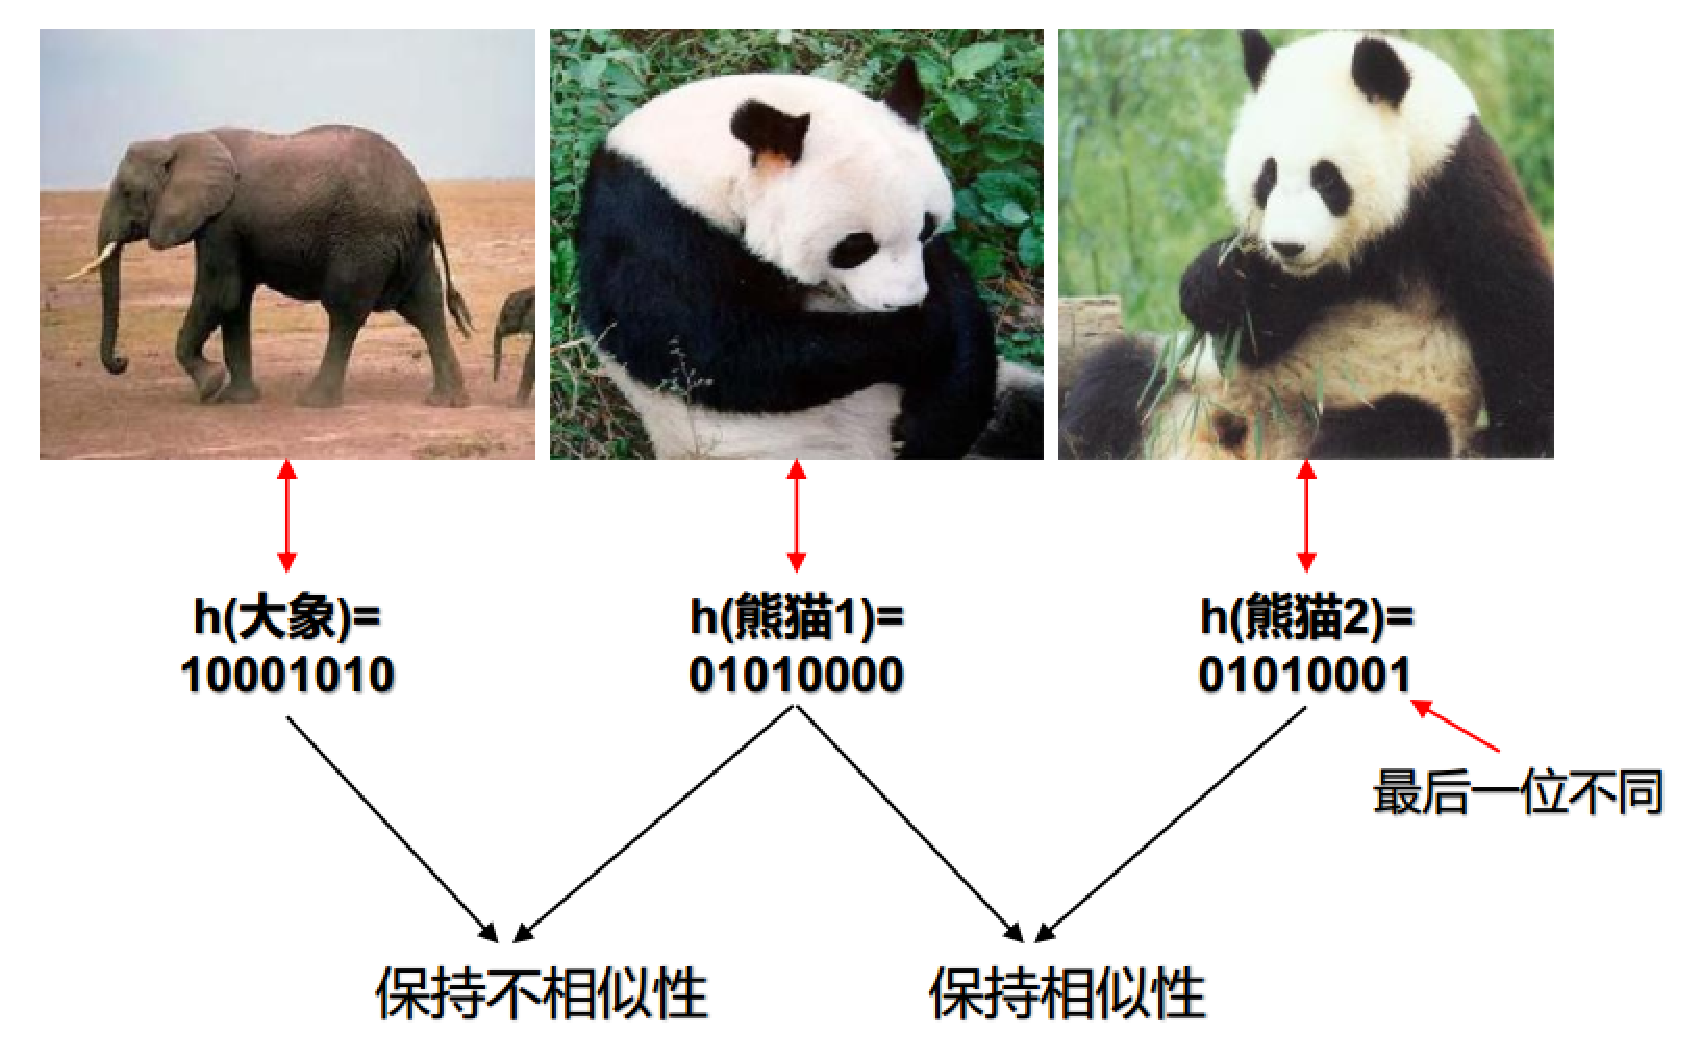
\includegraphics[width=0.8\textwidth]{figures/hash_example.eps}
\caption{��ϣ����ʾ��}
\label{hash_example}
\end{figure}

\subsection{�����}
\esubsection{Motivation of research}

��ϣ������ǰ�ܵ�ѧ����͹�ҵ��Ĺ㷺�������������ڹ�ϣ�����ܹ�����Ƚ������ݴ洢�ռ俪����������˵�����ʹ��\ 1024 �ֽڣ�1KB�����洢ÿ��ԭʼ������������������������һ��������������ݼ���ռ��\ 1GB �Ĵ洢�ռ䣬�������ÿ������������\ 64 λ��8B���Ĺ�ϣ������ʾ, ��洢�ռ�ֻ��Ҫ\ 8MB���ռ������½���\ 125 �����ڼ����ٶȷ��棬����ʹ�������������ϣ���ĺ������뼴�ɵõ���ͬ��ϣ��֮��������ԣ���˼����ٶȴ���������ɴ˿ɼ���ϣ������ʵ���ԣ�����֮�⣬��ϣ����ȡ�õļ����������ڲ����������𲽴ﵽʵ�õ�Ҫ�����ֳ������������Ч�ԡ�

��ǰ�Ѵ��ںܶ�����Ĺ�ϣ������Ȼ�������Ե�һģ̬�ļ��������������ͳ�ĵ�ģ̬��ϣ������ͬһģ̬���ݼ���м��������������ĺ���ͼ��ͼ�����Ӧ�á�������Ϣ�����Ŀ��ٷ�չ�����ݵı�ը�����������ݵı�����ʽҲ��������������´�ͳ�ĵ�ģ̬��ϣ�����޷����ģ̬�佻����������⣬��������ͼ����ͼ���ĵȣ����Ƕ�ģ̬��ϣ�����ǿ�ģ̬��ϣ\cite{bronstein10cmssh,masci14multimodal,zhen12probabilistic,Chen2017Predicting,ZhangPF17MM,luo2018sdmch,xu2016Dictionary} Ӧ�˶�������Ҫ˼��Ϊ�����ģ̬����ӳ�䵽һ�������ӿռ��У��ڹ����ӿռ��н���ͬģ̬��������Ϊ��ֵ��ϣ�벢���㲻ͬģ̬���ݼ�������ԡ�

Ŀǰ���кܶ��ģ̬��ϣ�����������ȡ���˲����Ŀ�ģ̬����Ч�����������м������������ܵ�������ڣ�һЩ��������ɢ���������ɳڻ����������ɵĹ�ϣ���нϴ��������ʹ�����չ�ϣ��ļ���Ч���½���Ҳ��һЩ����ֱ�ӽ�����ɢ�Ż�������������ѵ��ʱ��Ϊ���ۣ������Ż�����ʱ�������ӣ��ڼල��Ϣ��ѡ���ϣ��еķ���ѡ��ʹ��$\ n\times n$ �������Ծ�����������Ա��֣�����ᵼ����ѵ����ʱ�临�Ӷ�������$O(n^2)$����������������չ�����ģ���ݼ����Ѷȡ�

�ۺϿ�����������֮�󣬱������һ���µ��мල��ģ̬��ϣ�����������ھ���ֽ�Ŀ���չ��ɢ��ϣ���÷�����ԭʼ�����˻�����о���ֽ⣬����ϱ�ǩ��Ϣ������Ƕ��������һ�������ӿռ䣬�Ӷ������ܵı���ģ̬���ģ̬�ڵ����������ԣ�ͬʱ��ͨ��ʹ�ñ�ǩ������������Ծ��󣬸÷�����ѵ�����Ӷ�ʼ�������ݼ���ģ����Ϊ���Թ�ϵ���ɷ������չ�����ģ��ģ̬���ݼ��ϣ�Ϊ�˽����ɢ�Ż����⣬����������ת��������С��ѵ�������е���������ʹ�õ����Ż��ķ�ʽ����һ����С������

\section{�������о���״}
\esection{Related works}

���еĹ�ϣ�������¿ɸ����䴦��ģ̬������Ϊ���ࣺ��ģ̬��ϣ�Ϳ�ģ̬��ϣ����ͳ�ĵ�ģ̬��ϣ����ֻ����һ��ģ̬���ݣ�ͨ�������Ƚ��Ļ���ѧϰ���۹���Ŀ�꺯����ѧϰ��ϣ�����͹�ϣ�롣Ŀǰ���ֵ�ģ̬��ϣ�����ѱ���������ֳ����õĵ�ģ̬���ݼ������ܡ����ݹ�ϣ�������Ƿ��мල��Ϣ��ʹ�ã���ģ̬��ϣ�����ɷ�Ϊ�޼ල��ģ̬��ϣ����ල��ģ̬��ϣ���мල��ģ̬��ϣ��

ʵ��Ӧ���У����ڶ�ģ̬���ݵķ�����������ģ̬����֮��ļ�����Ϊؽ����������⣬��˿�ģ̬��ϣ����Ӧ�˶�������������ͼ����ͼ���ĵȡ���ģ̬��ϣ������һ���ؼ���������δ������Բ�ͬ���ʷֲ��Ķ�ģ̬���ݣ�Ϊ�˽��������⣬���еĿ�ģ̬��ϣ�������¿��Է�Ϊ���ࣺģ̬������ϣ�ͼ��ɹ�ϣ��ͬʱ�����ڽ��������ģ�ͱ��ֳ�ǿ���������ʾ��������ģ̬�Ϳ�ģ̬��ϣ����ʼ�����ѧϰ���ϣ���ȡ����׿Խ�ļ���Ч����

������ͨ�������������������չ������ϸ���ܵ�ǰѧ������ڹ�ϣ�������о���չ��

\subsection{�޼ල��ģ̬��ϣ����}
\esubsection{Unsupervised single-modal hashing methods}

�޼ල��ģ̬��ϣ�����������κμල��Ϣ�����ǩ��tag�ȣ���ֻ��ԭʼ����������ѧϰ��ϣ����������ԭʼ�ռ������ݵ�ľֲ��ṹ�����������ԡ����д������������׹�ϣ��Spectral Hashing, SH��\cite{weiss09sh}��ê��ͼ��ϣ��Anchor Graph Hashing, AGH��\cite{liu2011agh}���Խ̹�ϣ��Self-Taught Hashing, STH��\cite{zhang2010self}�� ����������ϣ��Iterative Quantization, ITQ��\cite{gong11itq}��ͼ��ɢ��ϣ��Discrete Graph Hashing, DGH��\cite{liu2014discrete}������չͼ��ϣ��Scalable Graph Hashing, SGH��\cite{jiang2015scalable}�ȡ�

�׹�ϣ��SH����ͼ�ָ�ĽǶȶ�ͼ����ж�ֵ���룬����ԭʼ��\ NP-hard ��ɢ�Ż���������ɳڣ�ͨ����ͼ������˹����������������ж�ֵ���������������յĹ�ϣ�����Ȼ���׹�ϣ�������\ $n \times n$ ��ͼ������˹����������ʱ�临�ӶȽϸߣ������ʵ��Ӧ�ù������Դ������⡣

Ϊ�˽���׹�ϣ���ͼ������˹���������ٶ�����ʱ�������⣬ê��ͼ��ϣ��AGH��ʹ�ý��ƽ���ͼ������ԭʼ��������˹ͼ�����������������ͨ������ê����ȷ��������ê��ͼ�ڽӾ���ĵ������ԣ��Ӷ�ʹ��ͼ������˹��������������������ʱ������ɣ�����ܹ��������������ϣ�롣

���ǵ���ͳ�Ĺ�ϣ����ֻ�Լ������������������ö���֮ǰδ������������Ӧ�Բ��õ����⣬�Խ̹�ϣ��STH��������ȶ���������ʹ�õ�ǰ���ܽϺõ��޼ල��ϣ��������$l$λ�Ĺ�ϣ�룬Ȼ��ʹ�����ɵĹ�ϣ����Ϊ�ල��Ϣ��ѵ��$l$����������Ϊ��ϣ�������Ӷ���߶�֮ǰδ�����IJ�ѯ��������Ӧ�ԡ�

���ǵ�����������ÿ�����ɷַ�����Principle Component Analysis, PCA�������ϵķ��ͬ��������˵���߷���\ PCA ����Я��������Ϣ����˴�ͳ��ϣ������ÿ��\ PCA ����������ͬ��Ŀ�Ĺ�ϣ��λ���ᵼ�¼������ܱ�����������ϣ��ITQ���ȶ�ԭʼ��������\ PCA ��ά�õ��м��ʾ��Ȼ�����������ת��������С���м��ʾ�͹�ϣ��֮����������Ӷ�ʹ�ø���\ PCA ����ķ������ƽ�⣬��ϣ�����ļ���Ч��Ҳ�����ߡ�

���ںܶ��޼ල��ϣ�������Ź�ϣ��λ�����Ӷ����������½���������Ҫ��ԭ��������Щ�������Ż����Բ������ɳ���ɢԼ���õ�ʵֵ��ʾ��ѵ��������Ը�ʵֵ��ʾ���ж�ֵ���õ����յĹ�ϣ�룬�����Ż�����������������������ͼ��ɢ��ϣ��DGH�������ɢ�Ż����������������ͬʱ����ê��ͼ����׽���ģ���ݼ��������Ľ��ڽṹ��

Ȼ����ͳ�Ļ���ͼ���޼ල��ϣ������Ȼ���ڹ���ͼ�ĸ߸��Ӷ����⣬�Ӷ����ܴﵽ���������Ч������˿���չͼ��ϣ��SGH������������ת������Ч�رƽ�����ͼ�ζ�������ʽ�������ƶ�ͼ���󣬲��ڴ˻����������һ��˳��ѧϰ��������λ��ʽѧϰ��ϣ������

\subsection{�мල��ģ̬��ϣ����}
\esubsection{Supervised single-modal hashing methods}

�мල��ģ̬��ϣ�������ø����ļල��Ϣ���������ݼ�������ԣ��Ӷ����õؽ��й�ϣѧϰ�������Ա��֣�ʹ��ԭʼ�ռ������ƣ������ƣ��������ں����ռ�����Ȼ���ƣ������ƣ����Ƚϵ��͵��мල��ģ̬��ϣ�����к˼ල��ϣ ��Kernel-based Supervised Hashing, KSH��\cite{liu12ksh}�� ����ල��ϣ��Latent Factor Hashing, LFH��\cite{zhang2014lfh}��������ϣ��Two-Step Hashing, TSH��\cite{lin2013tsh}�����ټල��ϣ��Fast Supervised Hashing, FastH��\cite{lin14fasthash}���ල��ɢ��ϣ��Supervised Discrete Hashing, SDH��\cite{shen15sdh}���в�����ɢ�ල��ϣ �� COlumn Sampling based DIscrete Supervised Hashing, COSDISH��\cite{kang16cosdish}��

��ǰ�Ĺ�ϣ����������̫�����ڴ��ģ��ͼ�����ݼ�����Ϊ���Ƕ���ֱ���Ż��������룬������Ϊ���������Ƿ�͹�ҷ�ƽ���ģ�������ʧ����̫���������������Ż�����˺˼ල��ϣ��KSH���Ƶ�����������͹�ϣ����ڻ��������ǵȼ۵ģ��������˼��������Բ��ɷֵ����ݽ����Ż����Ӷ���Ƴ��˻��������Ծ���ͺ˼�������ʧ��������ʹ����̰���㷨����λ����ϣ������

��������еĹ�ϣ����Ӧ�õ�һ��ʽ�Ĺ�ϣ���������Ż�����ͨ������ض���ʽ�����ϣ������ֽ�����������˷�����Ӧ���ݵ�����ԣ����ҿ��ܵ������Խ���ĸ����Ż����⡣������ϣ��TSH�������һ�������򵥵Ŀ�ܣ����ܹ���Ӧ��ͬ���͵���ʧ�����͹�ϣ�����������µ��ض������ϣ�����Ŀ���������ͨ������ʧ�������Ż����õ���ϣ�룬Ȼ���Թ�ϣ��Ϊ�ල��Ϣѵ������������ʽ�õ���ϣ������

���֮ǰ����ķ����Թ�ϣ������ͨ�����õ�ʵ�ַ����Ե��ֶζ�Ϊʹ�ú˹�ϣ��������\ KSH ��\ TSH��ʵ������˹�ϣ���������������������Թ�ϣ�����ļ������ܣ�Ȼ��������ά������ʱ���˺�����ѵ���Ͳ��Գɱ�Ҳ��֮���ӣ��Ӷ�����ʵ��Ӧ���е���Դ���㡣���������⣬���ټල��ϣʹ�þ�������Ϊ��ϣ�����ķ����Թ�ϣ�������Ӷ������˺˺��������ľ޴����ģ��Ҿ���������ѵ���Ͳ����ٶȿ��Ϊ��ҵ����ϲ������˸�����ʹ�ü�ֵ�����ټල��ϣ��FastH������������ϣ�IJ��ԣ���һ���Ƚ���ϣ����Ż�����ת��Ϊһ�������ƶ��ι滮��������λ����ϣ�룬�������˷ֿ�������ͼ�ָ�������õ���ϣ�룬�ڶ���ʹ�õ�һ���õ��Ĺ�ϣ����Ϊ�ල��Ϣ�����\ Adaboost ���ɲ�����ѵ����������Ϊ��ϣ������

����ල��ϣ��LFH������DZ������ģ�ͽ��ɶ�����֮�������Ե���Ȼ�������ŵؽ�ģΪ��Ӧ���ݵ�֮��ĺ�������ĺ�����ͬʱΪ�˶Դ��ģ������н�ģ�������һ�����ѧϰ�Ż�������ʱ��������ڿ���ѧϰ�������Դﵽ�������ܺ�Ч�ʵĴ��������

�ල��ɢ��ϣ��SDH��û�в��ö���ɢԼ�������ɳڵ�������Ҳ���ǹ�ϣ����ѵ��������һֱ����ɢ�Ķ�ֵ��������Ϊ��ͳ�Ļ����ɳڼ����Ĺ�ϣ�����ᵼ�½ϴ�����������DZ�����ɢԼ���������Ż��Ѷȣ����\ SDH ������ɢѭ�������½���Discrete Cyclic Coordinate descent, DCC����������λ��ϣ�������⣬ͨ����������ѵ���������õ����õĹ�ϣ�롣

Ϊ�˽��֮ǰ��ϣ������ʱ�ͶԴ��ģ���ݼ���չ�Բ�����⣬�в�����ɢ�ල��ϣ��COSDISH�����õ����Ż��ķ�ʽ����ÿ�ε����У����������ƶȾ����жԼ��н��в�����Ȼ�󽫹�ϣ��ֽ�Ϊ�����֣��������ֿ�������ɢ��ʽ�����Ż���

\subsection{��ȵ�ģ̬��ϣ����}
\esubsection{Deep single-modal hashing methods}

����������ģ��չ�ֳ�����ǿ���������ʾ������һЩ�������ģ�͵ĵ�ģ̬��ϣ����Ҳ�������������������ϣ��Convolutional Neural Network Hashing, CNNH��\cite{xia14cnnh}����������ѧϰ����ȼල��ϣ��Deep Pairwise-Supervised Hashing, DPSH��\cite{li2015dpsh}�������������ϣ��CNNH���Ѿ���������ֱ�����ϣ�㷨�����˽�ϣ������������ϣ��˼�룬����ͨ��ʹ�����ƶȾ�����Ϊ�ල��Ϣ�õ���ϣ�����Ȼ�󽫾��������磨CNN����Ϊ��ϣ������Ͻ�������ʧ�����Թ�ϣ����Ϊ�ල��Ϣ���Ӷ�����ϣ����ѧϰ����ת��Ϊ���ǩ�������⣬����������\ softmax ��ʧ��������һ���������ܡ�ʵ�����\ CNNH ��ȴ�ͳ��dz���ϣ����ȡ��������������������Ȼ��������ϣ��͹�ϣ������ѧϰ���̷�Ϊ������������Ĺ��̣���Ȼ���Ƕ˵��˵ķ�����������ѧϰǿ���������ʾ������û�б�����ھ򡣻�������ѧϰ����ȼල��ϣ��DPSH���������һ���˵��˵Ŀ�ܣ�ͬʱ���й�ϣ���������������磩�Լ���ϣ���ѧϰ���Ӷ�ʹ��ͼ��������ȵõ���һ��������

\subsection{ģ̬������ģ̬��ϣ����}
\esubsection{Modality-specific cross-modal hashing methods}

ģ̬������ģ̬��ϣ������ÿ��ģ̬ѧϰһ�����������ռ��еĹ�ϣ�룬���ģ̬���������й�ϣ��Cross-Modal Similarity Sensitive Hashing, CMSSH��\cite{bronstein10cmssh}�����ӽǹ�ϣ��Cross-View Hashing, CVH��\cite{kumar11cvh}�������򻯹�ϣ��Co-Regularized Hashing, CRH��\cite{zhen2012crh}����ý���ϣ��Inter-Media Hashing, IMH��\cite{song13imh}�ȡ�

��ģ̬���������й�ϣ��CMSSH�������������еĹ�ϣ������չ�����ģ��ģ̬�����ϣ����Խ���ͬ��ģ̬Ƕ�뵽���������ռ��У�����ÿ��ģ̬����ͶӰ����ϣ�뽨ģΪ��ֵ�������⣬��ʹ�ñ�׼\ AdaBoost ����ѧϰ��

���ӽǹ�ϣ��CVH�����׹�ϣ��SH���Ķ�ģ̬��չ�����Ƚ�ѧϰ��ϣ�������������Ϊ���ģ��ģ̬�����ϵ��ɳ�Լ����С�����⣬Ȼ��ͨ������������ֵ�����������С�����⡣

�����򻯹�ϣ��CRH��ͨ�����\ DC��Difference of Convex functions, ͹����֮��IJ��죩������ѧϰÿ��λ�Ĺ�ϣ������ͬʱͨ��\ boosting ���̽��ж�λ��ѧϰ���Ա����˳�����С���ɹ�ϣ���������ƫ�

��ý���ϣ��IMH��̽�������Բ�ͬ����Դ�Ķ���ģ̬����֮�������ԣ�������ģ̬��һ���Ժ�ģ̬�ڲ�һ���ԣ��Է���һ����ͬ�ĺ����ռ䣬��ʹ�����Իع������ģ����ѧϰ����ض�ģ̬�Ĺ�ϣ������

\subsection{���ɿ�ģ̬��ϣ����}
\esubsection{Integrated cross-modal hashing methods}

Ȼ��ģ̬������ϣ��ҪΪÿһ��ģ̬�����������ݿ���Ӧ�Ĺ�ϣ�룬��������˼����ʹ洢�Ĵ��ۡ���Զ��ԣ����ɹ�ϣ����Ϊ����ģ̬Ѱ��һ�����������ռ䣬����ģ̬�����ݾ�ӳ�䵽���������ռ������ɶ�Ӧ��ϣ�룬����ֻ��Ҫһ�����������ݿ��ϣ�룬�Ӷ�������ģ̬������ϣ�޴�ļ����ʹ洢���ۣ����Ӧ�ø�Ϊ�㷺����������ϡ���ϣ��Latent Semantic Sparse Hashing, LSSH��\cite{zhouJ14LSSH}��Эͬ����ֽ��ϣ��Collective Matrix Factorization Hashing, CMFH��\cite{ding14cmfh}�������������󻯹�ϣ��Semantic Correlation Maximization, SCM��\cite{zhang14scm}�����屣�ֹ�ϣ��Semantics Preserving Hashing, SePH��\cite{lin15seph}���мල����ֽ��ϣ��Supervised Matrix Factorization Hashing, SMFH��\cite{Liu16smfh}����ɢ��ģ̬��ϣ��Discrete Cross-modal Hashing, DCH��\cite{xu17dch}�ȡ�

��ǰ�������ģ̬��ϣ����ͨ������ͶӰ���칹����Ƕ�뵽���ϳ���ռ��У�Ȼ����Щ����δ�ܸ���Ч���ֺ�����蹵������߼�DZ��������Ϣ�����������ϡ���ϣ��LSSH��ʹ��ϡ����벶��ͼ��������ṹ�Լ�ʹ�þ���ֽ������ı���ѧϰDZ�ڵ�������Ȼ������ģ̬ѧϰ����DZ��������Ϣӳ�䵽����������ռ��У��Ӷ����õ��ֺ�����蹵��

Эͬ����ֽ��ϣ��CMFH������һ������������ÿ��ģ̬������ͬ�Ĺ�ϣ�룬���������Բ�ͬģ̬��ijЩ��ϣ�����ϻ�����ͨ���Բ�ͬģ̬����ʹ�ô�DZ�����ӵ�Эͬ����ֽ�ģ����ѧϰͳһ�Ĺ�ϣ�롣

�����������󻯹�ϣ��SCM��ͨ�������������Խ������ǩ���ɵ�ѧϰ�����У�ͨ��������ʽ����ɶ������Ծ���Ӷ������������мල��Ϣ��������ʱ�临�Ӷȵ�ѵ������ʹ�����չ�����ģ���ݼ��������һ��˳��ѧϰ��������λѧϰ��ϣ������ÿ��λ�Ĺ�ϣ�����б�ʽ�⣬���ѵ�������в���Ҫ��������ֹͣ������

���屣�ֹ�ϣ��SePH����һ�֡������ߡ��ķ����Կ�ģ̬��ϣ��������������ϣ��TSH���Ķ�ģ̬��ϣ��չ������ѵ�����ݼ��������������Ϊ�ල��Ϣ��SePH ���������Ծ���ת��Ϊ���ʷֲ�����ʽ���Ӷ��Ը��ʷֲ�������ѵ�����ݵ����������ԣ�Ȼ��ʹ�ú˻����߼��ع飨Logistic Regression����ʵ�ַ����ԵĹ�ϣ��������ͨ��\ Kullback-Leibler ɢ����С���������뺣���ռ��еĴ�ѧϰ��ϣ����ơ�
%���屣�ֹ�ϣ��SePH�������������Ծ�����Ϊ�ල��Ϣ��Ȼ������ת��Ϊ���ʷֲ�������ͨ����С��Kullback-Leibler ɢ�ȡ�

�мල����ֽ��ϣ��SMFH��ͨ����ͬģ̬�ķǸ�Эͬ����ֽ��������ģ̬��ϣ���⣬ͨ��ͼ���������ֶ�ģ̬ԭʼ����֮��������ԣ�ͬʱ�������ǩ����ʱ���ϲ���ѧϰ�����У��Ӷ���߼�����׼ȷ�ԡ�

��ɢ��ģ̬��ϣ��DCH���Ǽල��ɢ��ϣ��SDH���ڶ�ģ̬�����µ���չ��ͬ����ѵ�������б��ֹ�ϣ�����ɢ���Բ�������ɢѭ�������½���DCC����������λ��ϣ�������⣬���������˲���ѵ�����ۣ������յĹ�ϣ�������ܵõ��˴����������

\subsection{��ȿ�ģ̬��ϣ����}
\esubsection{Deep cross-modal hashing methods}

����֮�⣬����������ģ�͵Ŀ�ģ̬��ϣ����Ҳ�ѱ����������ȡ����ͻ���Խ�չ������ȿ�ģ̬��ϣ��Deep Cross-Modal Hashing, DCMH��\cite{jiang2017dcmh}������Ӿ������ϣ��Deep Visual-Semantic Hashing, DVSH��\cite{cao2016dvsh}���Կ���ģ̬������Adversarial Cross-Modal Retrieval, ACMR��\cite{wang2017acmr}�ȡ�

��ȿ�ģ̬��ϣ��DCMH��\cite{jiang2017dcmh}��һ���˵��˵Ŀ�ģ̬��ϣѧϰ��ܣ�������ѧϰ�͹�ϣ��ѧϰ���ɵ�ͬһ�����ѧϰ����У�Ϊÿ��ģ̬�ṩһ����������磬������ѧϰ������ʼ�ձ��ֹ�ϣ�����ɢ���ԡ�

����Ŀǰ�������ģ̬��ϣ���������ܲ�׽ͼ��Ŀռ������Ժ��ı����ӵ�ʱ�䶯̬��ѧϰǿ���������ʾ�ͼ��ٲ�ͬģ̬�������ԵĿ�ģ̬Ƕ�룬�������Ӿ������ϣ��DVSH��\cite{cao2016dvsh}����ͼ��ľ��������磨Convolutional Neural Network, CNN�����ı���ѭ�������磨Recurrent Neural Network, RNN���Լ�������������Ľṹ������ԵĿ�꺯������ʵ�������Ա��ֺ͸�������ϣ���ѧϰ��

Ȼ�������еĻ������������Ŀ�ģ̬��������������ע�ڱ���������ϵĿ�ģ̬���һ��ͼƬ��һ���ı���֮��ijɶ������ԣ�����ʵ�ж���һ��ģ̬��һ��������˵������ͬһ��ģ̬�д��ڶ�����岻ͬ����������˽�ͨ�����ֳɶ������Եķ�ʽѧ���Ĺ�����ʾ�ռ����޷���ֱ������ݵ�������ģ̬����ṹ�ġ��Կ���ģ̬������ACMR��\cite{wang2017acmr}�����˶Կ��������磨Generative Adversarial Networks, GAN����˼�룬ͨ������ӳ������ģ̬������������ɲ��ֵ������С��������������ŵĹ��������ӿռ䣬����ȷ��ѧϰ���Ĺ��������ʾͬʱ����ͬһģ̬�еĿ��������Լ�ģ̬֮��ͬһ�����IJ����ԣ��Ӷ�ʹ��ģ̬���ģ̬�ڵ�����ṹ�ܹ��õ����õı��֡�

\section{������Ҫ����}
\esection{Main contents}

Ŀǰ�Ѿ�������������Ŀ�ģ̬��ϣ������Ȼ����Ȼ����һЩؽ���Ż������⣺1������������ɳ��˹�ϣ�����ɢԼ���Ա����Ż���Ȼ��ѧϰ��ʵֵ������Ϊ�����ƹ�ϣ�룬����ܲ����ܴ��������ʹ��õĹ�ϣ�벻�ɿ���2��һЩ������������ɢ��ģ̬��ϣ��DCH��\cite{xu17dch}����ͼ������ɢѭ�������½���DCC��������������ɢԼ������λ����Ż����⣬Ȼ����λ�Ż�ʹ��ѵ���dz���ʱ��3������һЩ����������\ $n\times n$ �������Ծ�������������֮��������ԣ�����\ SePH ��\ FSH�������ڴ��ģ���ݼ���˵���⽫���Ӽ��㸴���Ժ��ڴ�ɱ���������Щ����������չ�����ӽ���չ������ͨ�õķ��������ѡȡ���ݼ����Ӽ�����ѵ�������������������������ֵ��¿�ģ̬�����ļ������������½���

Ϊ�˽��������ս�����������һ����ӱ�ļල��ģ̬��ϣ�����������ھ���ֽ�Ŀ���չ��ɢ��ϣ��SCRATCH�������ڲ�ͬģ̬������ͬ��DZ������ռ䣬�����DZ�ڵ�����ռ�����ʵ�ı�ǩ����ռ���һ�µļ��裬SCRATCH �����ڷ����Ժ˻��������������Эͬ����ֽ⣨CMF����ϱ�ǩ������Ƕ�����ҵ�DZ�ڵ�����ռ䣬�Ӷ�����ģ̬���ģ̬�ڵ������ԣ�Ȼ��ͨ��������ת��������С��ѵ����������������ͬʱ��ѧϰ������Ҫ�Ĺ�ϣ��͹�ϣ����������ѵ��������ֻ�õ��������ǩ���dzɶԵ������Ծ���SCRATCH ��������ʱ����ѵ����ϣ�����ѵ�������б����˹�ϣ�����ɢԼ����ʹ��ѧϰ���Ĺ�ϣ���������ߡ�


\section{������֯�ṹ}
\esection{Thesis framework}

�����ĵ���֯�ṹ���£�

��һ�½����˱��Ŀ�����о����������壬�����˹������о���״������ڵ����⣬�Ӷ��������ĵ���Ҫ���������µ㣻

�ڶ�����ϸ�����˱�������Ŀ�ģ̬��ϣ����������������ʧ������ơ��Ż����̡��㷨��չ�Լ����ӶȺͶ���������

�����½�����ȫ�����꾡��ʵ�飬�����㷨��ʵ��ϸ�ڡ��Աȷ����Լ�ʵ�����ķ�����

���һ�¶�ȫ�ĵ���Ҫ���µ㼰����֮���������ܽᣬ��������ĵIJ�������˶�δ��������չ����


\chapter{\quad\quad ���ھ���ֽ�Ŀ���չ��ɢ��ϣ}
\echapter{Scalable Discrete Matrix Factorization Hashing}
\label{chap2}


���½��������\ SCRATCH �ĸ��������Ŷ��塢��ʧ������ơ��Ż����̡��㷨��չ�Լ�ʱ�临�ӶȺ���ض���������ϵͳ�IJ�����\ SCRATCH �����ۻ�����������Ҫ��Ϊ���С�ڣ��ֱ�Ϊ��������SCRATCH �㷨���Ż����̡��㷨�����Լ�����С�ᡣ

\section{����}
\esection{Introduction}

���������ݵĹ�ģ������ɱ�ը��������������ݵĴ洢������Ч������˾޴����ս������ϣѧϰ�ṩ��һ�ִ洢С������Ľ������������ܵ��˹㷺��ע����ϣѧϰ��Ŀ����ͨ��ԭʼ����ӳ��ͺ����ռ�������Ա������õ���Ӧ�Ĺ�ϣ����м�����ͬʱ�������Ĺ�ϣ��Ӧ�������ĸ����ԣ�1) �����Ա��֣�ԭʼ�ռ������ƣ������ƣ��������ں����ռ���ҲӦ���ƣ������ƣ���2) �����ԣ���ϣ�����λ֮��Ӧ�û������������Ӧ�������Ի�����Թ�ϵ��3) ƽ���ԣ���ϣ���ÿ��λ����\ $50\%$ �Ŀ�����ȡ\ 1 ����\ $-1$��4) ��ɢ�ԣ������Թ�ϣ���λֻ��ȡ\ 1 ��\ $-1$ ����ֵ������ģ̬��ϣ�Թ�ϣ�������Ҫ��������ߣ���Ҫ��֤����ģ̬���ģ̬�ڵ������Ա���Ҫͬʱ��ѵ�����������㣬��ͨ��Ҫ�����ģ̬����ӳ�䵽һ�������ӿռ��С�

Ϊ�˵õ������������Եĸ�������ϣ����������ݼ������ܣ����������һ��ȫ�µĻ��ھ���ֽ�Ŀ���չ��ɢ��ϣ������SCRATCH�����÷�����ͬʱѧϰ��ϣ�����͹�ϣ�룬��ʹ��Эͬ����ֽ⣨CMF���ͱ�ǩ����Ƕ����ʵ�ֱ���ģ̬���ģ̬�ڵ������ԣ��������������ת����������ѵ�������й�ϣ�����ɢ���ԡ�������Ҫ���׿��ܽ�Ϊ���¼��㣺
\begin{itemize}
%\vspace{-3mm}
\item ���һ��ȫ�µ��мල��ģ̬��ϣ�������Ӷ��ܹ���Ч�ز�׽��̬���������֮���������ϵ��ͨ������Эͬ����ֽ⣨CMF���ͱ�ǩ����Ƕ�룬�÷����ɳ���������еļල������Ϣ��
%\vspace{-3mm}
\item ���һ�ֵ����Ż��IJ��������\ SCRATCH �е��Ż����⣬ͬʱʹ���Ż���ʱ�临�Ӷ���������ݼ��Ĺ�ģ�����Թ�ϵ���Ӷ��������׵ؽ�����չ�����ģ���ݼ��ϡ�����֮�⣬���ڵ����Ż�ģʽ��SCRATCH ������ѵ�������б��ֹ�ϣ�����ɢ���ԣ��Ӷ���������������
\item �������������õĻ�׼���ݼ�������ֵ�ǰ�Ƚ���dz�����ȵĿ�ģ̬��ϣ���������˶Ա�ʵ�飬�����ʾ\ SCRATCH �ڿ�ģ̬���������Ͼ����������з�������ѵ���ٶȴ��������
\end{itemize}

\section{SCRATCH�㷨}
\esection{SCRATCH method}

\subsection{���Ŷ���}
\esubsection{Notations}

����\ $\bm{\mathcal{O}}=\{\textbf{o}_1,\textbf{o}_2,...,\textbf{o}_n\}$ ����\ $n$ ��������ѵ�������ϣ����� $\textbf{o}_i=\{\textbf{x}^{(1)}_i,...,\textbf{x}^{(m)}_i\}$ �ǵ�\ $i$ ��������\ $m$ ����ģ̬��������ʧһ���ԣ���һ������ÿ��ģ̬���������������Ļ��ģ���\ $\sum_{i=1}^{n}\textbf{x}^{(j)}_i=\textbf{0}, j=1,...,m$������\ $\textbf{L} \in \mathbb{R}^{l \times n}$ ��Ϊ��ʵ�ı�ǩ��������\ $l$ ������������������\ $\textbf{x}_i$ ���ڵ�\ $k$ �࣬��\ $\textbf{L}_{ki}=1$������Ϊ\ 0��$\textbf{B}\in \{-1,1\}^{r \times n}$ �Ǵ�ѧϰ�Ĺ�ϣ�����$\left \lVert \bm{\cdot} \right \rVert _F$ ���������\ Frobenius ������$sgn(\bm{\cdot})$ �����������\ $sign$ �������������£�
\begin{equation}
\label{sign}
    \begin{split}
    sgn(x) = \left\{
    \begin{aligned}
    1\  &&x>0 & ;\\
    -1\  &&x\leq0 & .
    \end{aligned}
    \right.
    \end{split}
\end{equation}

\subsection{Эͬ����ֽ�}
\esubsection{Collective matrix factorization}

Эͬ����ֽ⣨CMF��������Ŀ����������һ�ֵ���������ʾ����ͨ������ԭʼ���ݾ������Ƴ�������Ϣ��������˵��ͨ��������Ϊ\ $r$ �ľ���\ $\textbf{U} \in \mathbb{R}^{d \times r}$ ��\ $\textbf{V} \in \mathbb{R}^{r \times n}$ ��������������ݾ���\ $\textbf{X} \in \mathbb{R}^{d \times n}$������\ $n$ ������������������$d$ ������ά�ȣ�$r$ ���������ӵ�������

ֱ���ϣ�һ����ģ̬�����IJ�ͬģ̬�����Ķ���ͬһ��ʾ�������ʾ����ģ̬������ͬ��������Ϣ������������ȼ��費ͬģ̬������һ����Эͬ����ֽ⣨CMF���ھ������������ռ䣬�ɴ˿ɶ�ÿ��ģ̬�����¹�ʽ��ʾ��
\begin{equation}
\label{mf_info}
    \min_{\textbf{U}_t,\textbf{V}} \lambda_t\parallel \textbf{X}^{(t)}-\textbf{U}_t\textbf{V} \parallel^2_F+\gamma (\parallel \textbf{U}_t \parallel^2_F+ \parallel \textbf{V} \parallel^2_F),
\end{equation}
 ����\ $\textbf{X}^{(t)} \in \mathbb{R}^{d_t \times n}$ ��ѵ�����ĵ�\ $t$ ��ģ̬���ݣ�$\textbf{U}_t \in \mathbb{R}^{d_t \times r}$��$\textbf{V} \in \mathbb{R}^{r \times n}$��$d_t$ �ǵ�\ $t$ ��ģ̬������ά�ȣ�$r$ ����������������$\lambda_t$ ��\ $\gamma$ ��ƽ�������$\Sigma_{t=1}^m \lambda_t = 1$���Ҿ���\ $\textbf{V}$ ��ÿ��������\ $\textbf{v}_i$ ����������ռ��һ����������������ͨ����ȡ���Ĵ�����\ $r$ ����������������һ������������

\subsection{���������Ա���}
\esubsection{Preserving label consistency}

ͬһ�����IJ�ͬģ̬��ԭʼ�ռ��й�����ͬ�������ǩ����˸�������Эͬ����ֽ⣨CMF���ھ���Ĺ�����������ռ��е�������ʾӦ����ԭʼ�ռ����ͬ���������ǩ��������ù���������ʾ�ɱ��ع鵽��Ӧ������ǩ�ϡ�ͨ�����ַ�ʽ����ʽ�������ǩ��Ϣ�ɱ�Ƕ�뵽ѧ���Ĺ��������ռ��У��Դ�����֤ѧ�������������ʾ�����˺ͱ�ǩ��ͬ������һ���ԡ�Ϊ��ʵ���������屣�ֹ����������˹�ʽ \ \eqref{labelinfo} ���£�
\begin{equation}
\label{labelinfo}
    \min_{\textbf{G},\textbf{V}} \alpha \parallel \textbf{L}-\textbf{G}\textbf{V} \parallel^2_F+\gamma \parallel \textbf{G} \parallel^2_F,
\end{equation}
 ����\ $\textbf{L}$ ����ʵ��ǩ����$\textbf{G} \in \mathbb{R}^{l \times r}$ ��ӳ�����, $l$ �����������$\alpha$ ��һ��ƽ�������


\subsection{ӳ�亯��ѧϰ}
\esubsection{Learning mapping functions}

Ϊ��ʵ�ֿ�ģ̬���������ȼ���һ�������ĸ���ģ̬���ݶ����Ա�ӳ�䵽��ͬ�����������ӿռ��У����\ SCRATCH ��ÿ��ģ̬ѧϰһ�������Ĺ�ϣ�������Ӷ�������ÿ��ģ̬��ԭʼ����ͨ�����ԵĹ�ϣ����ӳ�䵽�����Ĺ����ӿռ��С������������輰Ŀ��ɵõ���ʽ \ \eqref{mapping}��
\begin{equation}
\label{mapping}
    \min_{\textbf{P}_t,\textbf{V}} \mu \parallel \textbf{V}-\textbf{F}_t(\textbf{X}^{(t)}) \parallel^2_F + \gamma \parallel \textbf{P}_t \parallel^2_F,
\end{equation}
����\ $\textbf{F}_t(\textbf{X}^{(t)})=\textbf{P}_t\textbf{X}^{(t)}$ �ǵ� $t$��ģ̬�Ĺ�ϣ������$\mu$ ����Ӧ��ƽ�������


\subsection{��ϣ��ѧϰ}
\esubsection{Learning hash codes}

��ͨ��Эͬ����ֽ⡢���������Ա����Լ���ģ̬ӳ�亯���Ľ��ѵ���õ�����������ʾ����\ $\textbf{V}$ ֮����һ���ѵ�������ν�����������ʾ����\ $\textbf{V}$ ��ʾΪ��Ӧ�Ĺ�ϣ�����\ $\textbf{B}$��ͬʱ��Ҫ��ӳ������б��ֹ�ϣ�����ɢ���ԡ���ͳ�Ĺ�ϣ�������ȿ��ǵĴ��Ϊ�ȶԹ�ϣ�����ɢ���Խ����ɳڣ����Եõ���ʵֵ��ʾ���ж�ֵ�����ڱ����м��ѵõ���\ $\textbf{V}$ ʹ��\ $sign$ �������ж�ֵ�����������Ĺ�ϣ�����\ $\textbf{B}$����\ $\textbf{B} = sgn(\textbf{V})$��

Ȼ�������ɳڵĹ�ϣ����������ѵ��������δ�ܱ�����ɢ���ԣ�����ѡ��ѵ��������ʵֵ����\ $\textbf{V}$ ��ֵ������ᵼ�µ�����������ʾ����\ $\textbf{V}$ ijһά�ϵ�ʵֵ�ķֲ��������������Χʱ��ԭʼ�ռ������Ƶ������ڸ�ά�����ɵĹ�ϣ�벢��һ�£�ʹ���ɳ�ʹ�õļ򵥵�������ʽ���п��ܻ���������Ա��ֹ��̳���ƫ�����ɳڷ���ͨ������ɺܴ�����������ǵ�������⣬SCRATCH ��\ ITQ\cite{gong11itq} �л����У����������������ת�������Ѿ�����ɢ���ԵĹ�ϣ�������뵽ѵ���У��Ӷ��ﵽ��С����������Ŀ�ģ���˶��幫ʽ\ \eqref{hash} �������������ת����͹�ϣ�������Ϊһ�����Ż��������Эͬѵ����
\begin{equation}
\label{hash}
    \begin{split}
        &\min_{\textbf{B},\textbf{R}} \parallel \textbf{B}-\textbf{R}\textbf{V} \parallel^2_F,\\
        &s.t. \ \ \ \textbf{B} \in \{-1,1\}^{r \times n}, \textbf{R}\textbf{R}^\top=\textbf{I},
    \end{split}
\end{equation}
����\ $\textbf{R} \in \mathbb{R}^{r \times r}$ ��Ϊ���������ת����$\textbf{B}$ ������ѵ�������Ĺ�ϣ�����$r$ Ϊ��ϣ�볤�ȡ�ֵ��һ����ǣ���С�ڣ�2.3�����Ż�������ʾ��ͨ���������������ת����\ $\textbf{R}$��SCRATCH ��ѵ�������б�������ɢ���ԣ���˿��Լ���̶��ϱ���֮ǰ�����ɳڼ����Ĺ�ϣ�����������ľ޴��������

\subsection{�����˻�}
\esubsection{Feature kernelization}

Ϊ�˲�׽��ͬģ̬�ķ����Խṹ�����ǽ�һ�����Ż������в����˺˻��������������ԭʼ���������ѹ�ʽ\ \eqref{mf_info} ��\ \eqref{mapping} �е�ԭʼ��������$X$ʹ�ú˻������\ $\bm{\phi}(\textbf{X})$ ���棬������˵������ʽ\ \eqref{mf_info} ����Ϊ��ʽ\ \eqref{kernel-2}����ʽ\ \eqref{mapping} ����Ϊ\ \eqref{mapping-2}��
\begin{equation}
\label{kernel-2}
    \min_{\textbf{U}_t,\textbf{V}} \lambda_t\parallel \bm{\phi}(\textbf{X}^{(t)})-\textbf{U}_t\textbf{V} \parallel^2_F+\gamma (\parallel \textbf{U}_t \parallel^2_F+ \parallel \textbf{V} \parallel^2_F),
\end{equation}
\vspace{-10mm}
\begin{equation}
\label{mapping-2}
    \min_{\textbf{P}_t,\textbf{V}} \mu \parallel \textbf{V}-\textbf{F}_t(\bm{\phi}(\textbf{X}^{(t)})) \parallel^2_F + \gamma \parallel \textbf{P}_t \parallel^2_F,
\end{equation}
����\ $\bm{\phi}(\textbf{x})$ ������\ $\textbf{x}$ �ķ�����Ƕ���������

����ʹ��֮ǰ��\ SDH\cite{shen15sdh}��DCH\cite{xu17dch} ���õ�\ RBF �˺�����ʵ�ַ�����ӳ�䣬��\ $\bm{\phi}_i(\textbf{x})=exp(\frac{-\parallel \textbf{x} - \textbf{a}_i \parallel_2^{2}}{2\sigma^{2}})$������\ $\{\textbf{a}_j\}_{j=1}^q$ �Ǵ�ѵ�����������ѡȡ��\ $q$ ��ê�㣬���Ľ����趨Ϊ\ $q=500$��$\sigma$ �Ǻ˿��ȣ��ɹ�ʽ\ \eqref{kernel_width} �����㣺
\begin{equation}
\label{kernel_width}
    \sigma=\frac {1}{nq}\sum_{i=1}^n\sum_{j=1}^q\parallel\textbf{x}_i-\textbf{a}_j\parallel_2
\end{equation}


\subsection{ȫ��Ŀ�꺯��}
\esubsection{Overall objective function}

����ʽ\ \eqref{labelinfo}��\ \eqref{hash}��\ \eqref{kernel-2}��\ \eqref{mapping-2} ���ϵ�һ��󣬿ɵõ�ȫ��Ŀ�꺯�����繫ʽ\ \eqref{obj} ��ʾ��
\begin{equation}
\label{obj}
    \begin{split}
        &\min_{\textbf{P}_t,\textbf{U}_t,\textbf{V}} \sum_{t=1}^m \lambda_t \parallel \bm{\phi}(\textbf{X}^{(t)})-\textbf{U}_t\textbf{V} \parallel^2_F\\
        &\ \ \ \ \ \ \ \ +\mu \sum_{t=1}^m \parallel \textbf{V}-\textbf{P}_t\bm{\phi}(\textbf{X}^{(t)}) \parallel^2_F+ \alpha \parallel \textbf{L}-\textbf{G}\textbf{V} \parallel^2_F\\
        &\ \ \ \ \ \ \ \ +\parallel \textbf{B}-\textbf{R}\textbf{V} \parallel^2_F + \gamma Re(\textbf{V}, \textbf{G}, \textbf{P}_t, \textbf{U}_t),\\
        &\ \ \ \ \ \ \ \ \ s.t. \ \ \ \sum_{t=1}^m \lambda_t=1, \textbf{B} \in \{-1,1\}^{r \times n}, \textbf{R}\textbf{R}^\top=\textbf{I},
    \end{split}
\end{equation}
����\ $m$ ����ģ̬������$\lambda_t$��$\mu$��$\alpha$ ��\ $\gamma$ ��Ϊƽ����������ڶ�Ŀ�꺯���еĸ�����ʧ�ṩȨ����ƽ������������Ŀ�����Ҫ�ԡ�Ȼ�����繫ʽ\ \eqref{obj} ��ʾ��SCRATCH ģ�ʹ�ѧϰ�IJ����ܶ࣬���ܲ����������߸�ģ�͵������������ȴͬʱ�����������ϵķ��գ�Ϊ������\ SCRATCH ģ�͵ķ������������ݰ¿�ķ�굶׼�����ޱ�Ҫ������ʵ�塱��ָ�������IJ��ü���������ķ�ʽ������ģ�Ͳ����ĸ��Ӷȣ�ͨ��ֱ���������Ż�Ŀ������ѡ��������պ�ģ�͸��Ӷ�ͬʱ��С��ģ�ͣ���ʽ\ \eqref{obj} �е�\ $Re(\textbf{V}, \textbf{G}, \textbf{P}_t, \textbf{U}_t)$ ��Ϊ���ڱ������ϵ����������Ϊ�������Ż�������������֮�͡�

Ϊ�˶Ա��ķ����и�ֱ�۵����⣬ͼ\ \ref{pipeline} չʾ��\ SCRATCH ��������:

\begin{figure}[htbp]
\centering
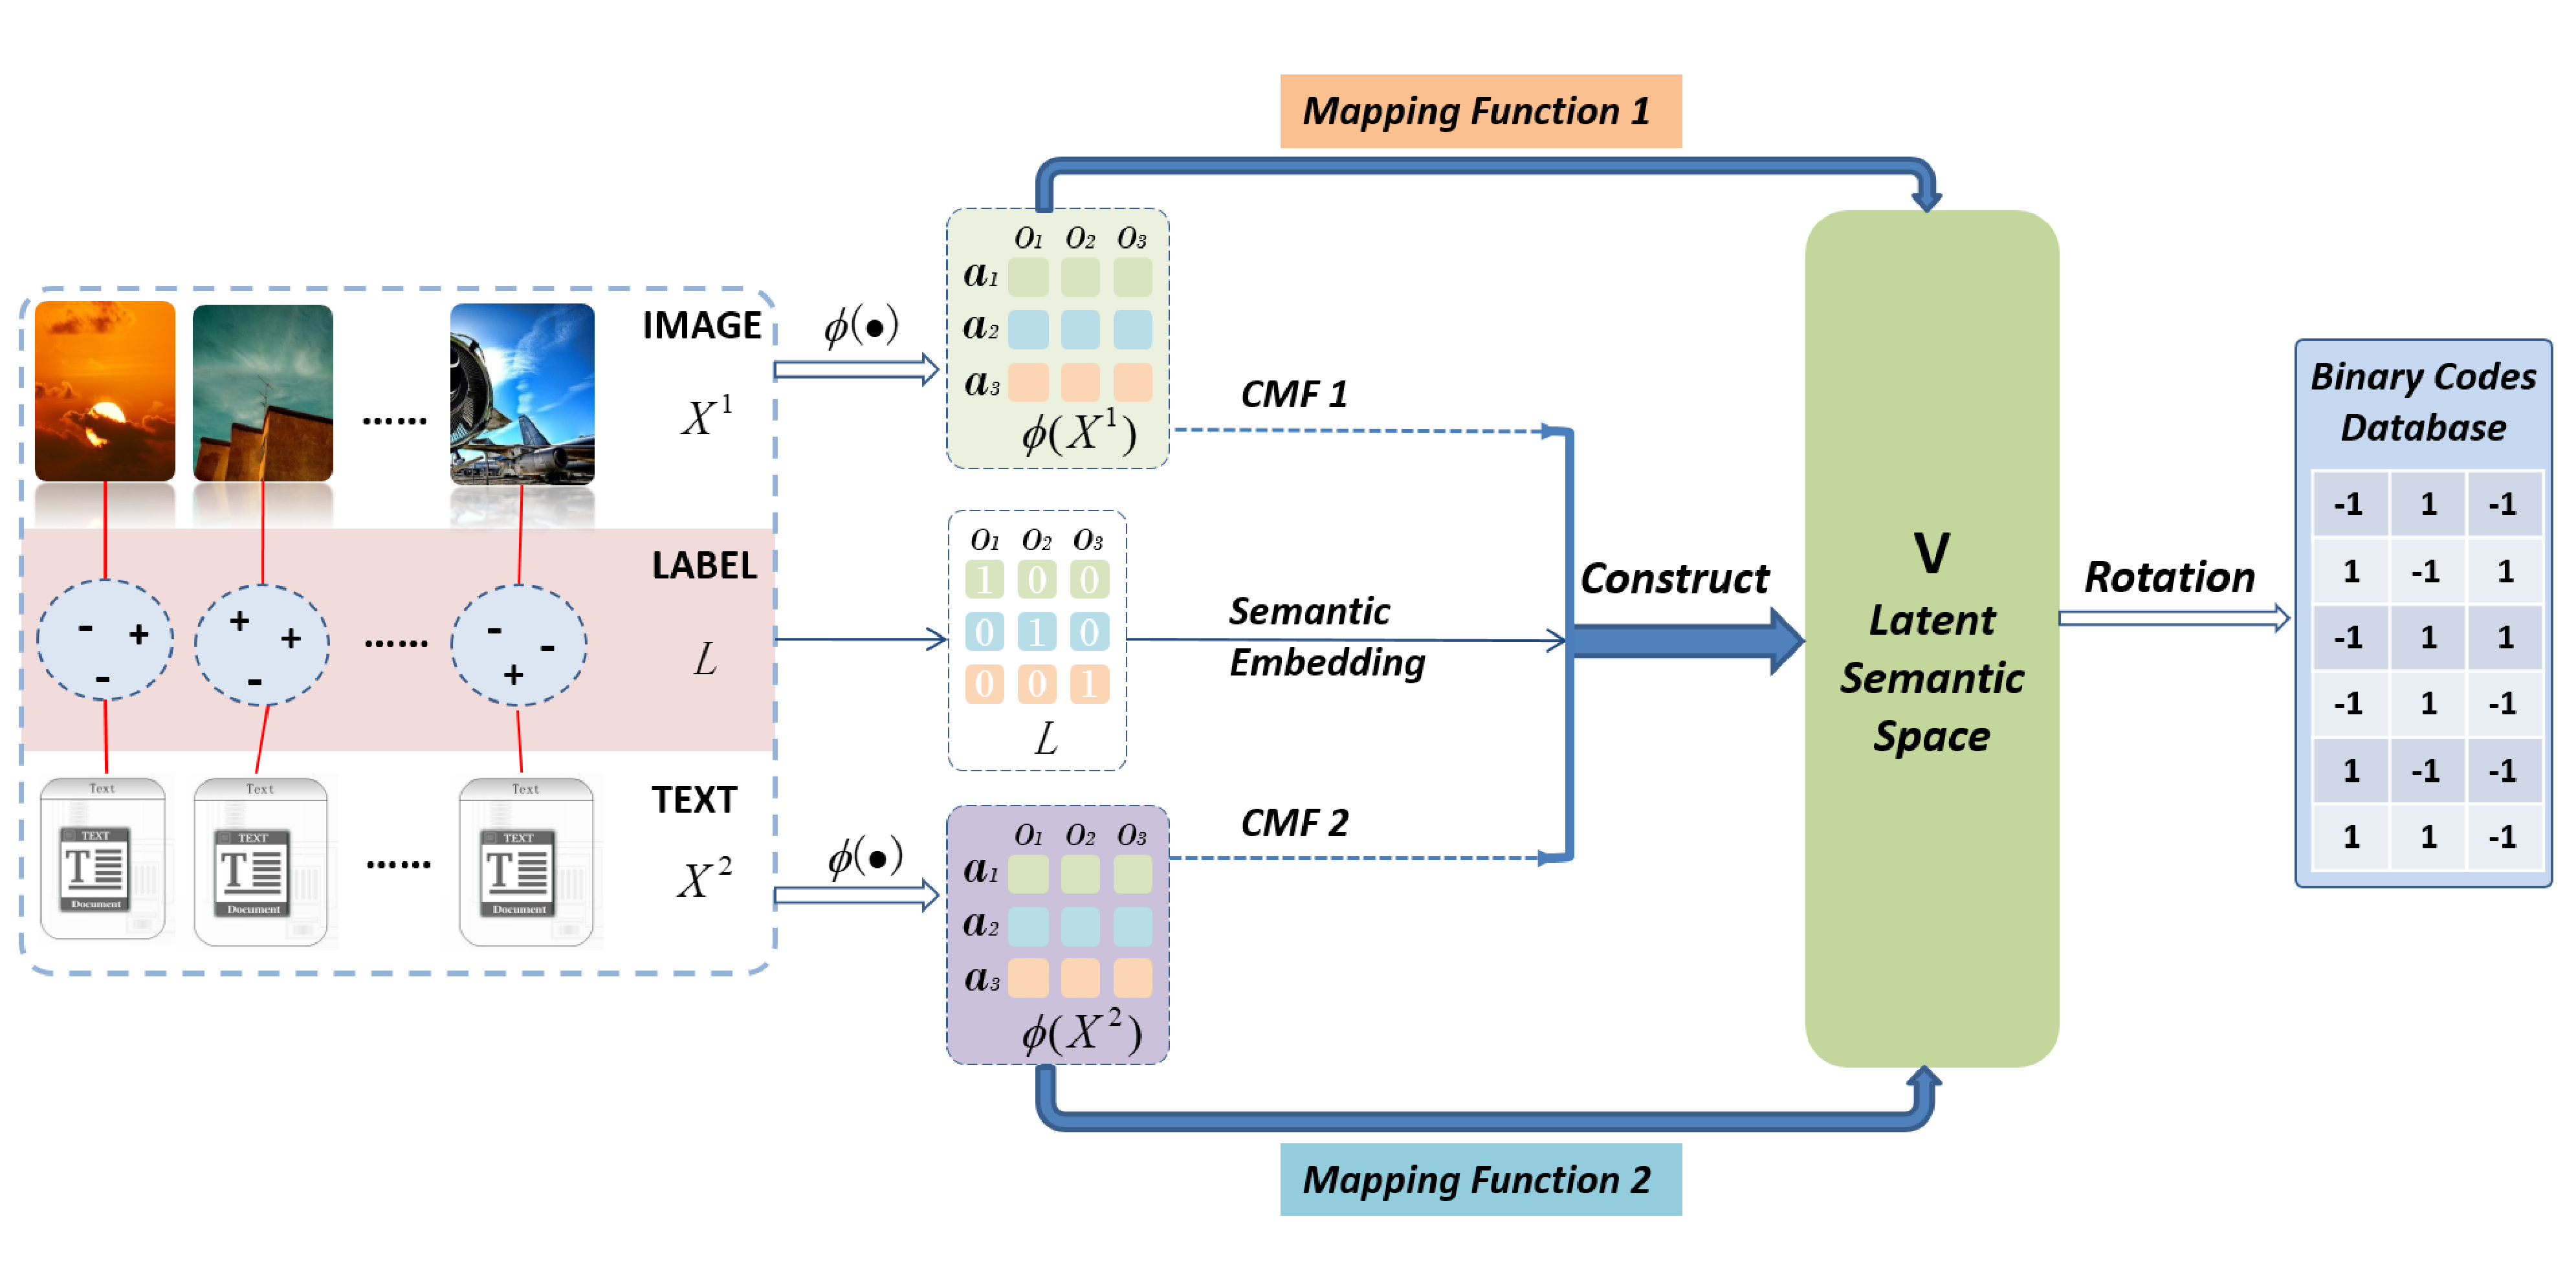
\includegraphics[width=0.97\textwidth]{figures/pipeline.eps}
\caption{SCRATCH������ͼ}
\label{pipeline}
\end{figure}


\section{�Ż�����}
\esection{Optimization process}

����֤����ʽ \ \eqref{obj} �е��Ż����������\ $\textbf{U}_t$��$\textbf{P}_t$��$\textbf{G}$��$\textbf{V}$��$\textbf{R}$ ��\ $\textbf{B}$ ֮���Ƿ�͹��ϵ���⵼�������Ż���������Ž������Ϊ\ NP-hard �����������⡣���˵��ǣ����̶��������������ֻ�Ż�����һ���������ʱ�����Ż�������þ�������dz�͹��ϵ�ģ����Ϊ�˽����ʽ\ \eqref{obj} �е��Ż����⣬SCRATCH �����һ�ֵ��������Ż����ԣ���ÿ�ι̶�������������������Ż�һ��������������ڿ��Եõ��þ�������ı�ʽ�⣬��˸��Ż����Ե�ѵ���ٶȿ�����������������٣�������Ż��������£�

%\vspace{1mm}
\textbf{��һ�����̶������������������\ $\textbf{U}_t$.}

��������������̶�ʱ��Ŀ�꺯��\ \eqref{obj} �ɱ���дΪ��
\begin{equation}
\label{obj-1}
    \min_{\textbf{U}_t} \lambda_t\parallel \bm{\phi}(\textbf{X}^{(t)})-\textbf{U}_t\textbf{V} \parallel^2_F+\gamma \parallel \textbf{U}_t \parallel^2_F.
\end{equation}

����ʽ\ \eqref{obj-1} ����\ $\textbf{U}_t$ �ĵ�����Ϊ�㣬���Եõ����¹���\ $\textbf{U}_t$ �ı�ʽ�⣺
\begin{equation}
\label{solveUt}
    \textbf{U}_t = \lambda_t \bm{\phi}(\textbf{X}^{(t)})\textbf{V}^{\top}(\lambda_t \textbf{V}\textbf{V}^{\top}+\gamma \textbf{I})^{-1}.
\end{equation}

%\vspace{4mm}
\textbf{�ڶ������̶������������������\ $\textbf{G}$.}

��\ $\textbf{U}_t$ ����������ͬ����������������̶�ʱ����ʽ\ \eqref{obj} �ɱ���дΪ��
\begin{equation}
\label{obj-2}
    \min_{\textbf{G}} \alpha \parallel \textbf{L}-\textbf{G}\textbf{V} \parallel^2_F+\gamma \parallel \textbf{G} \parallel^2_F.
\end{equation}

ͬ������ʽ\ \eqref{obj-2} ����\ $\textbf{G}$ �ĵ�����Ϊ�㣬���ǿ����Ƶ�������\ $\textbf{G}$ �Ľ��������£�
\begin{equation}
\label{solveUL}
    \textbf{G} = \alpha \textbf{L}\textbf{V}^{\top}(\alpha \textbf{V}\textbf{V}^{\top}+\gamma \textbf{I})^{-1},
\end{equation}

����\ $\textbf{I} \in \mathbb{R}^{r \times r}$ ��һ����λ����

%\vspace{1mm}
\textbf{���������̶������������������\ $\textbf{P}_t$.}

��������������̶�ʱ����ʽ\ \eqref{obj} �ɸ�дΪ��
\begin{equation}
\label{obj-3}
    \min_{\textbf{P}_t} \mu \parallel \textbf{V}-\textbf{P}_t\bm{\phi}(\textbf{X}^{(t)}) \parallel^2_F + \gamma \parallel \textbf{P}_t \parallel^2_F.
\end{equation}

ͨ������ʽ\ \eqref{obj} ����\ $\textbf{P}_t$ �ĵ�����Ϊ��ɵã�
\begin{equation}
\label{solvePt}
    \textbf{P}_t = \mu \textbf{V} \bm{\phi}(\textbf{X}^{(t)})^{\top} \Big(\mu \bm{\phi}(\textbf{X}^{(t)}) \bm{\phi}(\textbf{X}^{(t)})^{\top}+\gamma \textbf{I} \Big)^{-1}.
\end{equation}

\textbf{���IJ����̶������������������\ $\textbf{V}$.}

��ǰ����һ�����̶������������ͬʱ����ʽ\ \eqref{obj} ��дΪ��
\begin{equation}
\label{obj-4}
    \begin{split}
        &\min_{\textbf{V}} \sum_{t=1}^m \lambda_t \parallel \bm{\phi}(\textbf{X}^{(t)})-\textbf{U}_t\textbf{V} \parallel^2_F +\mu \sum_{t=1}^m \parallel \textbf{V}-\textbf{P}_t\bm{\phi}(\textbf{X}^{(t)}) \parallel^2_F\\
        &\ \ \ \ \ \ \ \ + \alpha \parallel \textbf{L}-\textbf{G}\textbf{V} \parallel^2_F+\parallel \textbf{B}-\textbf{R}\textbf{V} \parallel^2_F + \gamma \parallel \textbf{V} \parallel^2_F\\
    \end{split}
\end{equation}

����ʽ\ \eqref{obj-4} ����\ $\textbf{V}$ �ĵ�����Ϊ��ɵã�
\begin{equation}
\label{solveV}
    \begin{split}
    &\textbf{V} = \Big ( \sum_{t=1}^m \lambda_t \textbf{U}_t^{\top} \textbf{U}_t+\alpha \textbf{G}^{\top}\textbf{G} +  \textbf{R}^{\top}\textbf{R}+( m\mu+\gamma)\textbf{I} \Big) ^{-1}\bullet\\
    & \ \ \ \ \ \ \Big(\sum_{t=1}^m \big( \lambda_t \textbf{U}_t^{\top} \bm{\phi}(\textbf{X}^{(t)})+ \mu \textbf{P}_t \bm{\phi}(\textbf{X}^{(t)}) \big)+\alpha \textbf{G}^{\top}\textbf{L}+ \textbf{R}^{\top}\textbf{B} \Big). \\
    \end{split}
\end{equation}


\textbf{���岽���̶������������������\ $\textbf{R}$.}

�̶�������������󣬹�ʽ\ \eqref{obj} �ɱ���дΪ��
\begin{equation}
\label{solveR_eq}
    \begin{split}
        &\min_\textbf{R}\parallel \textbf{B}-\textbf{R}\textbf{V}\parallel^2_F, \\
        &s.t. \ \ \ \textbf{R}\textbf{R}^{\top}=\textbf{I}.
    \end{split}
\end{equation}

����������һ�����������\ Procrustes ����\ \cite{Sch1966OPP}���������ɽ�������ֵ�ֽ⣨SVD�����������˿ɵõ�\ $\textbf{B}\textbf{V}^\top=\textbf{S}\bm{\Omega}\bm{\widetilde{S}}^\top$��Ȼ�󽫹�ʽ\ \eqref{solveR_eq} չ���ɵã�
\begin{equation}
\label{solveR-1}
    \begin{split}
        &\min_\textbf{R} \parallel\textbf{B}\parallel^2_F-2Tr(\textbf{R}\textbf{V}\textbf{B}^{\top})+\parallel\textbf{R}\parallel^2_F), \\
        &s.t. \ \ \ \textbf{R}\textbf{R}^{\top}=\textbf{I}.
    \end{split}
\end{equation}

��Լ��\ $\textbf{R}\textbf{R}^{\top}=\textbf{I}$ ��֪��$\parallel\textbf{R}\parallel^2_F= Tr(\textbf{V}^{\top}\textbf{R}^{\top}\textbf{R}\textbf{V})=Tr(\textbf{V}\textbf{V}^{\top})$����$\parallel\textbf{B}\parallel^2_F=Tr(\textbf{B}\textbf{B}^{\top})$=������������ֵ�ֽ�ɵã�$Tr(\textbf{R}\textbf{V}\textbf{B}^{\top})=Tr(\textbf{B}\textbf{V}^{\top}\textbf{R}^{\top})=Tr(\textbf{S}\bm{\Omega}\bm{\widetilde{S}}^\top\textbf{R}^{\top})=Tr(\bm{\Omega}\bm{\widetilde{S}}^\top\textbf{R}^{\top}\textbf{S})$����˹�ʽ\ \eqref{solveR-1} ����дΪ��
\begin{equation}
\label{solveR-2}
    \begin{split}
        &\max_\textbf{R} Tr(\bm{\Omega}\bm{\widetilde{S}}^\top\textbf{R}^{\top}\textbf{S}), \\
        &s.t. \ \ \ \textbf{R}\textbf{R}^{\top}=\textbf{I}.
    \end{split}
\end{equation}

��\ Von Neumann ������ʽ \cite{mirsky1975trace} ��֪����������˵ļ�С�ڵ�����������Զ�Ӧ������ֵ���֮�ͣ���$Tr\big(\bm{\Omega}\bm{\widetilde{S}}^\top\textbf{R}^{\top}\textbf{S}\big)\le \sum_{i=1}^r \sigma_i\big(\bm{\Omega}\big)\sigma_i\big(\bm{\widetilde{S}}^\top\textbf{R}^{\top}\textbf{S}\big)$������\ $\sigma_i(\textbf{X})$ ����ȡ����\ $\textbf{X}$ �ĵ�\ $i$ ������ֵ�������ھ���\ $\bm{\widetilde{S}}$ ��\ $\textbf{S}$ ��Ϊ�Ͼ������\ $\bm{\widetilde{S}}^\top\textbf{R}^{\top}\textbf{S}\big(\bm{\widetilde{S}}^\top\textbf{R}^{\top}\textbf{S}\big)^\top=\bm{\textbf{I}}$����\ $\forall_i\sigma_i\big(\bm{\widetilde{S}}^\top\textbf{R}^{\top}\textbf{S}\big)=1$���ɵã�$Tr\big(\bm{\Omega}\bm{\widetilde{S}}^\top\textbf{R}^{\top}\textbf{S}\big)\le \sum_{i=1}^r \sigma_i\big(\bm{\Omega}\big)$��ֻ�е�\ $\textbf{R}=\bm{\textbf{S}\widetilde{S}}^\top$ ʱ�Ⱥų��������Կ����Ƶ��ó�\ $\textbf{R}$ �Ľ�����Ϊ\ \ $\textbf{R}=\bm{\textbf{S}\widetilde{S}}^\top$��

%\vspace{1mm}
\textbf{���������̶������������������\ $\textbf{B}$.}

��������������̶�ʱ����ʽ\ \eqref{obj} ��дΪ��
\begin{equation}
\label{solveB_eq}
    \begin{split}
        &\min_\textbf{B}\parallel \textbf{B}-\textbf{R}\textbf{V}\parallel^2_F,\\
        &s.t. \ \ \ \textbf{B}\in \{-1,1\}^{r \times n}.
    \end{split}
\end{equation}

��Ȼ���Կ�����������������Ž�Ϊ\ $\textbf{B}=sgn(\textbf{R}\textbf{V})$���Ҹ��������й�ϣ�����ʼ�ձ�����ɢ���Զ�δ�����ɳ��Ż�������̶��ϼ�С��������ͬʱ��������ɵĹ�ϣ��������ʹ�ü������ܴ����ߡ�

Ϊ�˻���Ż�Ŀ��\ \eqref{obj} �����Ž⣬����ͨ��������������Ż�\ $\textbf{U}_t$, $\textbf{G}$, $\textbf{P}_t$, $\textbf{V}$, $\textbf{R}$ ��\ $\textbf{B}$ ֱ��Ŀ��������Ŀ�꺯��ֵС����ֵ����������ﵽ�̶���������Ϊ�˸�������������������ĵ����Ż����ԣ�������\textbf{Algorithm 1}�������ܽᡣ
\begin{algorithm}[t]
   \caption{SCRATCH�Ż��㷨}
  \label{alg:example}
\begin{algorithmic}
   \STATE {\bfseries ���룺} ��$t$��ģ̬��ѵ�����ݾ���\ $\textbf{X}^{(t)}$��ƽ�����$\lambda_t$��$\mu$�� $\alpha$��$\gamma$����ϣ�볤��\ $r$ ���ܵ�������\ $c$.
   \STATE {\bfseries �����} ��ϣ�����\ $\textbf{B}$��ӳ�����\ $\textbf{P}_t$��$\textbf{G}$���ֽ����\ $\textbf{U}_t$����ת����\ $\textbf{R}$ ������������ʾ����\ $\textbf{V}$.
%   \vspace{-3mm}
   \STATE {\bfseries ���̣�}\\
     1. �����ʼ���������\ $\textbf{B}$��$\textbf{R}$��$\textbf{V}$��$\textbf{U}_t$��$\textbf{G}$ ��\ $\textbf{P}_t$��\\
     2. ��\ $\textbf{X}^{(t)}$ Ƕ�뵽�����Ժ˿ռ��в���ú˻��������\ $\textbf{F}_t(\textbf{X}^{(t)})$��\\
   \FOR {$i=1$ to $c$ }
   \STATE 3. �̶� $\textbf{P}_t$��$\textbf{G}$��$\textbf{V}$��$\textbf{R}$ �� $\ \textbf{B}$��ʹ�ù�ʽ\ \eqref{solveUt} ����\ $\textbf{U}_t$ ��\\
   4. �̶� $\textbf{U}_t$��$\textbf{P}_t$��$\textbf{V}$��$\textbf{R}$ �� $\ \textbf{B}$, ʹ�ù�ʽ\ \eqref{solveUL} ����\ $\textbf{G}$��\\
   5. �̶� $\textbf{U}_t$��$\textbf{G}$��$\textbf{V}$��$\textbf{R}$ �� $\ \textbf{B}$, ʹ�ù�ʽ\ \eqref{solvePt} ����\ $\textbf{P}_t$��\\
   6. �̶� $\textbf{U}_t$��$\textbf{G}$��$\textbf{P}_t$��$\textbf{R}$ �� $\ \textbf{B}$, ʹ�ù�ʽ\ \eqref{solveV} ����\ $\textbf{V}$��\\
   7. �̶� $\textbf{U}_t$��$\textbf{G}$��$\textbf{P}_t$��$\textbf{V}$ �� $\ \textbf{B}$, ʹ�ù�ʽ\ $\textbf{R}=\bm{\textbf{S}\widetilde{S}}^\top$ ����\ $\textbf{R}$��\\
   8. �̶� $\textbf{U}_t$��$\textbf{G}$��$\textbf{P}_t$��$\textbf{V}$ �� $\ \textbf{R}$, ʹ�ù�ʽ\ $sgn(\textbf{R}\textbf{V})$ ����\ $\textbf{B}$��\\
   \ENDFOR
   \STATE {\bfseries ����} $\textbf{U}_t$��$\textbf{P}_t$��$\textbf{G}$��$\textbf{V}$��$\textbf{R}$ �� $\ \textbf{B}$.
\end{algorithmic}
\end{algorithm}


\section{�㷨����}
\esection{Algorithm analysis}

\subsection{��������չ}
\esubsection{Out-of-sample extension}

����һ������ѵ�����е���������˵��SCRATCH ���Կ��ٵ����ɸ������Ĺ�ϣ�롣���磬����ij������ѯ��ģ̬�����е�һ��ģ̬����\ $\textbf{x}^{(t)}$������Ӧ�Ĺ�ϣ��������¹�ʽ�����ɣ�
%\vspace{-1mm}
\begin{equation}
    \textbf{b}^{(t)}=sgn\big(\textbf{R}\textbf{F}_t(\bm{\phi}(\textbf{x}^{(t)}))\big)=sgn\big(\textbf{R} \textbf{P}_t \bm{\phi}(\textbf{x}^{(t)})\big),
\end{equation}

����\ $\bm{\phi}(\textbf{x}^{(t)})$ ������\ $\textbf{x}^{(t)}$ �ķ�����Ƕ��˺�����


\subsection{ʱ�临�Ӷȷ���}
\esubsection{Time complexity analysis}

�ڱ�С���У�����չʾ��\ SCRATCH �Ż�������ʱ�临�Ӷ���ѵ������ģ�����Թ�ϵ���Ӷ�ʹ��\ SCRATCH �ڴ��ģ���ݼ��ϵĶ�ģ̬���ݼ���������Ϊ���ݹ�ģ������ѵ�����Ӷȵ���������˾��и߿���չ�Ժ�ʵ���ԡ�������˵�������ʱ�临�Ӷȷֱ������⹫ʽ\ \eqref{solveUt} ���ĵ�$O\big(c((qr + r^2)n + r^3 + qr^2)\big)$�����ڹ�ʽ\ \eqref{solveUL} ��$O\big(c((lr + r^2)n + r^3 + lr^2)\big)$�� ���\ \eqref{solvePt} ��$O\big(c((qr+q^2)n + q^3 + rq^2)\big)$�����ڹ�ʽ\ \eqref{solveV} ��$O\big(c(mqr^2+lr^2+2r^3+r(l+r+mq)n)\big)$����\ $\textbf{R}$ �Ľ���������$O\big(c(r^2n+r^3)\big)$�Լ����\ $\textbf{B}$ ��$O\big(c(r^2+r)n\big)$������\ $q$ �����ѡȡ��ê��������$r$ �ǹ�ϣ�볤�ȣ�$l$ �����������$m$ ��ģ̬������$c$ �ǵ�������������\ $r, l, q, m, c << n$�����ѵ���׶������������㸴�Ӷ�Ϊ$O(n(r^2+lr+q^2+mqr)c)$���ɼ�����ѵ�������ݹ�ģ\ $n$ �dz����Թ�ϵ�ġ���С�ڣ�2.4.1����֪�������׶����ɴ���ѯ������ϣ���ʱ�临�Ӷ�Ϊ$O(qr)$��ͬʱͨ�������½ڵ�ʵ���֪��SCRATCH ��ѵ���ͼ����ٶȶ��ǵ�ǰ��ģ̬��ϣ�����������ٶȺͼ�������ƽ����õķ�����

\subsection{��������}
\esubsection{Theorem analysis}

����1�����ݾ���ֽ��ϣ��CMFH��\cite{ding14cmfh}����ʽ\ \eqref{mf_info} �е�Эͬ����ֽ��빫ʽ\ \eqref{mapping} �е�����ӳ�����Ͽ�ʵ�������Ա������ԡ�

֤�������ݹ�ʽ\ \eqref{obj}������ÿ��ģ̬\ $t$ ������\ $i$��ͨ�������ع����\ $e_i^{(t)}$ ��\ $e_i^{'(t)}$���ɵ����¹�ʽ��
\begin{equation}
\label{proof-1}
    \begin{split}
        & x_i^{(t)}=\textbf{U}_tv_i+e_i^{(t)},\\
        & v_i=\textbf{P}_tx_i^{(t)}+e_i^{'(t)}.
    \end{split}
\end{equation}

���ڹ�ʽ\ \eqref{proof-1}������\ $x_i$ ��ȥ����\ $x_j$ ��ģΪ��
\begin{equation}
\label{proof-2}
    \begin{split}
        &\parallel x_i^{(t)}-x_j^{(t)}-(e_i^{(t)}-e_j^{(t)})\parallel = \parallel \textbf{U}_t(v _i-v_j)\parallel,\\
        &\parallel v_i-v_j \parallel = \parallel \textbf{P}_t(x_i^{(t)}-x_j^{(t)})+(e_i^{'(t)}-e_j^{'(t)})\parallel.
    \end{split}
\end{equation}

����ģ�����ԣ�����������������\ $\textbf{U}$ ��\ $\textbf{V}$������\ $\parallel\textbf{U}\textbf{V}\parallel \le \parallel\textbf{U}\parallel \parallel\textbf{V}\parallel$ �Լ�\ $\parallel \textbf{U}+\textbf{V} \parallel \le \parallel \textbf{U} \parallel+ \parallel \textbf{V} \parallel$�������Ƶ������¹�ʽ��
\begin{equation}
\label{proof-3}
    \begin{split}
        &\parallel x_i^{(t)}-x_j^{(t)}-(e_i^{(t)}-e_j^{(t)})\parallel \le \parallel \textbf{U}_t\parallel \parallel v _i-v_j \parallel,\\
        &\parallel v_i-v_j \parallel \le \parallel \textbf{P}_t(x_i^{(t)}-x_j^{(t)})\parallel+\parallel e_i^{'(t)}-e_j^{'(t)}\parallel.
    \end{split}
\end{equation}

�������Եó����¹�ʽ���ۣ�
\begin{equation}
\label{proof-4}
    \begin{split}
        & \parallel v_i-v_j \parallel \ge C1 \parallel x_i^{(t)}-x_j^{(t)}\parallel-\epsilon_1^{(t)}(i,j),\\
        & \parallel v_i-v_j \parallel \le C2 \parallel x_i^{(t)}-x_j^{(t)}\parallel+\epsilon_2^{(t)}(i,j).
    \end{split}
\end{equation}

����\ $C1=max_t \frac{1}{\parallel \textbf{U}_t\parallel}$��$C2=min_t \frac{1}{\parallel\textbf{P}_t\parallel}$������֮�⣬�߽����\ $\epsilon_1^{(t)}(i,j)=\frac{\parallel e_i^{(t)}-e_j^{(t)}\parallel}{\parallel \textbf{U}_t\parallel}$��$\epsilon_2^{(t)}(i,j)=\parallel e_i^{'(t)}-e_j^{'(t)}\parallel$��

����\ $\epsilon_1=\{\epsilon_1^{(t)}(i,j);\forall t,i,j\}$ �� $\ \epsilon_2=\{\epsilon_2^{(t)}(i,j);\forall t,i,j\}$ ��Ϊ�߽����ϣ���ʽ\ \eqref{proof-4} ������\ $\parallel v_i-v_j \parallel$ �����±߽磬����ζ�Ź�ʽ\ \eqref{mapping} �е�ӳ�亯���ǽ���\ bi-Lipschitz �����ġ�Ȼ��\ $\epsilon^{(t)}$ ��ֵ��\ CMF ��ӳ�亯��Ӱ��ܴ󣬵�\ $\textbf{X}^{(t)}$ ��\ $\textbf{V}$ �������ֽ�ģ��������\ $\epsilon^{(t)}$ ����\ 0���ҵ�\ $x_i$ ��\ $x_j$ ��ԭʼ�ռ�����ʱ����ʽ\ \eqref{proof-4} �е����±߽������ᱣ֤\ $v_i$ ��\ $v_j$ Ҳ������ġ�

����������ͨ��Эͬ����ֽ�������ӳ�����ϣ���С����ʽ\ \eqref{mf_info} ��\ \eqref{mapping} ��ʵ�������Ա������ԡ�

%����2��\textbf{Algorithm 1}�е�ÿ�ε��������У���ʽ\ \eqref{obj}�е�Ŀ�꺯��ֵ�ǵ����ݼ��ġ�
%
%֤����

\section{������}
\esection{Summary}

�������ؽ�����\ SCRATCH �Ķ��塢��ʧ������ƺ��Ż����̣�ͬʱΪ�˸��õ����Ȿ������Ŀ�ģ̬��ϣ���������ǽ�һ���������㷨����չ��ʱ�临�Ӷ��Լ���ض�����ϵͳ�IJ�����\ SCRATCH �����ۻ����������������ʧ�������Ż����ԣ�SCRATCH ���������˹�ϣ��������Ա��ֺ���ɢ���ԣ�ͬʱ����������ʱ������ɴ��ģ���ݼ���ѵ�����Ӷ�ʹ�ø÷������м��ߵĿ���չ�Ժ�ʵ���ԡ�



\chapter{\quad\quad ʵ���������}
\label{chap3}
\echapter{Experimental Results and Analyses}

Ϊ����֤��������Ŀ�ģ̬��ϣ��������Ч�ԣ��������������õĻ�׼���ݼ���Wiki\cite{rasiwasia10wiki}��MIRFlickr-25K\cite{huiskes08mir} ��\ NUS-WIDE\cite{chua09nus}�������˽�һ������չʵ�飬����˸���ǰ�Ƚ���dz���ģ̬��ϣ������һ����ȿ�ģ̬��ϣ����������ʵ��Աȡ�ͬʱ��Ϊ�˸��õ�չʾ\ SCRATCH �������Աȷ�������Խ�ԣ�����ʹ��\ MAP ��������������ܣ���������ͬģ̬֮���໥������\ top-N precision ��\ precision-recall ��������һ��˵��\ SCRATCH ����ƶԿ�ģ̬�����������ܵľ޴�������



\section{���ݼ�}
\esection{Datasets}

\textbf{Wiki}�������ݼ��ɴ�\ Wikipedia �ռ���\ 2,866 ��ͼƬ-�ı��Թ��ɣ�����ʮ�����ÿ������ֻ����ʮ���е�һ�࣬���ڵ���ǩ���ݼ�������֮�⣬ÿ��������ͼƬģ̬��\ 128 ά��\ bag-of-visual SIFT ������������ʾ���ı�ģ̬��10ά�����������׷��䣨LDA��������������ʾ����������ݼ��У��������ѡȡ\ $75\%$ ��ͼƬ-�ı�����Ϊѵ�����ͼ�������ʣ���\ $25\%$ ��Ϊ����ѯ���Լ���

\textbf{MIRFlickr-25K}�������ݼ������˴�\ Flickr ���ռ���\ 25,000 ��ͼƬ��ÿ��ͼƬ��24����ͬ���ı���ǩ�е�һ�����������б�ǣ����ڶ��ǩ���ݼ�����ÿ������������һ����ǩ��ǡ�����ѡȡ���������ٰ���20���ı���ǵ�������Ϊʵ�����ݼ���������ѡȡ��\ 20,015 ��������ÿ��������ͼƬģ̬��\ 512 ά��\ GIST ������������ʾ���ı�ģ̬��\ 1,386 ά��\ bag-of-words ������ʾ���ڸ����ݼ��У��������ѡȡ\ 2,000 ��������Ϊ����ѯ���Լ��������\ 18,015 ������������Ϊѵ�����ͼ�������

\textbf{NUS-WIDE}: �����ݼ���\ Flickr ����ȡ��\ 269,648 ��ͼƬ��ÿ���������˹�������ṩ��\ 81 ����ǩ�е�һ��������Ҳ�Ƕ��ǩ���ݼ������ǵ�һЩ��ǩ�õıȽ�ϡ�٣�����ѡȡ��\ 10 ����õı�ǩ�����Ӧ��\ 186,577 ��ͼƬ��Ϊ���յ�ʵ�����ݼ���ÿ��ͼƬ-�ı��Ա����Ϊ\ 10 ���е�����һ�࣬����ÿ��ʵ��������ͼƬģ̬��ʾΪ\ 500 ά��\ bag-of-visual SIFT �����������ı�ģ̬����ʾΪ\ 1,000 ά���������������ڸ����ݼ����������ѡȡ\ 2,000 ��������Ϊ����ѯ���Լ���ʣ���\ 184,577 ��������Ϊѵ�����ͼ�������ֵ��һ����ǣ����ڸ����ݼ�������ģ�ϴ�ͨ�����ڲ��Թ�ϣ�����Ƿ����չ�����ģ���ݼ��ϡ�

\section{�Աȷ��������۱�׼}
\esection{Baselines and Metrics}

���ǽ�\ SCRATCH ����ֵ�ǰ�Ƚ���dz���ģ̬��ϣ��������LSSH\cite{zhouJ14LSSH}��CMFH\cite{ding14cmfh}��SCM-seq\cite{zhang14scm}��CCQ\cite{long16ccq}��SePH-km\cite{lin15seph}��SMFH\cite{Liu16smfh}��FSH\cite{liu17fsh} ��\ DCH\cite{xu17dch}���Լ�һ����ȿ�ģ̬��ϣ��������ȿ�ģ̬��ϣ��DCMH��\cite{jiang2017dcmh}������ʵ��Աȡ���Щ���������Ƿ�ʹ�üල��Ϣ�ɱ�����Ϊ���ࣺLSSH��CMFH��CCQ ��\ FSH ���޼ල��ģ̬��ϣ�������� SCM-seq��SePH-km��SMFH��DCH ��\ DCMH �����мල��ģ̬��ϣ���������жԱȷ�������������ԭ���������ṩ���ڴ˱�ʾ��ֿ��л������֮�⣬SCMFH\cite{ding2016scmfh} ��\ CMFH ���мල��չ�汾��Ȼ��\ SCMFH ԭ����\cite{ding2016scmfh} ����չʾ��ʵ������\ CMFH ��������������ԣ������ķ�����\ CMFH �м����������������\ SCMFH ��Դ������δ��������˱���δ��������Աȷ����С�

��������ض���Щģ�ͽ����˵���ѵ����չʾ����Щģ�����ܴﵽ����ý��������\ NUS-WIDE ���ݼ����ھ޴�SePH-km ��\ FSH ����ʹ����\ $n*n$ �������Ծ��������������������������������ӣ�Ϊ�˽����������������ĸ߶�������������⣬���ǽ�������\ CMFH\cite{ding14cmfh} ��\ SePH-km\cite{lin15seph} ��ʹ�õIJ��ԣ�ͨ����\ NUS-WIDE ѵ���������ѡȡ\ 5,000 ��������ѵ��\ SePH-km ��\ FSH���Ӷ���Сѵ�����ġ�SCRATCH �ĵ��ι��̲��ý�����֤��ѡȡ���ŵij����������ս��Ϊ��$\lambda_1=\lambda_2=0.5$��$\mu=1,000$��$ \alpha=500$��$\gamma=5$������֮�⣬�ܵ�����������Ϊ15 �Ρ�

���з��������ܾ�ʹ��\ Mean Average Precision (MAP)�����ж���������һ������ѯ����\ $\textbf{q}$ ��˵����ƽ�����ȣ�Average Precision��AP����ʾ���£�
\begin{equation}
	AP(q)= \frac{1}{L_q}\sum_{r=1}^nP_q(r)\delta_q(r),
\end{equation}

�����ݿ��У�$L_q$ ������\ $\textbf{q}$ ����ʵ����������$n$ �����ݿ�������������$P_q(r)$ �����˼���ǰ\ $r$ ��������׼ȷ�ʣ������\ $r$ ��������������ʵ���������Ļ�����\ $\delta_q(r)=1$������\ $\delta_q(r)=0$����\ Wiki ����ǩ���ݼ��ϣ���ʵ���ڱ�����Ϊ������ͬ��ǩ����Щ����������\ MIRFlickr-25K ��\ NUS-WIDE ���ݼ��ϣ����Ƕ�����ʵ����Ϊ��Щ���ٹ���һ�������ǩ����������ÿ���������ж����ǩ��ǣ�ֻҪ��һ����ǩ��ͬ����Ϊ���ڣ���

Mean Average Precision (MAP) ����Ϊ��ʽ��
\begin{equation}
	MAP=\frac{1}{|Q|}\sum_{i=1}^{|Q|} AP(q_i),
\end{equation}

����\ $|Q|$ ��������ѯ���Լ�������������


Ϊ�˸�ֱ�۵�չʾ\ SCRATCH �������Աȷ������������������������ǽ�һ�������˸������ݼ��Ϲ�ϣ��λ��Ϊ\ 64 λ��\ 128 λʱ��\ top-N precision ��\ precision-recall ���ߡ���ʵ���У�����̽����������ģ̬��������1) Image-to-Text��ʹ��ͼƬģ̬������Ϊ����ѯ������������Ӧ���ı�ģ̬���ݣ�2) Text-to-Image��ʹ���ı�ģ̬������Ϊ����ѯ������������Ӧ��ͼƬģ̬���ݡ��������еĶ�����׼��˵��MAP ֵԽ������������ڸ߶�Խ�ߣ�������÷���������Խ�á�


\begin{table}[htb]
\small
\center
\begin{center}
\caption{\bf Wiki ���ݼ�����\ MAP �����ܶԱ�}
\label{map_wiki}
%\vspace{-2mm}
\begin{tabular}{cllllll}
  \toprule[1pt]
  Task & Method & 8 bits & 16 bits & 32 bits & 64 bits & 128 bits\\
  \hline
  \multirow{8}{*}{\tabincell{c}{Image\\to\\Text}}
  & {LSSH} & {0.1831} & {0.2162} & {0.2164} & {0.2041} & {0.2084}\\
  & {CMFH} & {0.2006} & {0.2145} & {0.2288} & {0.2360} & {0.2396}\\
  & {SCM-seq} & {0.2125} & {0.2341} & {0.2410} & {0.2437} & {0.2541}\\
  & {CCQ} & {0.1642} & {0.1675} & {0.1683} & {0.1682} & {0.1680}\\
  & {SePH-km} & {0.2620} & {0.2796} &{0.2820} & {0.3076} & {0.3137}\\
  & {SMFH} & {0.1673} & {0.2276} & {0.2470} & {0.2955} & {0.3133}\\
  & {FSH} & {0.1992} & {0.2270} & {0.2433} & {0.2366} & {0.2463}\\
  & {DCH} & {0.3111} & {0.3491} & {0.3589} & {0.3777} & {0.3791}\\
  & {SCRATCH} & {\bf{0.3185}} & {\bf{0.3696}} & {\bf{0.3874}} & {\bf{0.4051}} & {\bf{0.4001}}\\
  \hline
  \multirow{8}{*}{\tabincell{c}{Text\\to\\Image}}
  & {LSSH} & {0.4268} & {0.4990} & {0.5225} & {0.5287} & {0.5330}\\
  & {CMFH} & {0.4434} & {0.4915} & {0.5252} & {0.5276} & {0.5347}\\
  & {SCM-seq} & {0.2013} & {0.2257} & {0.2459} & {0.2480} & {0.2530}\\
  & {CCQ} & {0.2094} & {0.2410} & {0.2518} & {0.2507} & {0.2543}\\
  & {SePH-km} & {0.6065} & {0.6379} & {0.6451} & {0.6662} & {0.6706}\\
  & {SMFH} & {0.3598} & {0.5242} & {0.5961} & {0.6608} & {0.6924}\\
  & {FSH} & {0.4092} & {0.4864} & {0.5197} & {0.4961} & {0.5247}\\
  & {DCH} & {0.6724} & {0.6815} & {0.7097} & {0.7216} & {0.7141}\\
  & {SCRATCH} & {\bf{0.7058}} & {\bf{0.7471}} &{\bf{0.7543}} & {\bf{0.7654}} &{\bf{0.7679}}\\
  \toprule[1pt]
\end{tabular}
\end{center}
\end{table}


\begin{figure*}
%\vspace{-12mm}
\begin{minipage}{0.5\linewidth}
\centering
\centerline{\includegraphics[width=8cm]{figures/Wiki_Precision/Precision_Image_VS_Text_64}}
\end{minipage}
%\vspace{-6mm}
\begin{minipage}{0.5\linewidth}
\centering
\centerline{\includegraphics[width=8cm]{figures/Wiki_Precision/Precision_Text_VS_Image_64}}
\end{minipage}
\caption{\bf Wiki ���ݼ�\ 64 λ��ϣ���\ Top-N precision ����}
\label{curves-wiki-1}\medskip
\end{figure*}

\begin{figure*}
\vspace{-12mm}
\begin{minipage}{0.5\linewidth}
\centering
\centerline{\includegraphics[width=8cm]{figures/Wiki_Precision/Precision_Image_VS_Text_128}}
\end{minipage}
%\vspace{-6mm}
\begin{minipage}{0.5\linewidth}
\centering
\centerline{\includegraphics[width=8cm]{figures/Wiki_Precision/Precision_Text_VS_Image_128}}
\end{minipage}
\caption{\bf Wiki ���ݼ�\ 128 λ��ϣ���\ Top-N precision ����}
\label{curves-wiki-2}\medskip
\end{figure*}



\begin{figure*}
\vspace{-12mm}
\begin{minipage}{0.5\linewidth}
\centering
\centerline{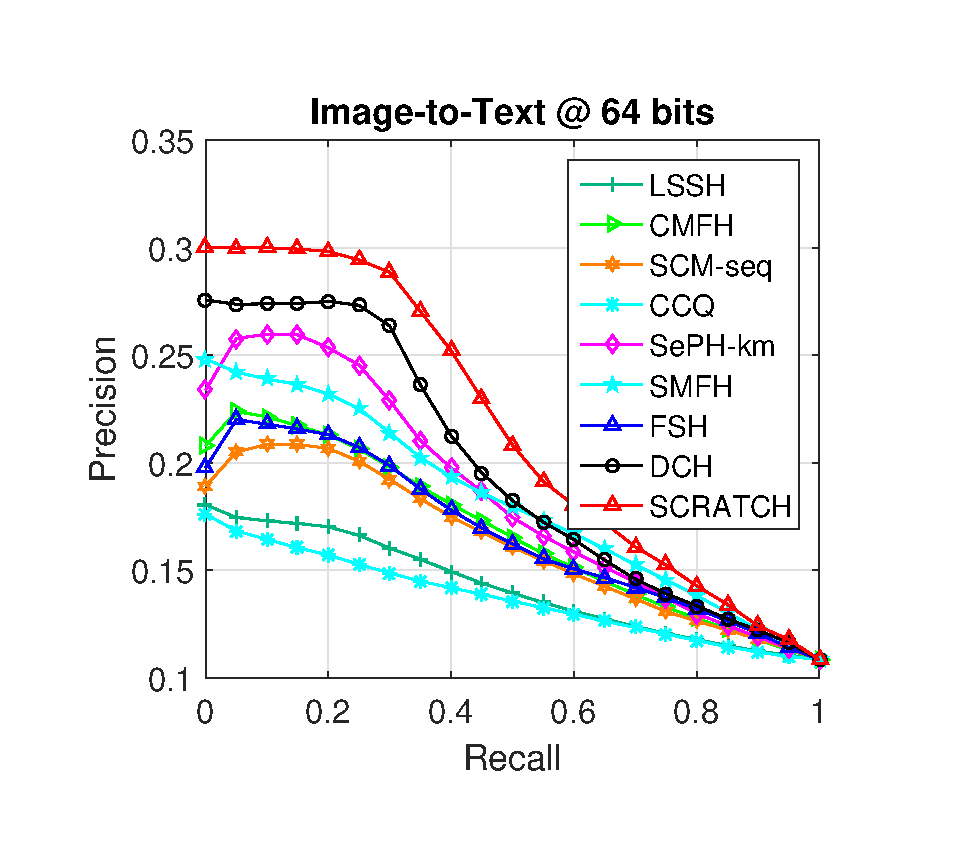
\includegraphics[width=8cm]{figures/WiKi_P_R/P_R_Image_Vs_Text_64}}
\end{minipage}
%\vspace{-6mm}
\begin{minipage}{0.5\linewidth}
\centering
\centerline{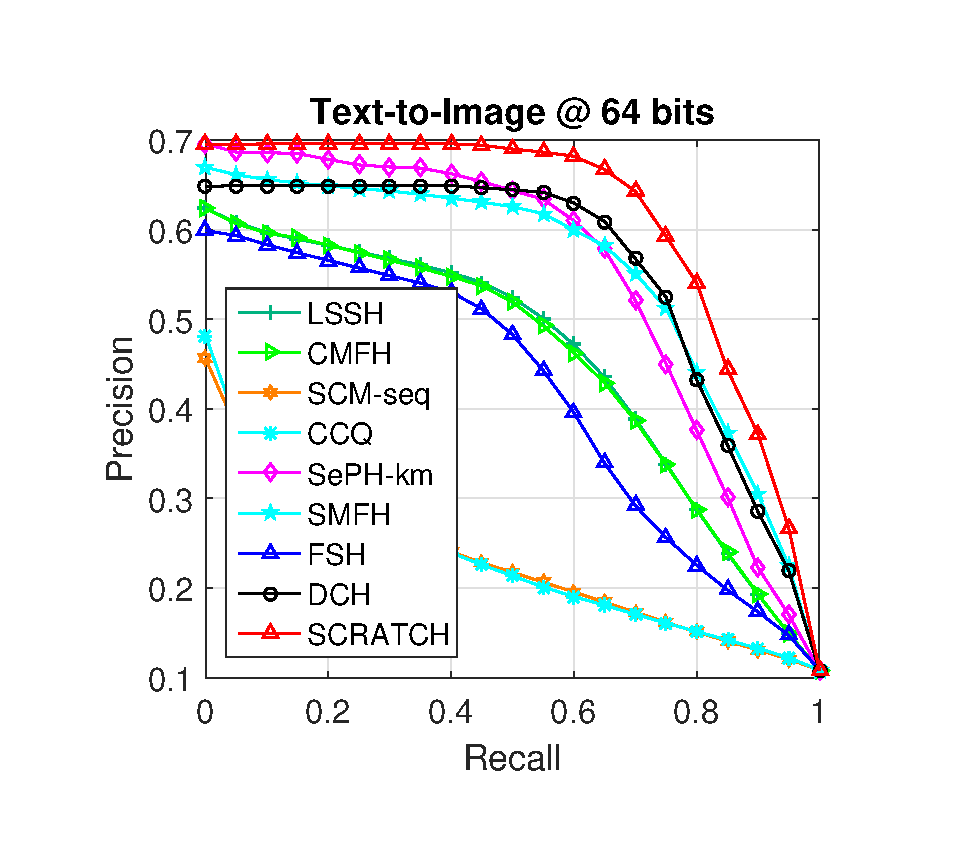
\includegraphics[width=8cm]{figures/WiKi_P_R/P_R_Text_Vs_Image_64}}
\end{minipage}
%\vspace{-4mm}
\caption{\bf Wiki ���ݼ�\ 64 λ��ϣ���\ Precision-Recall ����}
\label{curves-wiki-3}\medskip
\end{figure*}


\begin{figure*}
%\vspace{-12mm}
\begin{minipage}{0.5\linewidth}
\centering
\centerline{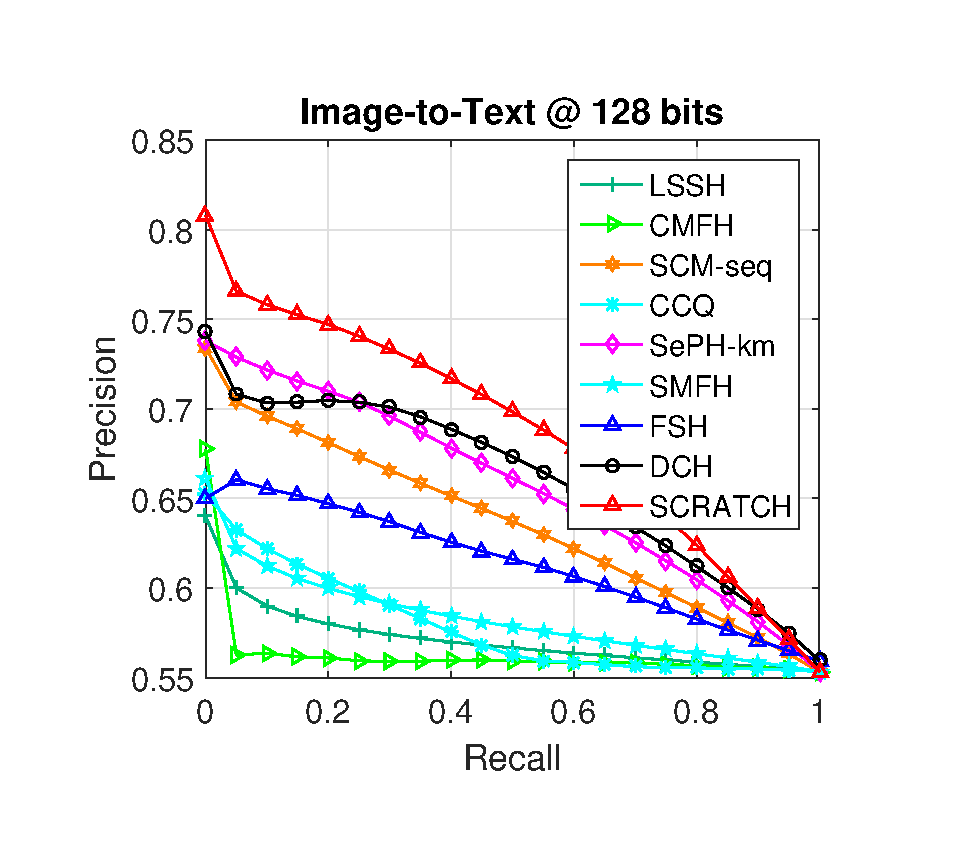
\includegraphics[width=8cm]{figures/Wiki_P_R/P_R_Image_Vs_Text_128}}
\end{minipage}
%\vspace{-6mm}
\begin{minipage}{0.5\linewidth}
\centering
\centerline{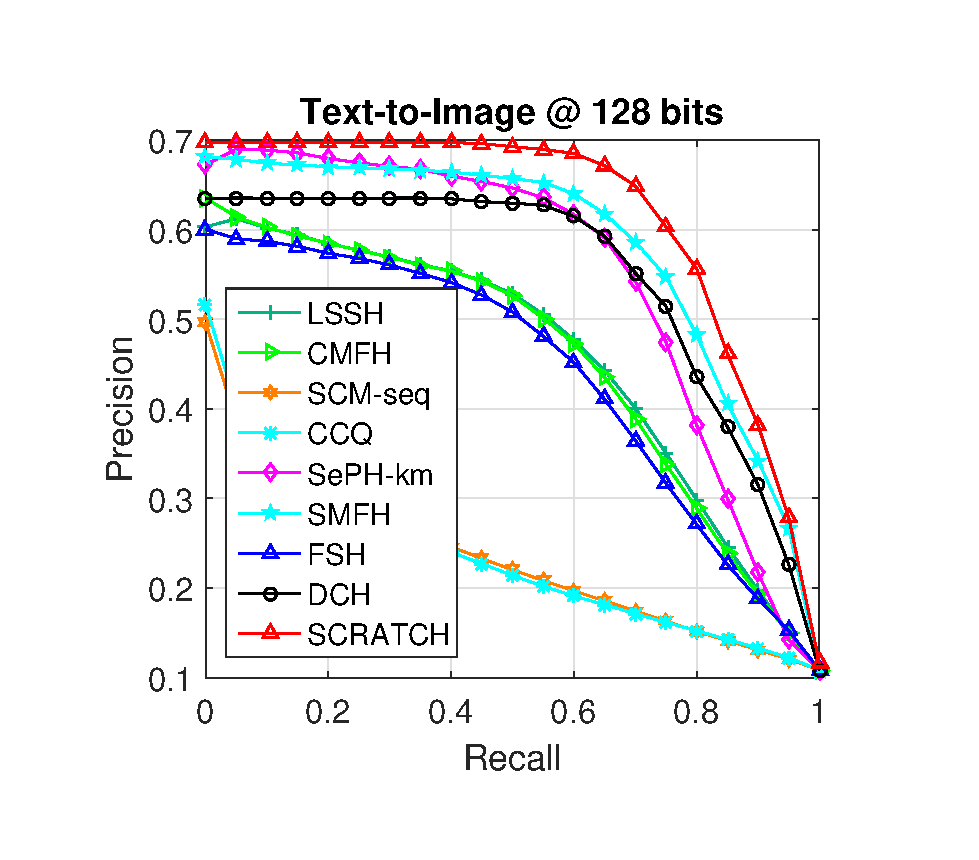
\includegraphics[width=8cm]{figures/WiKi_P_R/P_R_Text_Vs_Image_128}}
\end{minipage}
\caption{\bf Wiki ���ݼ�\ 128 λ��ϣ���\ Precision-Recall ����}
\label{curves-wiki-4}\medskip
\end{figure*}


\section{ʵ���������}
\esection{Results and Analysis}
\label{sec:result}
\subsection{Wiki ���ݼ�ʵ����}
\esubsection{Results on Wiki}
\label{sec:wiki}
SCRATCH �����жԱȷ�����\ Wiki ���ݼ��ϵ�\ MAP ʵ�����ڱ�\ \ref{map_wiki} �н���չʾ��Wiki ���ݼ���\ 64 λ��\ 128 λ��ϣ���ϵ�\ top-N precision ��\ precision-recall ������ͼ \ \ref{curves-wiki-1}��\ref{curves-wiki-4} �л���������Щ��������ǿ��Եó����¼�����ۣ�
%\leftmargini=7mm
%\leftmarginii=6mm
\begin{itemize}
\vspace{-3mm}
\item SCRATCH �ڸ�����ϣ��λ����ִ�����ֿ�ģ̬������������ܶ�Ҫ���������������жԱȷ�����
\vspace{-3mm}
\item ��\ Text-to-Image �����ϣ�SCRATCH ��\ MAP ����ҪԶԶ���������Աȷ��������������������Ҫԭ������������ͼ��ģ̬���ԣ�����ֽ�����״��ı�ģ̬�о�ȷ�ھ������������������Ϣ��
\vspace{-3mm}
\item �����мල��ģ̬��ϣ��������\ SCRATCH��DCH ��\ SePH-km��������ҪԶԶ��Խ�������޼ල��������\ CMFH ��\ FSH������һ��˵��������������Ϣ����Ҫ�ԡ�
\vspace{-3mm}
\item SCRATCH �� $N$ �dz�С��ʱ��Ҫ�������Աȷ������ָ��ã�������\ Image-to-Text �ϣ�����˵��\ SCRATCH ��\ $N$ ��Сʱ�ܹ������������ѯ��������ص����ݿ���������Լ���������˵�Ƿdz���Ҫ�ġ�
\end{itemize}


\begin{table}[htb]
\small
\center
\begin{center}
\caption{\bf MIRFlickr-25K ���ݼ�����\ MAP �����ܶԱ�}
\label{mAP_flickr}
%\vspace{-2mm}
\begin{tabular}{cllllll}
  \toprule[1pt]
  Task & Method & 8 bits & 16 bits & 32 bits & 64 bits & 128 bits\\
  \hline
  \multirow{8}{*}{\tabincell{c}{Image\\to\\Text}}
  & {LSSH} & {0.5698} & {0.5812} & {0.5811} & {0.5805} & {0.5800}\\
  & {CMFH} & {0.5599} & {0.5687} & {0.5680} & {0.5685} & {0.5687}\\
  & {SCM-seq} & {0.6235} & {0.6373} & {0.6478} & {0.6537} & {0.6611}\\
  & {CCQ} & {0.5712} & {0.5885} & {0.5908} & {0.5924} & {0.5928}\\
  & {SePH-km} & {0.6641} & {0.6685} &{0.6818} & {0.6830} & {0.6873}\\
  & {SMFH} & {0.5587} & {0.5688} & {0.5917} & {0.5953} & {0.5961}\\
  & {FSH} & {0.5911} & {0.6016} & {0.6149} & {0.6194} & {0.6242}\\
  & {DCH} & {0.6659} & {0.6738} & {0.6859} & {0.6897} & {0.7030}\\
  & {SCRATCH} & {\bf{0.7092}} & {\bf{0.7131}} &{\bf{0.7222}} & {\bf{0.7265}} &{\bf{0.7346}}\\
  \hline
  \multirow{8}{*}{\tabincell{c}{Text\\to\\Image}} %$T\rightarrow I$
  & {LSSH} & {0.5914} & {0.5917} & {0.5929} & {0.5926} & {0.5918}\\
  & {CMFH} & {0.5615} & {0.5615} & {0.5606} & {0.5606} & {0.5608}\\
  & {SCM-seq} & {0.6103} & {0.6206} & {0.6298} & {0.6372} & {0.6427}\\
  & {CCQ} & {0.5902} & {0.5970} & {0.5992} & {0.6001} & {0.6001}\\
  & {SePH-km} & {0.7033} & {0.7076} & {0.7212} & {0.7293} & {0.7348}\\
  & {SMFH} & {0.5568} & {0.5586} & {0.5727} & {0.5841} & {0.5828}\\
  & {FSH} & {0.5869} & {0.5979} & {0.6114} & {0.6186} & {0.6251}\\
  & {DCH} & {0.7256} & {0.7511} & {0.7585} & {0.7681} & {0.7909}\\
  %& {DCH} & {0.7344} & {0.7425} & {0.7599} & {0.7633} & {0.7927}\\
  & {SCRATCH} & {\bf{0.7591}} & {\bf{0.7762}} &{\bf{0.7822}} & {\bf{0.7978}} & {\bf{0.8063}}\\
  \toprule[1pt]
\end{tabular}
\end{center}
\end{table}

\subsection{MIRFlickr-25K ���ݼ�ʵ����}
\esubsection{Results on MIRFlickr-25K}
\label{sec:mirflickr}

MIRFlickr-25K ���ݼ���\ Image-to-Text ��\ Text-to-Image ������ģ̬���������\ MAP ʵ�����ڱ�\ \ref{mAP_flickr} �н������ܽᣬ�����ݼ���\ 64 λ��\ 128 λ��ϣ���ϵ�\ top-N precision ��\ precision-recall ������ͼ\ \ref{curves-flickr-1}��\ref{curves-flickr-4} �л�����ͨ������������\ MIRFlickr-25K ���ݼ��ϵ�ʵ���������ǿ��Թ۲쵽���漸�㣺
\begin{itemize}
\vspace{-3mm}
\item ����\ Wiki ���ݼ��ϵĽ����ͬ��SCRATCH �ڸ�����ϣ��λ����ִ�����ֿ�ģ̬������������ܶ�Ҫ���������������жԱȷ�����
\vspace{-3mm}
\item SCRATCH �ڹ�ϣ��λ���ܵͣ���\ 8 ��\ 16 λ����ʱ����Ȼȡ����Զ���������Աȷ����ļ������ܣ�����ζ�Ŷ��ڸ�ά������˵��SCRATCH ���Խ��併ά�����͵�ά�Ƚ��м�����ͬʱ��֤������������Ӷ�������������Ⱥ��ٶȡ�
\vspace{-3mm}
\item ���Ź�ϣ��λ�����ӣ�SCRATCH �ļ������ܳ���������˵�������Ĺ�ϣ���ܹ���������Ϣ�������ϣ���У��Ӷ�ʵ�ּ������ܵĿ���������
\vspace{-3mm}
\item һ����˵�������������\ Text-to-Image �����ϵļ�������ҪԶԶ����\ Image-to-Text ���񣬿��ܵ�ԭ�������ı���ͼ��������������������ı�-ͼ������������⣬�Ӷ�����ʹ���ı�������ͼ��������ס�
\vspace{-3mm}
\item ��\ Wiki ���ݼ��ϵ�ʵ������ȣ���\ MIRFlickr-25K ���ݼ������еķ�����ȡ���˸��õؼ������ܣ�������������������ݼ���ʹ�õ�������ʾ������ͬ��ͬʱ��ͬ�����ݼ������ݷֲ�Ҳ������ͬ��������ͬ�����ڲ�ͬ���ݼ��ϵļ��������������졣
\end{itemize}



\begin{figure*}
%\vspace{-12mm}
\begin{minipage}{0.5\linewidth}
\centering
\centerline{\includegraphics[width=8cm]{figures/FLICKR_Precision/Precision_Image_VS_Text_64}}
\end{minipage}
%\vspace{-6mm}
\begin{minipage}{0.5\linewidth}
\centering
\centerline{\includegraphics[width=8cm]{figures/FLICKR_Precision/Precision_Text_VS_Image_64}}
\end{minipage}
\caption{\bf MIRFlickr-25K ���ݼ�\ 64 λ��ϣ���\ Top-N precision ����}
\label{curves-flickr-1}\medskip
\end{figure*}


\begin{figure*}
\vspace{-6mm}
\begin{minipage}{0.5\linewidth}
\centering
\centerline{\includegraphics[width=8cm]{figures/FLICKR_Precision/Precision_Image_VS_Text_128}}
\end{minipage}
%\vspace{-6mm}
\begin{minipage}{0.5\linewidth}
\centering
\centerline{\includegraphics[width=8cm]{figures/FLICKR_Precision/Precision_Text_VS_Image_128}}
\end{minipage}
\caption{\bf MIRFlickr-25K ���ݼ�\ 128 λ��ϣ���\ Top-N precision ����}
\label{curves-flickr-2}\medskip
\end{figure*}


\begin{figure*}
%\vspace{-12mm}
\begin{minipage}{0.5\linewidth}
\centering
\centerline{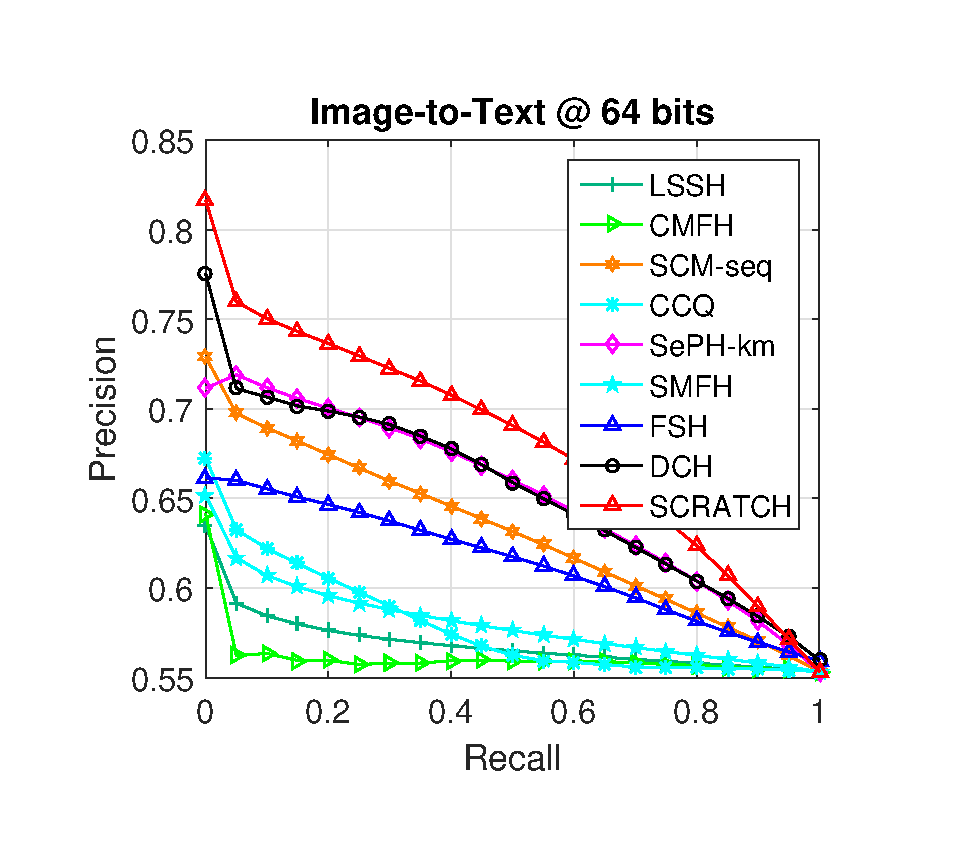
\includegraphics[width=8cm]{figures/FLICKR_P_R/P_R_Image_Vs_Text_64}}
\end{minipage}
%\vspace{-6mm}
\begin{minipage}{0.5\linewidth}
\centering
\centerline{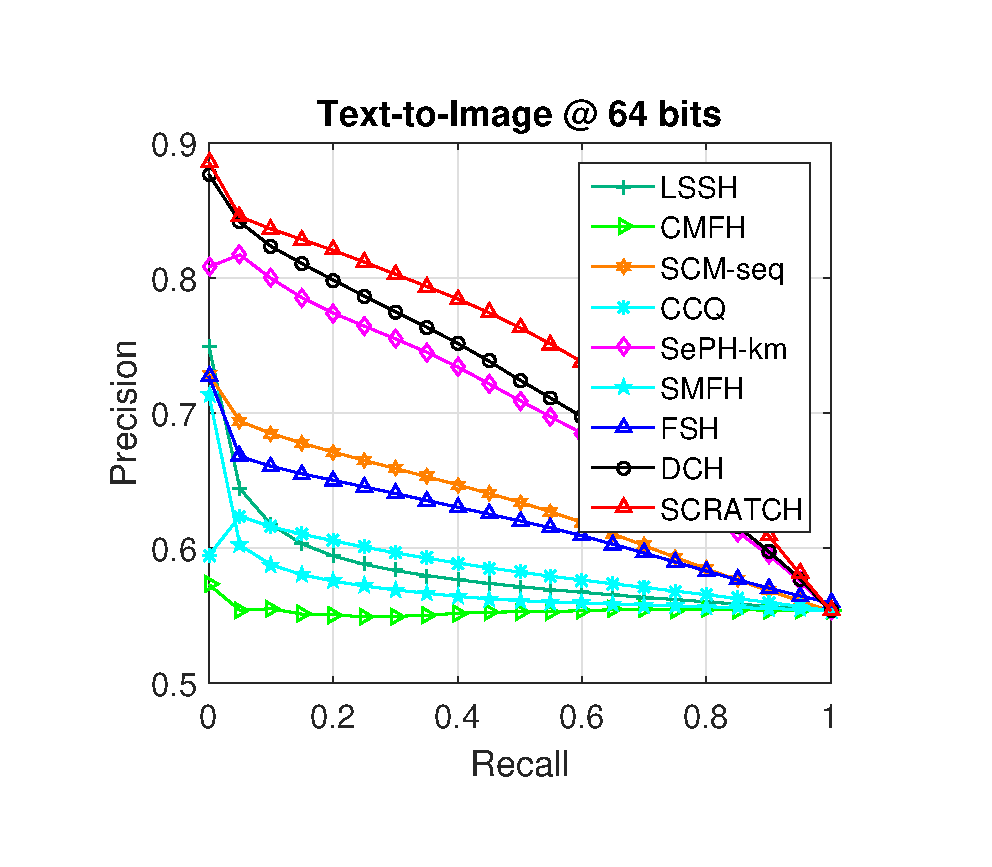
\includegraphics[width=8cm]{figures/FLICKR_P_R/P_R_Text_Vs_Image_64}}
\end{minipage}
%\vspace{-4mm}
\caption{\bf MIRFlickr-25K ���ݼ�\ 64 λ��ϣ���\ Precision-Recall ����}
\label{curves-flickr-3}\medskip
\end{figure*}


\begin{figure*}
\vspace{-12mm}
\begin{minipage}{0.5\linewidth}
\centering
\centerline{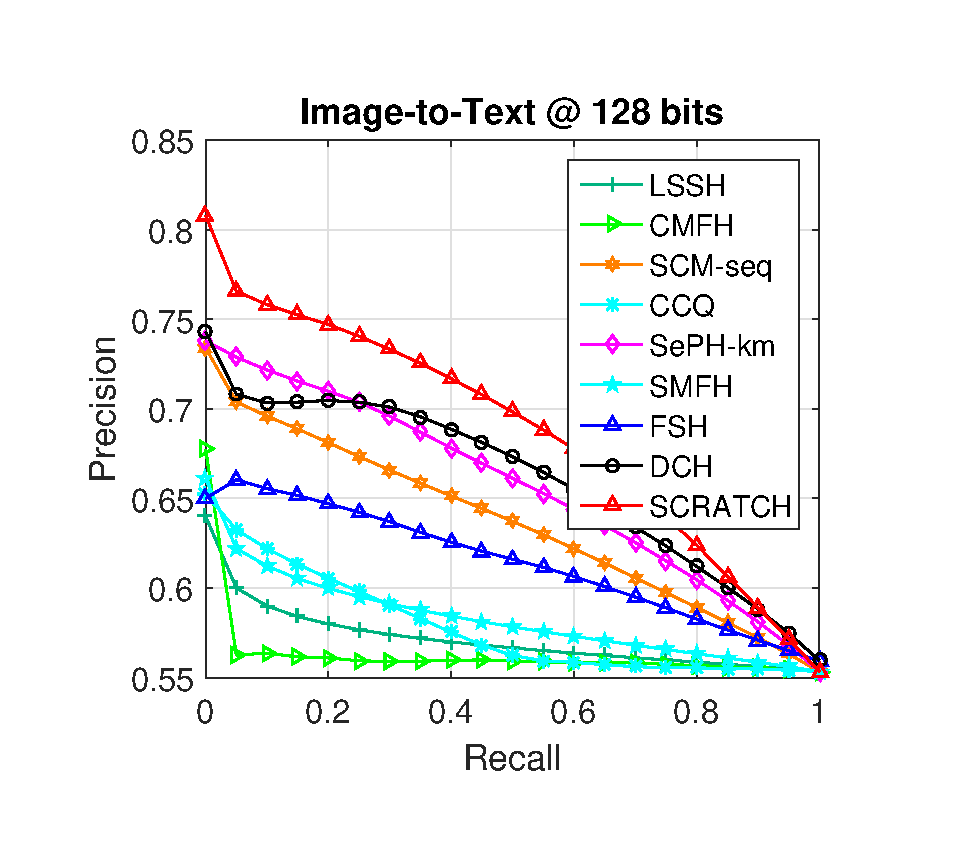
\includegraphics[width=8cm]{figures/Wiki_P_R/P_R_Image_Vs_Text_128}}
\end{minipage}
%\vspace{-6mm}
\begin{minipage}{0.5\linewidth}
\centering
\centerline{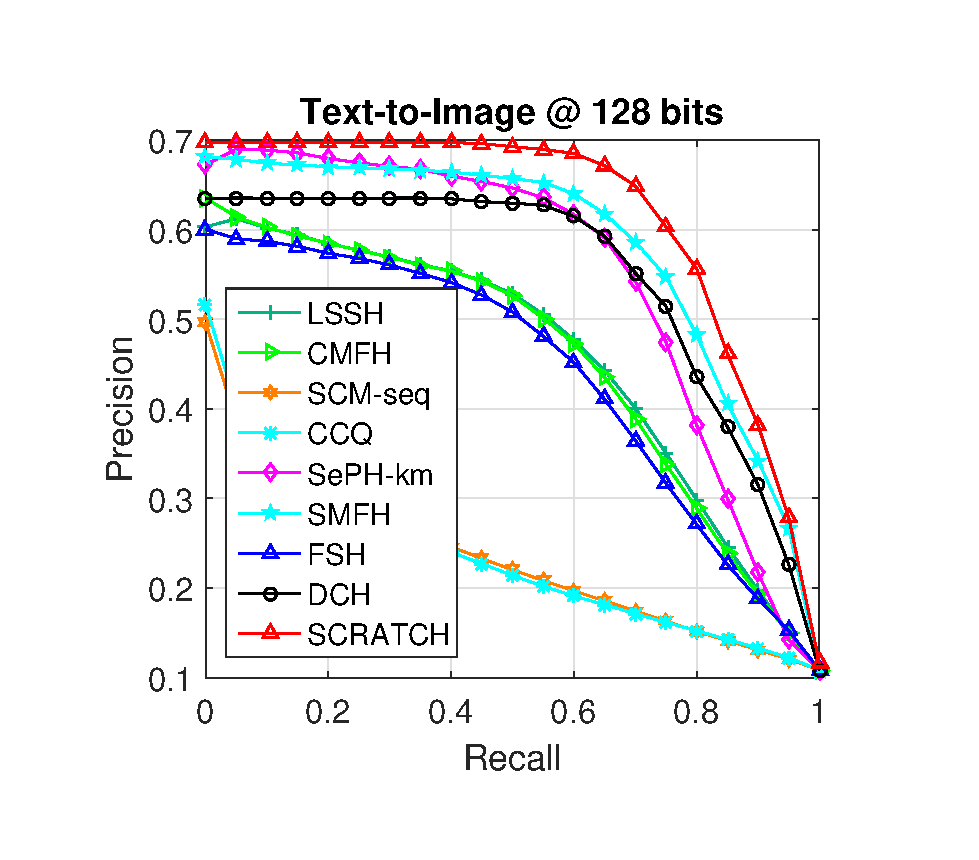
\includegraphics[width=8cm]{figures/WiKi_P_R/P_R_Text_Vs_Image_128}}
\end{minipage}
\caption{\bf MIRFlickr-25K ���ݼ�\ 128 λ��ϣ���\ Precision-Recall ����}
\label{curves-flickr-4}\medskip
\end{figure*}


\begin{figure*}
\vspace{-12mm}
\begin{minipage}{0.5\linewidth}
\centering
\centerline{\includegraphics[width=8cm]{figures/NUS_WIDE_Precision/Precision_Image_VS_Text_64}}
\end{minipage}
%\vspace{-6mm}
\begin{minipage}{0.5\linewidth}
\centering
\centerline{\includegraphics[width=8cm]{figures/NUS_WIDE_Precision/Precision_Text_VS_Image_64}}
\end{minipage}
\caption{\bf NUS-WIDE ���ݼ�\ 64 λ��ϣ���\ Top-N precision ����}
\label{curves-nus-1}\medskip
\end{figure*}

\begin{figure*}
%\vspace{-12mm}
\begin{minipage}{0.5\linewidth}
\centering
\centerline{\includegraphics[width=8cm]{figures/NUS_WIDE_Precision/Precision_Image_VS_Text_128}}
\end{minipage}
%\vspace{-6mm}
\begin{minipage}{0.5\linewidth}
\centering
\centerline{\includegraphics[width=8cm]{figures/NUS_WIDE_Precision/Precision_Text_VS_Image_128}}
\end{minipage}
\caption{\bf NUS-WIDE ���ݼ�\ 128 λ��ϣ���\ Top-N precision ����}
\label{curves-nus-2}\medskip
\end{figure*}



\begin{figure*}
\vspace{-12mm}
\begin{minipage}{0.5\linewidth}
\centering
\centerline{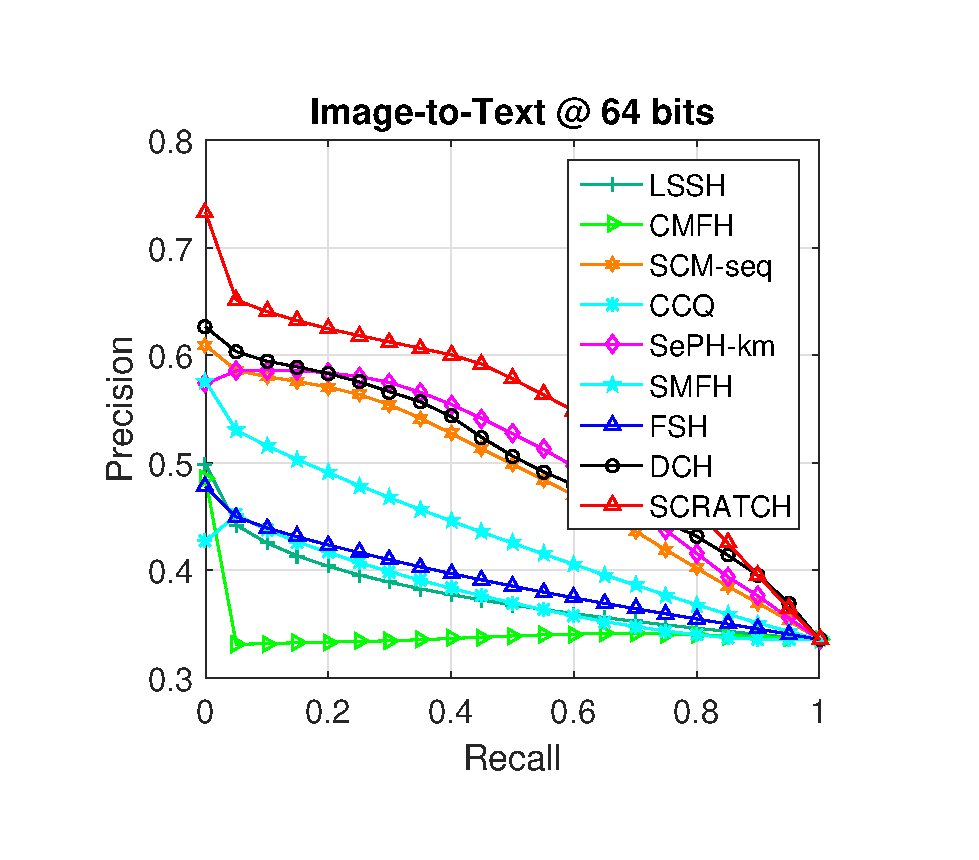
\includegraphics[width=8cm]{figures/NUS_WIDE_P_R/P_R_Image_Vs_Text_64}}
\end{minipage}
%\vspace{-6mm}
\begin{minipage}{0.5\linewidth}
\centering
\centerline{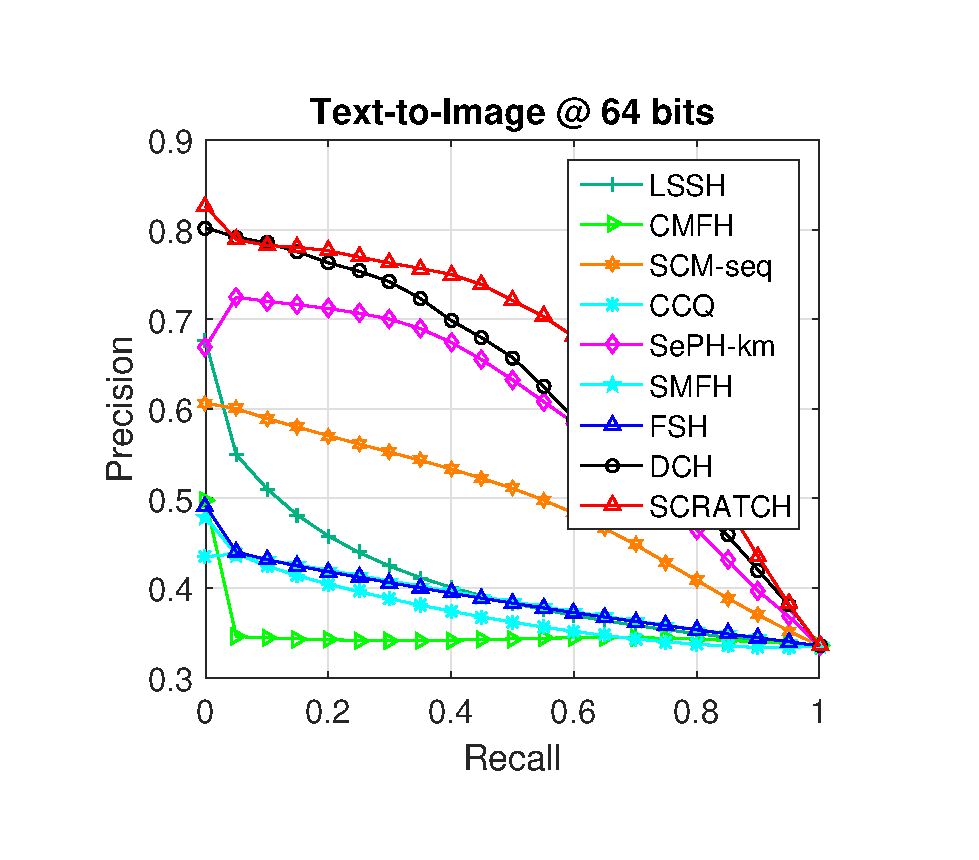
\includegraphics[width=8cm]{figures/NUS_WIDE_P_R/P_R_Text_Vs_Image_64}}
\end{minipage}
%\vspace{-4mm}
\caption{\bf NUS-WIDE ���ݼ�\ 64 λ��ϣ���\ Precision-Recall ����}
\label{curves-nus-3}\medskip
\end{figure*}


\begin{figure*}
\vspace{-12mm}
\begin{minipage}{0.5\linewidth}
\centering
\centerline{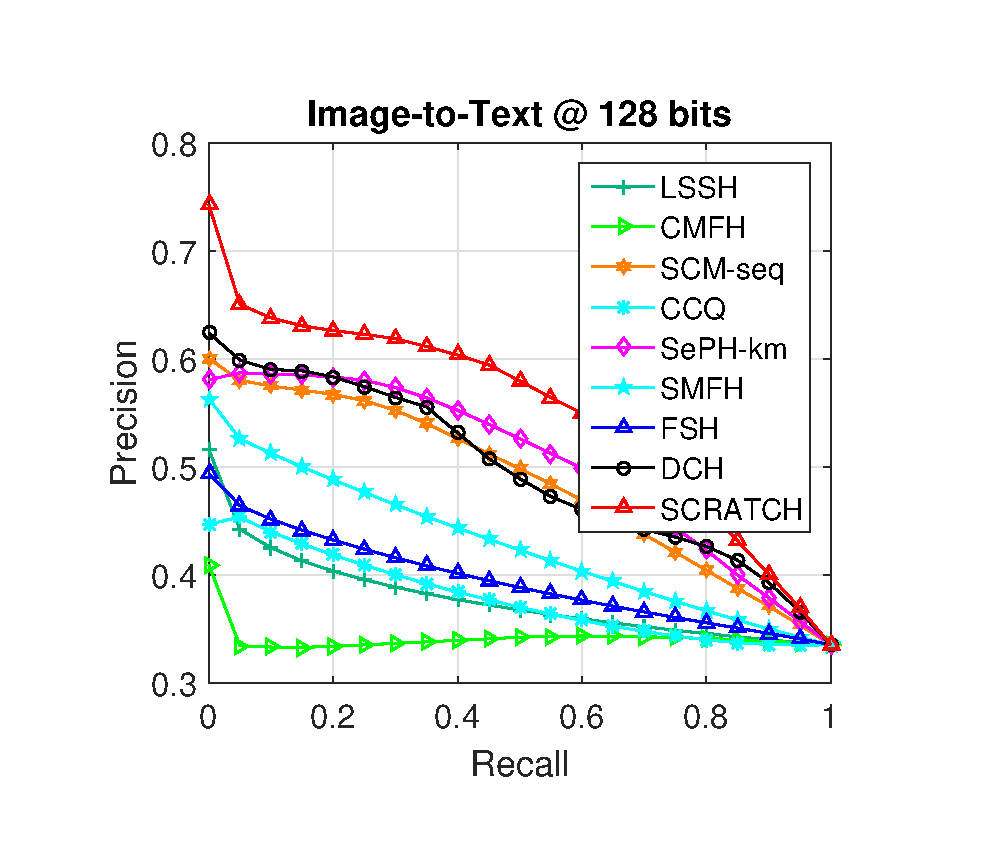
\includegraphics[width=8cm]{figures/NUS_WIDE_P_R/P_R_Image_Vs_Text_128}}
\end{minipage}
%\vspace{-6mm}
\begin{minipage}{0.5\linewidth}
\centering
\centerline{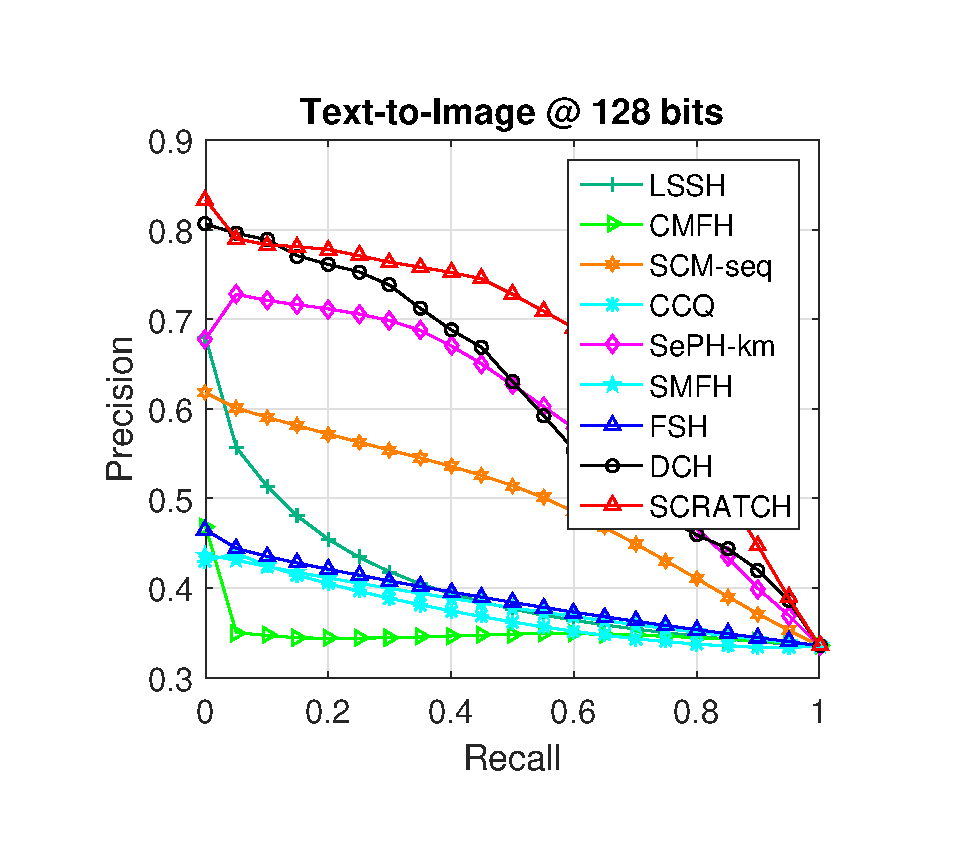
\includegraphics[width=8cm]{figures/NUS_WIDE_P_R/P_R_Text_Vs_Image_128}}
\end{minipage}
\caption{\bf NUS-WIDE ���ݼ�\ 128 λ��ϣ���\ Precision-Recall ����}
\label{curves-nus-4}\medskip
\end{figure*}


\begin{table}[tb]
%\setlength{\belowcaptionskip}{-0.3cm}
\small
\center
\begin{center}
\caption{\bf NUS-WIDE ���ݼ�����\ MAP �����ܶԱ�}
\label{mAP_nus}
%\vspace{-3mm}
\label{NUSWIDEmAP}
\begin{tabular}{cllllll}
  \toprule[1pt]
  Task & Method & 8 bits & 16 bits & 32 bits & 64 bits & 128 bits\\
  \hline
  \multirow{8}{*}{\tabincell{c}{Image\\to\\Text}}
  & {LSSH} & {0.3829} & {0.3885} & {0.3869} & {0.3911} & {0.3877}\\
  & {CMFH} & {0.3406} & {0.3437} & {0.3399} & {0.3409} & {0.3440}\\
  & {SCM-seq} & {0.5013} & {0.5120} & {0.5422} & {0.5488} & {0.5483}\\
  & {CCQ} & {0.3902} & {0.3959} & {0.3929} & {0.4010} & {0.3952}\\
  & {SePH-km} & {0.5256} & {0.5537} &{0.5627} & {0.5622} & {0.5698}\\
  & {SMFH} & {0.3711} & {0.4006} & {0.4461} & {0.4593} & {0.4594}\\
  & {FSH} & {0.3620} & {0.3732} & {0.3894} & {0.4014} & {0.4084}\\
  & {DCH} & {0.5840} & {0.5808} & {0.5907} & {0.5932} & {0.5843}\\
  & {SCRATCH} & {\bf{0.6038}} & {\bf{0.6207}} & {\bf{0.6338}} & {\bf{0.6459}} &{\bf{0.6496}}\\
  \hline
  \multirow{8}{*}{\tabincell{c}{Text\\to\\Image}}
  & {LSSH} & {0.4075} & {0.4202} & {0.3444} & {0.4231} & {0.4175}\\
  & {CMFH} & {0.3456} & {0.3498} & {0.3435} & {0.3486} & {0.3529}\\
  & {SCM-seq} & {0.4709} & {0.4836} & {0.5067} & {0.5141} & {0.5161}\\
  & {CCQ} & {0.3716} & {0.3740} & {0.3712} & {0.3734} & {0.3765}\\
  & {SePH-km} & {0.6102} & {0.6407} & {0.6515} & {0.6608} & {0.6651}\\
  & {SMFH} & {0.3631} & {0.3789} & {0.4046} & {0.4048} & {0.3997}\\
  & {FSH} & {0.3623} & {0.3717} & {0.3835} & {0.3973} & {0.4007}\\
  & {DCH} & {0.7106} & {0.7103} & {0.7098} & {0.7260} & {0.7223}\\
  & {SCRATCH} & {\bf{0.7210}} & {\bf{0.7392}} &{\bf{0.7549}} & {\bf{0.7680}} &{\bf{0.7755}}\\
  \toprule[1pt]
\end{tabular}
\end{center}\smallskip
\end{table}



\subsection{NUS-WIDE ���ݼ�ʵ����}
\esubsection{Results on NUS-WIDE}
\label{sec:nus-wide}

���з�����\ NUS-WIDE ���ݼ��ϵ�\ MAP ʵ�����ڱ�\ \ref{mAP_nus} �н������ܽᣬNUS-WIDE ���ݼ���\ 64 λ��\ 128 λ��ϣ���ϵ�\ top-N precision ��\ precision-recall ������ͼ\ \ref{curves-nus-1}��\ref{curves-nus-4} �л���������Щʵ�����У����ǿ��Եõ����½��ۣ���Щ������\ Wiki ��\ MIRFlickr-25K ���ݼ��ϵ�ʵ��������ƣ�
\begin{itemize}
\vspace{-3mm}
\item SCRATCH �ڸ��������µļ������ܶ�Ҫ���������������жԱȷ�������֤�����ڴ��ģ���ݼ��ϵ�ʵ���ԡ�
\vspace{-3mm}
\item ���Ź�ϣ��λ�����ӣ�SCRATCH �ļ������ܳ���������˵�������Ĺ�ϣ���ܹ���������Ϣ�������ϣ���У��Ӷ�ʵ�ּ������ܵĿ���������
\vspace{-3mm}
\item �����������\ Text-to-Image �����ϵļ�������ҪԶԶ����\ Image-to-Text ���������\ Wiki ��\ MIRFlickr-25K ���ݼ�һ�¡�
\vspace{-3mm}
\item �����мල��ģ̬��ϣ��������\ SCRATCH��DCH��������ҪԶԶ��Խ�������޼ල��������\ CMFH ��\ FSH����˵��������������Ϣ�����ڹ�ϣ��������Ա��֣��Ӷ���������������ܣ���һ��˵�������üල������Ϣ����Ч�ԡ�
\vspace{-3mm}
\item SCRATCH �ڹ�ϣ��λ���ܵͣ���\ 8 ��\ 16 λ����ʱ����Ȼȡ����Զ���������Աȷ����ļ������ܡ�
\vspace{-3mm}
\item SCRATCH ��\ $N$ �dz�С��ʱ��Ҫ�������Աȷ������ָ��ã�������\ Image-to-Text �ϣ�����˵��\ SCRATCH �� \ $N$ ��Сʱ�ܹ������������ѯ��������ص����ݿ���������Լ���������˵�Ƿdz���Ҫ�ġ�
\end{itemize}

�ܶ���֮��SCRATCH ���������û�׼���ݼ���ȡ���˼��߾������ļ������ܣ�˵����ͬʱ�����ʽ�ı�ǩ������Ϣ�ͻ���Эͬ����ֽ��ھ��������������Ϣ���Ը��õؽ������������Եı��֣��Ӷ�ʹ�����ɵĹ�ϣ���������ߡ���������������Эͬ����ֽ�Ŀ�ģ̬��������\ CMFH ��\ SMFH����ȣ�SCRATCH �������������ݼ���ʵ���˸��õļ������ܣ��Ӷ�֤���˱����������ʧ�������Ż�ģʽ����Ч�ԣ��������ڼ����ǩ��������ϢǶ������������ת�������ɢ�Ż���������\ SCRATCH ԶԶ��Խ����������Эͬ����ֽ�Ŀ�ģ̬��ϣ������


\subsection{���������Է���}
\esubsection{Parameter sensitivity analysis}

������ǰ����˵��������׼���ݼ��϶Բ��������Խ������꾡��ʵ�飬ͨ��ÿ�ι̶��������б�����ֻ��һ��������һ����Χ�ڽ��б仯���õ����Ӧ�ı仯���ߣ��Ӷ��ܹ���ֱ�۵ع۲쵽�������������ȡֵ�����У�������\ $\lambda_1$ ��\ $\lambda_2$ ����������ģ̬Эͬ����ֽ����Ȩ�أ��������ǵ�ʵ���з��֣��������������ı仯�����ս����Ӱ��Ƚ�С��������Ǿ����Ե�����������������Ϊ\ $\lambda_1$ = $\lambda_2$ = 0.5������֮�⣬����Ҳ�������������Ե�ʵ����˵�����������\ SCRATCH �����ں��ٵ�ѵ������������ﵽ����״̬���Ӷ�ʵ�ֿ��ٵ�ѵ���Ż������Գ�����\ $\mu$��$\alpha$��$\gamma$ ���б仯ʱ����Ӧ���������ݼ���\ 64 λ��ϣ�����������ģ̬����������ȡ�õ� MAP ������ͼ\ \ref{curves-param-1} ��\ \ref{curves-param-2} �и�����ͬʱ�������ݼ���Ŀ�꺯��ֵ���ڵ��������ı仯Ҳ��ͼ\ \ref{curves-param-2} �л���������\ ``I-T'' ��\ ``T-I'' �ֱ����\ Image-to-Text ��\ Text-to-Image ���񡣴�����ʵ���������ǿ��Եó����¹۲�ͽ��ۣ�


\begin{figure}
\setlength{\belowcaptionskip}{-0.5cm}
%\vspace{-6mm}
\begin{minipage}{0.5\linewidth}
\centering
\centerline{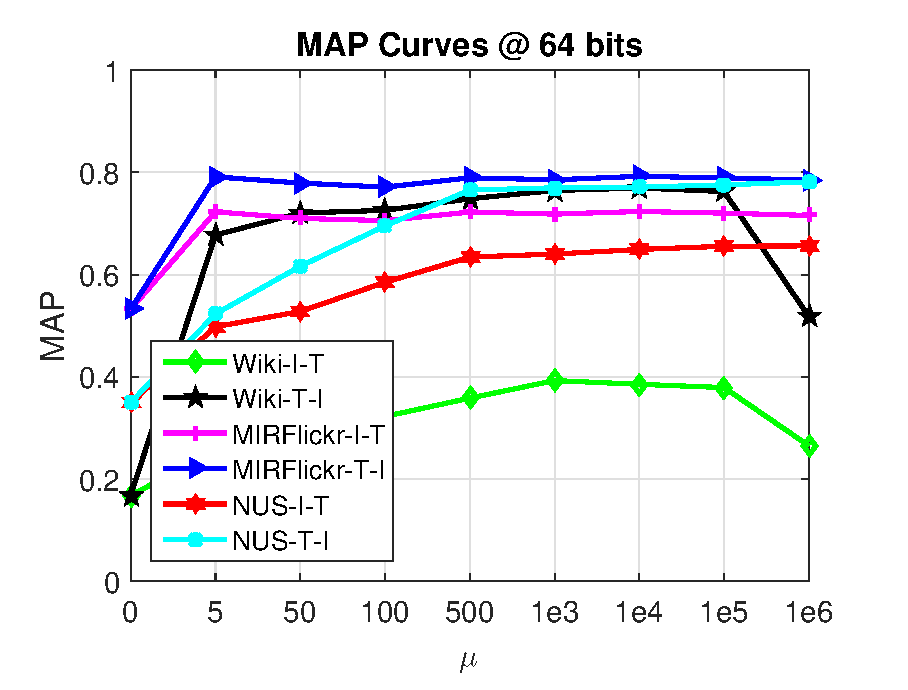
\includegraphics[width=8cm]{figures/Parameters/lambda}}
\end{minipage}
%\vspace{-6mm}
\begin{minipage}{0.5\linewidth}
\centering
\centerline{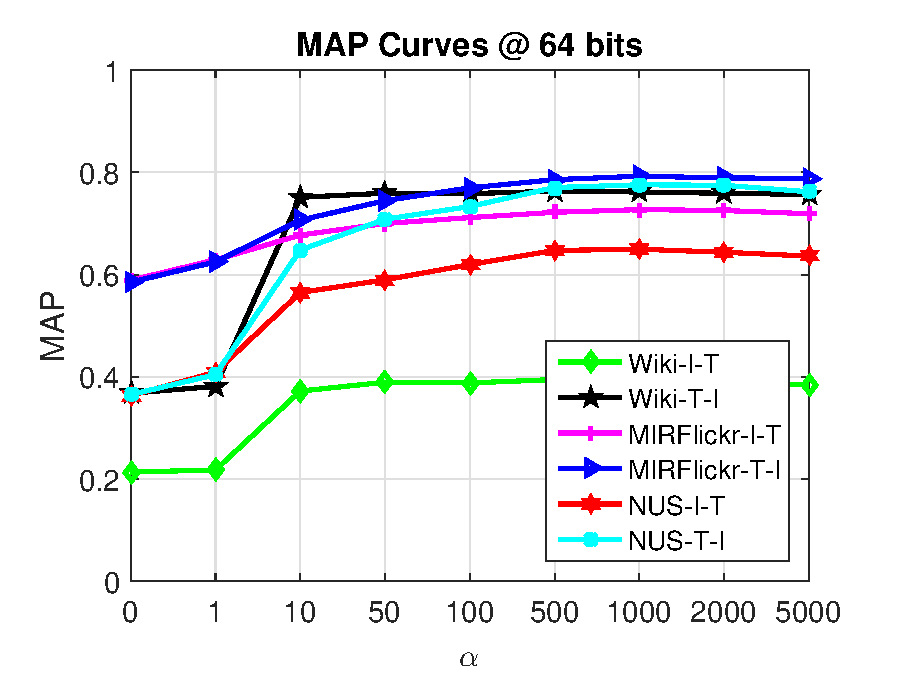
\includegraphics[width=8cm]{figures/Parameters/alpha}}
\end{minipage}
\caption{\bf ���ڳ�����\ $\mu$ ��\ $\alpha$ �IJ��������Է���}
\label{curves-param-1}
\end{figure}

\begin{figure}
\setlength{\belowcaptionskip}{-0.5cm}
\vspace{6mm}
\begin{minipage}{0.5\linewidth}
\centering
\centerline{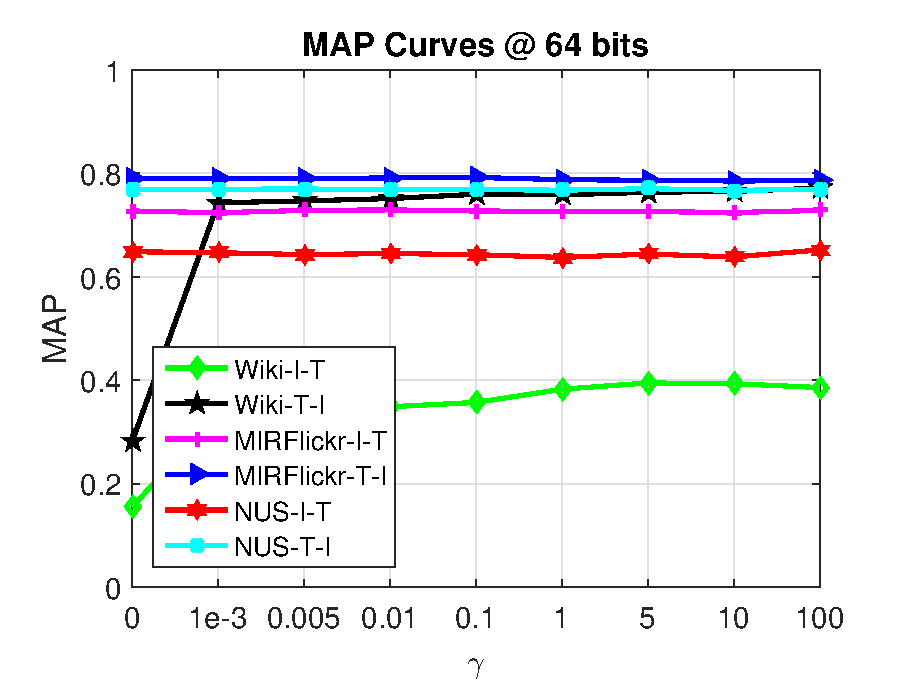
\includegraphics[width=8cm]{figures/Parameters/gamma}}
\end{minipage}
%\vspace{-6mm}
\begin{minipage}{0.5\linewidth}
\centering
\centerline{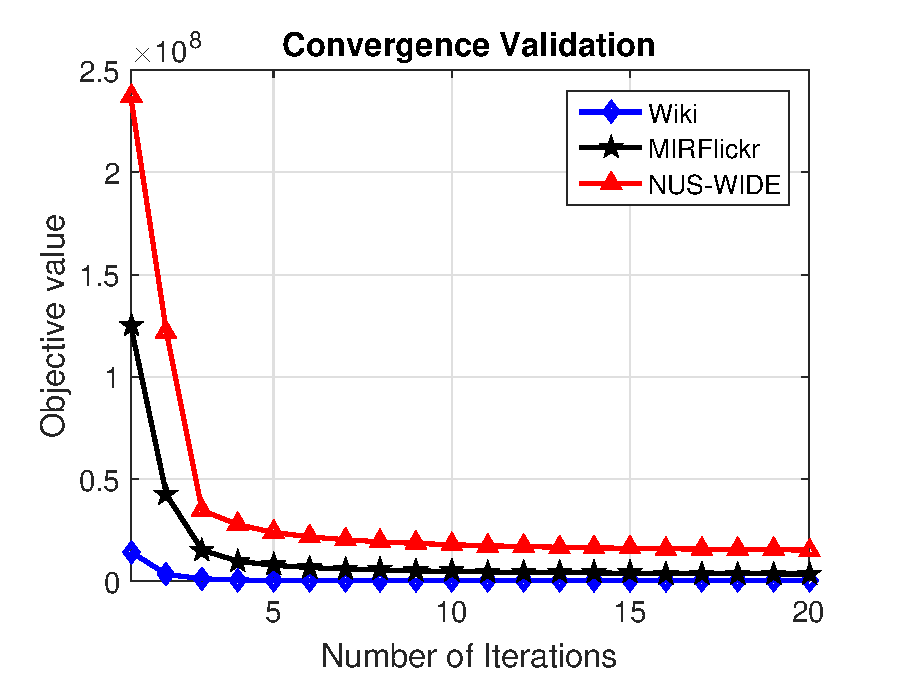
\includegraphics[width=8cm]{figures/Parameters/convergence}}
\end{minipage}
%\vspace{-3mm}
\caption{\bf ���ڳ�����\ $\gamma$ �͵��������IJ��������Է���}
\label{curves-param-2}
\end{figure}

\begin{itemize}
\vspace{-3mm}
\item \ $\mu$ ��\ $\alpha$ ȷʵ��Ӱ��\ SCRATCH �����ܣ�SCRATCH ��\ $\mu\approx1,000$ ��\ $\alpha\approx500$ ʱȡ�����Ž����
\vspace{-3mm}
\item ��\ $\mu$ ��\ $\alpha$ ��������ʱ��SCRATCH �����ܻ������½�������ζ�ŷ�����ӳ��ͱ�ǩ������Ƕ���ڱ��ķ���������������Ҫ�����á�
\vspace{-3mm}
\item \ $\gamma$ �������������Ȩ�أ���\ $\gamma\approx5$ ʱ\ SCRATCH ȡ�õļ�����������õġ�ֵ��һ����ǣ���\ $\gamma$ ������ʱ��SCRATCH ��\ Wiki ���ݼ��ϵļ������ܼ����½���Ȼ����\ MIRFlickr-25K ��\ NUS-WIDE ������Խϴ��ģ�����ݼ�����û�����������֣����ܵ�ԭ��Ϊ\ Wiki ���ݼ���һ��С���ݼ�������������С�ᵼ��\ SCRATCH �dz����׹���ϣ������������������������˷dz���Ҫ�ı������ϵ����ã�Ȼ��\ MIRFlickr-25K ��\ NUS-WIDE �������ݼ������ݹ�ģ����㹻�����\ SCRATCH �����������ݼ��ϲ����׷�����������󣬴Ӷ���������������ò������ԡ�
\vspace{-3mm}
\item SCRATCH �������������ݼ��Ͼ����ں��ٵĵ����������������״̬����һ��֤ʵ�˱���������Ż����Ե���Ч�Ժ�ʵ���ԡ�
\end{itemize}




\subsection{ʱ�����ķ���}
\esubsection{Time cost analysis}

Ϊ����֤���������\ SCRATCH ģ�͵���Ч�ԣ����ǽ�һ����\ MIRFlickr-25K ���ݼ��ϱȽ������з�����ѵ��ʱ�䣨����Ϊ��λ��ʱ������ϣ�볤��ȡ\ 8��16��32��64 ��\ 128 λ���Ӷ�����ֱ�۵ؿ�����ϣ��λ����ѵ��ʱ���Ӱ�죬���յ�ʵ�����ڱ�\ \ref{training_time} �н���չʾ����ʵ�������Կ��������Ź�ϣ��λ�������ӣ�SCRATCH ��ѵ��ʱ�䲢û���������ӣ�˵��\ SCRATCH ���Է���ĶԸ�ά���ݽ��п�ģ̬��ϣѧϰ������\ CMFH ���޼ල��ģ̬��ϣ������������жԱȷ�����ֻ��\ CMFH ��ѵ���ٶȿ���\ SCRATCH��Ȼ��������ǰ��С�������ģ����ǵ��ٶȺͼ������ȵ�ƽ�⣬CMFH�ļ�������ҪԶԶ����\ SCRATCH�������ۺ϶෽�濼�Ǽ����ٶȺͼ������ȵȣ�SCRATCH ���������ݼ��Ͼ��������ã�����\ SCRATCH ����Ч�ҷ������չ�����ģ���ݼ��ϡ�

\begin{table}[t]
\centering
\small
\caption{\bf MIRFlickr-25K ���ݼ��ϵ�ѵ��ʱ��Աȣ������ʱ��}
\label{training_time}
\resizebox{12cm}{!}{
\begin{tabular}{lrrrrrr}
\toprule[1pt]
%\hline
\multirow{1}{*}{Method}    & 8 bits & 16 bits & 32 bits & 64 bits & 128 bits \\
\hline
 {LSSH}  & {34.41} & {29.89} & {29.67} & {32.44} & {38.17} \\
 {CMFH} & {1.48} & {1.58} & {1.57} & {1.64} & {1.90}\\
 {SCM-seq} & {8.84} & {12.65} & {22.90} & {42.85} & {77.33}\\
 {CCQ} & {6.33} & {9.12} & {17.26} & {29.33} & {77.41}\\
 {SePH-km} & {3328.20} & {3411.26} & {3576.82} & {3805.26} & {4451.09}\\
 {SMFH} & {7.32} & {6.89} & {15.40} & {14.60} & {16.84}\\
 {FSH} & {109.59} & {108.25} & {107.52} & {109.73} & {115.55}\\
 {DCH} & {3.76} & {4.36} & {5.49} & {11.56} & {37.36}\\
 {SCRATCH} & {1.59} & {1.59} & {1.88} & {2.44} & {3.68}\\
\toprule[1pt]
\end{tabular}
}
\setlength{\belowcaptionskip}{-0.5cm}
\smallskip
\end{table}



\begin{table}[b]
\setlength{\abovecaptionskip}{-0.5cm}
\small
\center
\setlength{\abovecaptionskip}{0.1cm}
\begin{center}
\caption{\bf MIRFlickr-25K ���ݼ���\ SCRATCH ��\ DCMH ��\ MAP\ �Ա�}
\label{deep_extension}
\begin{tabular}{cllllll}
  \toprule[1pt]
  Task & Method & 8 bits & 16 bits & 32 bits & 64 bits & 128 bits\\
  \hline
  \multirow{2}{*}{\tabincell{c}{$I\rightarrow T$}}
  & {DCMH} & {0.7276} & {0.7247} & {0.7435} & {0.7484} & {0.7571}\\
  & {SCRATCH} & {\bf{0.7587}} & {\bf{0.7803}} &{\bf{0.7978}} & {\bf{0.8093}} &{\bf{0.8230}}\\
  \hline
  \multirow{2}{*}{\tabincell{c}{$T\rightarrow I$}}
  & {DCMH} & {0.7453} & {0.7580} & {0.7692} & {0.7758} & {0.7819}\\
  & {SCRATCH} & {\bf{0.7532}} & {\bf{0.7797}} &{\bf{0.7913}} & {\bf{0.7979}} & {\bf{0.8160}}\\
  \toprule[1pt]
\end{tabular}
\end{center}
\smallskip
\end{table}


\subsection{����ȹ�ϣ�����Ա�}
\esubsection{Comparison with Deep Hashing}

Ϊ��˵�������������ʧ�������Ż���������Ч�ԣ����ǽ�һ����\ MIRFlickr-25K ���ݼ�����һ����ǰ���ܽϺõ���ȿ�ģ̬��ϣ��DCMH��\cite{jiang2017dcmh}������ʵ��Աȡ���ѭ\ DCMH ��ʵ�����ã��������Ƚ�����\ DCMH ��ʹ�õ�\ CNN-F\cite{ken14cnnf} ������ȡ��ͼ��ģ̬�����������Ȼ���ڵõ������ͼ��������ԭʼ���ı�������ʹ��\ SCRATCH ���п�ģ̬��ϣ���������յ�\ MAP ʵ�����ڱ�\ \ref{deep_extension} �н������ܽᣬ�ӽ���п��Եó����¹۲죺
\begin{itemize}
\vspace{-3mm}
\item SCRATCH ��������ģ̬���������ϵ����ܾ�������\ DCMH��
\vspace{-3mm}
\item ���Ź�ϣ��λ�����ӣ�SCRATCH �ļ������ܳ���������˵�������Ĺ�ϣ���ܹ���������Ϣ�������ϣ���У��Ӷ�ʵ�ּ������ܵĿ���������
\vspace{-3mm}
\item SCRATCH ��\ Image-to-Text �����ϵ����Ź�ϣ��λ���ı仯���������ܾ��������\ DCMH��
\vspace{-3mm}
\item SCRATCH ����������ϵ�\ Image-to-Text ��������ҪԶԶ�������˹���ȡ�����ϵ����ܣ���ʹ�����ͼ��������\ SCRATCH �ڹ�ϣ��λ���ܵͣ���\ 8 ��\ 16 λ��ʱ\ Image-to-Text ����ļ��������Ѿ�������ʹ���˹�����\ SCRATCH �ڸ�λ��ϣ�루128 λ�������ܣ�˵����Ⱦ�����������ȡ����ͼ����������Խ�ԡ�
\end{itemize}



%
%\subsection{������չ}
%\esubsection{Extension to classification}
%
%
%
%\begin{table*}[t]\scriptsize
%\caption{CLASSIFICATION performance comparison of various models on MIRFlickr-25000 and NUS-WIDE.}\label{table_classification}
%\centering
%\begin{tabular}{cccccccccccccc}
%\toprule[1pt]
%\multirow{3}{*}{Task} & \multirow{3}{*}{Method} & \multicolumn{6}{c}{MIRFlickr} & \multicolumn{6}{c}{NUS-WIDE}\\
%\cmidrule(lr){3-8} \cmidrule(lr){9-14}
%&& \multicolumn{3}{c}{MacroF1} & \multicolumn{3}{c}{Accuracy} & \multicolumn{3}{c}{MacroF1} & \multicolumn{3}{c}{Accuracy} \\
%
%\cmidrule(lr){3-5}  \cmidrule(lr){6-8} \cmidrule(lr){9-11} \cmidrule(lr){12-14} & &16 bits & 32 bits & 64 bits & 16 bits & 32 bits & 64bits & 16 bits & 32 bits & 64 bits & 16 bits & 32 bits & 64bits\\ \hline
%\multirow{8}{*}{\tabincell{c}{ Image }}
%
% {}&CVH & 0.0627 & 0.0486 & 0.0463 & 0.1428 & 0.1229 & 0.1184  & 0.1129 & 0.0858 & 0.0651 & 0.1648 & 0.1394 & 0.1288 \\
% {}&IMH & 0.0521 & 0.0586  &0.0590& 0.0998& 0.1207 & 0.1250 & 0.0806 & 0.0890  &0.1001& 0.1021& 0.1060 & 0.1233 \\
% {}&SCM-seq  & 0.0834 & 0.0820& 0.0900 & 0.1580 & 0.1642& 0.1814 & 0.2062 & 0.1985& 0.2159& 0.3051 & 0.2798& 0.3066\\
% {}&LSSH & 0.0750 & 0.0722 & 0.1115 & 0.1144 & 0.1106 & 0.1653 & 0.1908 & 0.2030 & 0.2227 & 0.2283 & 0.2362 & 0.2781 \\
% {}&CMFH & 0.0824 & 0.0243 & 0.0265 & 0.1488 & 0.0831 & 0.0830 & 0.0505 & 0.0492 & 0.0484 & 0.1075 & 0.1098 & 0.1093 \\
% {}&FSH & 0.0801 & 0.0874 & 0.0910 & 0.1415 & 0.1410 & 0.1448 & 0.1623 & 0.2026 & 0.2320 & 0.2324 & 0.2915 & 0.3132 \\
% {}&SePH-km & 0.1664 & 0.1926 & 0.1997 & 0.2719 & 0.2704 & 0.2732 & 0.2718 & 0.2781 & 0.2561 & 0.3520 & 0.3470 & 0.3414\\
% {}&SRDMH & \textbf {0.2240} & {\textbf{0.2554}} & {\textbf{0.2784}} & {\textbf{0.2793}} & {\textbf{0.2710}} & {\textbf{0.2749}} & \textbf {0.2919} & {\textbf{0.3036}} & {\textbf{0.4251}}& {\textbf{0.3702}} & {\textbf{0.3896}} & {\textbf{0.4207}} \\
%\hline
%\multirow{8}{*}{\tabincell{c}{ Text }}
% {}&CVH & 0.0716 & 0.0673 & 0.0758 &0.1565 & 0.1482 & 0.1513 & 0.1497 & 0.1580 & 0.1652 &0.2222 & 0.2170 & 0.2296 \\
% {}&IMH & 0.0458 & 0.0688 & 0.1218 &0.0893 & 0.1156 & 0.1637 & 0.0732& 0.1424 & 0.2158 &0.0815& 0.1581 & 0.2477 \\
% {}&SCM-seq & 0.1682 & 0.2464 & 0.3125 & 0.3187 & 0.3597 & 0.3830 & 0.3770& 0.4336 & 0.4765 & {\textbf {0.4933}} & 0.5028 & 0.5357\\
% {}&LSSH & 0.1343 & 0.2033 & 0.2503  & 0.1495 & 0.1966 & 0.2622 & 0.2794& 0.3060 & 0.3422  & 0.3326 & 0.3492 & 0.3958\\
% {}&CMFH & 0.1068 & 0.0312 & 0.0314& 0.1838 & 0.0806 & 0.0806 & 0.0519 & 0.0504 & 0.0502 & 0.1114 & 0.1115 & 0.1087\\
% {}&FSH & 0.0738 & 0.0882 & 0.0992  & 0.1270 & 0.1454 & 0.1637 & 0.1650& 0.2294 & 0.2747 & 0.2242 & 0.3269 & 0.3677\\
% {}&SePH-km & 0.2135 & 0.2802 & 0.2818& 0.3353 & 0.3807 & 0.3860 & 0.4021 & 0.4225 & 0.3957 & 0.4923 & 0.5026 & 0.5048 \\
% {}&SRDMH & {\textbf {0.3018}} & {\textbf{0.3658}} & {\textbf{0.4085}}& {\textbf {0.3375}} & {\textbf{0.3824}} & {\textbf{0.3867}} & \textbf {0.4022} & {\textbf{0.4545}} & {\textbf{0.5608}}& {\textbf{0.4933}} & {\textbf{0.5069}} & {\textbf{0.5387}} \\\hline
%\toprule[1pt]
%\end{tabular}
%\end{table*}

\section{������}
\esection{Summary}

��������ͨ��\ MAP �Աȡ�top-N precision ��\ precision-recall �����Լ�ѵ��ʱ��Աȵ�ʵ�����������֤��\ SCRATCH ����Ч�ԣ�ͬʱ����ȿ�ģ̬��ϣ�����Աȣ�����ʹ����Ⱦ����������\ SCRATCH ����һ���˵��˵����ģ�ͣ�����ͬʱѵ�������\ SCRATCH ģ�ͣ�������ȡ��ģ��ѵ���Ƿֿ��ģ���������Ȼȡ���˳�Խ��ǰ�Ƚ�����ȿ�ģ̬��ϣ������DCMH���ļ������ܣ����һ��˵����\ SCRATCH ���õ���ʧ�������Ż����Ե��Ƚ��Ժ���Ч�ԡ�


\chapter{\quad\quad �ܽ���չ��}
\label{chap6}
\echapter{Conclusions and Future Works}

\section{�ܽ�}
\esection{Conclusions}

��������������Ϣ�����ķ��ٷ�չ�Լ��ƶ��豸�������罻��վ�����У���ý�����ݳ��ֱ�ըʽ��������������ģ̬����������������ά�ȸ��Լ�Ҫ����Ӧ�ٶȿ���ص㣬��ϣ��������洢С��������ŵ㣬Ϊ����Щ��嫵Ķ�ģ̬���ݿ��з��㡢���١�׼ȷ�ز�ѯ���������û�����Ļ����Ȥ��ģ̬��Ϣ�ṩ�˽������������𽥳�Ϊ���ģ��ģ̬���ݼ��������о����ȵ㡣

Ŀǰ���кܶ��ģ̬��ϣ�����������ȡ���˲����Ŀ�ģ̬����Ч�����������м������������ܵ�������ڣ�1) һЩ��������ɢ���������ɳڻ����������ɵĹ�ϣ���нϴ��������ʹ�����չ�ϣ��ļ���Ч���½���2) Ҳ��һЩ����ֱ�ӽ�����ɢ�Ż�������������ѵ��ʱ��Ϊ���ۣ������Ż�����ʱ�������ӣ�3) �ڼල��Ϣ��ѡ���ϣ��еķ���ѡ��ʹ��\ $n\times n$ �������Ծ�����������Ա��֣�����ᵼ����ѵ����ʱ�临�Ӷ�������$O(n^2)$����������������չ�����ģ���ݼ����Ѷȡ�

�ۺϿ�����������֮�󣬱������һ���µ��мල��ϣ�����������ھ���ֽ�Ŀ���չ��ɢ��ϣ�����Ϊ\ SCRATCH���÷�����ԭʼ�����˻�����о���ֽ⣬����ϱ�ǩ��Ϣ������Ƕ��������һ�������ӿռ䣬�Ӷ������ܵı���ģ̬���ģ̬�ڵ����������ԣ�ͬʱ��ͨ��ʹ�ñ�ǩ������������Ծ��󣬸÷�����ѵ�����Ӷ�ʼ�������ݼ���ģ����Ϊ���Թ�ϵ���ɷ������չ�����ģ��ģ̬���ݼ��ϣ�Ϊ�˽����ɢ�Ż����⣬����������ת��������С��ѵ�������е���������ʹ�õ����Ż��ķ�ʽ����һ����С�������������������û�׼���ݼ��ϵ�ʵ�������SCRATCH �ɴﵽ��ǰ��ϣ�������Ƚ�ˮƽ���������������ɽ�һ���������ģ̬�������ܣ�ͬʱ������ѵ���ٶȿ졢����չ�����ģ���ݼ����ŵ㣬չ�ֳ����ߵ���Ч�Ժ�ʵ���ԡ�



\section{չ��}
\esection{Future Works}

ֵ��һ����ǣ�SCRATCH ������һ������ȿ�ģ̬����ģ�ͣ���Ϊ������Ƹ�ģ�͵ij���������ʧ�������Ż����ԵĴ����ԡ���С�ڣ�3.3.6����ʾ������\ SCRATCH ����һ���˵��˵����ģ�ͣ�����ͬʱѵ�������\ SCRATCH ģ�ͣ�������ȡ��ģ��ѵ���Ƿֿ��ģ�������ȡ�ó�Խ��ǰ�Ƚ�����ȿ�ģ̬��ϣ������DCMH���ļ������ܣ�˵��\ SCRATCH ���õ���ʧ�������Ż���������ȷ����Ч�ģ����ǵ��˵��˵ľ���������͹�ϣѧϰѵ������ʹ�����ߵĽ�ϸ��ӽ��ܣ�ͬʱҲ��õ����õؼ���Ч����������Ǽƻ������е���ʧ����Ƕ�뵽����������У�����ģ̬��ӳ�亯��Ҳ������������������棬�Ӷ�����һ���˵��˵���ȿ�ģ̬��ϣģ�͡�

����֮�⣬�������ǵķ���ʹ������ʽ�������ǩ����ѵ����ͬʱʹ���˾���ֽ����ھ��ģ̬����������������Ϣ��ȥ��������Ϣ����˱���\ SCRATCH ģ��ѧ���Ĺ�ϣ����𵥶��������ǩ��˵��ͬʱ�������ʽ����ʽ�ķḻ������Ϣ��������õ��Ĺ�ϣ�����ڷ��࣬����Ԥ������Ч��Ӧ�ú���ʹ��ԭʼ�������з��࣬��Ϊԭʼ���ݵ�����������Ϣδ���ھ�ͬʱ�����ܰ������������������յķ�����Ӱ��ܴ�ʹ�ù�ϣ����з������һ���ô��ǣ��൱�ڶ�ԭʼ���ݽ����˽�ά����������������С�����ݵĴ洢�ռ�ͷ�����ѵ�������ģ����ͬʱҲ�������˷����������ܡ�


%\cleardoublepage

%\chapter{\quad\quad ���ٿ���չ�ල��ϣ����}
\label{chap4}
\echapter{Fast Scalable Supervised Hashing}


��������һ�������һ����Ч�ļල��ϣ�������÷���������һ���м��������ֱ��ʹ��������ƽ����С��������ɶ������Ծ��󡣾�������м���Ĵ�СԶС��������ɶ������Ծ��󣬵������С������������������صģ������ݺܴ��ʱ���Ի��кܸߵ����ġ����⣬��һ�µķ�������������ȱ�ݡ���һ��SSDHʹ���˰�λ�Ż��IJ�����ѧϰ��ϣ�룬�����ѵ��ʱ��������Թ���������ڹ�ϣ��ѧϰ�Ĺ����У�SSDH������ԭʼ���ݵ�������Ϣ������ʹ�üල��Ϣָ����ϣ������ɡ�

�����ڱ��������һ����Ϊ���ٿ���չ�ල��ϣ���·�������Ӣ����ΪFast Scalable Supervised Hashing����дΪFSSH�����÷���ͬ��������һ���м������м���Ĵ�СԶС��������ɶ������Ծ��������������޹أ�ֻ���������������ά���йء���ˣ��÷������Ը��õؼ�С�ռ����ļ��Ż����Ӷȡ����⣬���Dz�����һ���Ż�����λ��ϣ�����ɢ�Ż��㷨������׼ȷ����Ч����ɹ�ϣ��ĸ��¡������ڹ�ϣ��ѧϰ�Ĺ����У�ͬʱ�����˼ල��Ϣ�����ݵ�ԭʼ������Ϣ��������֤�˹�ϣ���׼ȷ�ԡ�ͨ���ڳ������ݼ��ϵ�ʵ�飬���ǿ��Է��ָ÷����������еļල��ϣ����������֮�⣬ʵ�鼰���۷�������ʾ�����µķ�������ǰһ������ķ�����







\section{����}
\esection{Introduction}

���кܶ๤�����������ල��ϣѧϰ��Ч������޼ල��ϣѧϰ�úܶ�\cite{da2017amvh,kang2016column,wang2016deep}�������ڱ������о��ı���һ�ּල��ϣģ�͡�

�����з����У��ල��ϣģ�͵ķ�ʽ�ж��֣������б�ʹ������Ŀ�꺯�����£�
\begin{equation}\label{fssheq1}
\begin{split}
   &  \min_\textbf{B}\parallel r \textbf{S}  -\textbf{B} \textbf{B}^\top   \parallel_F^2,\\
   & s.t. \ \ \ \textbf{B}\in\{-1,1\}^{n\times r},
\end{split}
\end{equation}
���У�$\parallel \cdot \parallel_F$��Frobenius����������$r$�ǹ�ϣ���λ����$\textbf{S}\in\{-1,1\}^{n\times n}$ ������֮��ɶԵ����������Ծ���$\textbf{S}_{ij}=1$��ζ�������������������������Ƶģ���֮$\textbf{S}_{ij}=-1$����$\textbf{B}$�ǰ���$n$ ��������ϣ��ľ���

��ʽ\ref{fssheq1}��һ����ɢ�Ż����⣬�����������ѽ�ġ�һЩ���й���\cite{lin2013general,liu2012supervised} �������������ʱ�򣬲�ȡ�ķ�ʽ���£��Ȱѹ�ϣ�����ɢԼ�������ɳڳɷ���ɢ���Ӷ��������һ������������õ�һ���⣬�����������������ɢ�Ĺ�ϣ�롣���ڵ�һЩ����\cite{lin2014fast,kang2016column,luo2018scalable}������ֱ����ɢ����⹫ʽ\ref{fssheq1}������ʵ���б�������Щ��������Щ���ɳ������ķ������кܶ��Ч�����������в�����ǣ���Щ���������õ��ǰ�λ����ϣ��IJ��ԣ�Ҳ����˵������������ǰһλ��ϣ����ܼ��������һλ�Ĺ�ϣ�롣������ϣ���λ���ܶ��ʱ����Щ���������ٶ���������ӡ����⣬��Ϊ��ʽ\ref{fssheq1}�еijɶԵ������Ծ���Ĵ�С��$n \times n$ �ģ��������ֱ��ʹ��$\textbf{S}$�ᵼ��$O(n^2)$ ��ʱ�临�ӶȺͿռ临�Ӷȡ�Ϊ�˱�����ô��Ŀ�����һЩ������ѵ����ʱ����Ϊ�ز�������������ȥѵ�������ִ�����ʽ�������Ϣ����ʧ���Ӷ�Ӱ�����յĽ��������һЩ�����������в����IJ��ԣ�����LFH\cite{zhang2014supervised}��COSDISH\cite{kang2016column}�����ǿ����������е�ѵ�����ݣ�����Ч����ǰһ�ַ����úܶࡣ����������\cite{zhang2014supervised} ��ʵ�����У��������ܷ��֣��в��������һ����Ч���½���SSDH\cite{luo2018scalable}���������ŰѳɶԵ������Ծ���$\textbf{S}$Ƕ�뵽һ����ά�ռ�ľ�����ȥ���������Ĵ�С��$n \times c$ �ģ����У�$c$�������������$c$ԶС��$n$�������������С����ѵ��������$n$ �йأ��ҵ�$n$ �ܴ��ʱ���临�Ӷ��Ի�ܸߡ����ٲ��ù�ʽ\ref{fssheq1} ��������ʧ�����Ĺ�ϣ����\cite{zhang2014supervised,kang2016column,luo2018scalable}���������ɹ�ϣ���ʱ��������������Ϣ�������������ݵ�������

Ϊ�˽���������з����ľ��ޣ���Ҫ����������ȥ��⹫ʽ\ref{fssheq1}����һ��������Ҫ��Ч���������е�ѵ�����ݣ������ʹ�ò�����������ɵ���Ϣ��ʧ�������������Ҫ�����ɢ���Ż��㷨����������㷨Ӧ����ʹ�ð�λ�Ż����ԡ��������ڼල��ϣ������ɵ�ʱ������Ӧ�������������Ϣ������Ҫ�������ݱ�����������Ϣ��

�����ڱ��������һ����ӱ�ļල��ϣģ�ͣ�����Ϊ���ٿ���չ�ල��ϣ������Ӣ����ΪFast Scalable Supervised Hashing�����¼��ΪFSSH��



\section{��ط�������}
\esection{Related Work}

\subsection{������ϣ}
\esubsection{Two-Step Hashing}

���������ǵķ����ж�����壬���в���һ����ϣ���Եı��壬Ҳ�в���������ϣ������Ƶı��塣���������ֱ��壬���Ƿ����ĺ��������ڵ�һ������ʧ����������Լ���Ӧ���Ż��㷨��

����������ϣ����ؽ��ܣ���ο��½�\ref{chap-tsh}��

\subsection{����չ�ල��ɢ��ϣ}
\esubsection{Scalable Supervised Discrete Hashing}

�뱾�·�������ص�һ�����й�ϣ�����ǿ���չ�ල��ɢ��ϣ������Scalable Supervised Discrete Hashing����дΪSSDH��������SSDH ����ϸ�㷨��ο���\ref{chap3}�¡�

����SSDH����Ƴ�����FSSH�ij����в����ص�������С$n \times n$��������ɶ������Ծ�����ɵľ޴����ģ��Լ���ɢ���Ż���ϣ�롣���������ڴ�Ҫǿ��SSDH ���������㣺1��SSDH��$n \times n$��������ɶ������Ծ���Ƕ�뵽һ���м����У���������м���Ĵ�С�����������йأ����������ܴ��ʱ�򣬸�������Ҫ�ܴ�Ŀռ䡣2��SSDH���õ��ǰ�λ�Ż���ϣ��IJ��ԣ������IJ���ͨ���ܺ�ʱ��3���ڹ�ϣ�����ɵĹ����У�SSDH��ʹ���˼ල�������Ϣ�������ܳ�ֿ��ǵ����ݱ�����

�������е�FSSH���������SSDH���������ƣ�1����Ȼͬ���ǰ�$n \times n$��������ɶ������Ծ���Ƕ�뵽һ���м����У�FSSH �õ����м���Ĵ�С�����������޹صģ������м����SSDH���м���ҪС�Ķࡣ2��FSSH������һ���Ż���ϣ������λ�IJ��ԣ��ò�����ʱ��������Ҫ����SSDH �İ�λ�Ż����ԡ�3��FSSH������ѧϰ��ϣ���ʱ�򣬼ȿ����˼ල�������Ϣ���ֿ��Գ������ý�����ݱ�����




\section{���ٿ���չ�ල��ϣ����}
\esection{Fast Scalable Supervised Hashing}

\subsection{���ź���������}
\esubsection{Notations and Problem Definition}

����$n$������$\textbf{X}=[\textbf{x}_1, \textbf{x}_2, \cdots, \textbf{x}_n] \in\mathbb{R}^{n\times d}$����ϣģ�͵�Ŀ�����ڱ���ԭ�ռ�������Ե�ǰ����ѧ����Щ������$r$λ��ϣ�룻���У�$\textbf{b}_i$������$\textbf{x}_i$ ��Ӧ�Ĺ�ϣ�룬$d$��������ά������ʧһ���ԣ����Ǽ�����ڱ�ǩ������������������ı�ǩ$\textbf{L}=[\textbf{l}_1, \textbf{l}_2, \cdots, \textbf{l}_n]\in\{0,1\}^{n\times c}$�����У�$c$������������$\textbf{l}_{ik}$��$\textbf{l}_i$�ĵ�$k$λԪ�أ�����������������$k$�Ļ�����$\textbf{l}_{ik}=1$����֮$\textbf{l}_{ik}=0$�� ���⣬$\textbf{S}$ ������֮��ɶԵ����������Ծ������У�$\textbf{S}_{ij}=1$��ζ������$i$������$j$�������������Ƶģ�������߲���������${S}_{ij}=-1$�� �����е���ط���һ�£����Ǽ������$\sum^n_{i=1} \textbf{x}_i=0$��

��Ϊ�˻����Ը��õIJ�׽ԭʼ�����еķ����Խṹ�����������ڹ�ϣ�о�����õ��˹㷺��Ӧ��\cite{da2017amvh,gui2018fast,huang2016class,liu2012supervised,shen2015supervised}�� ����������ʹ��RBF�˺���������صģ����������ȡ$m$������Ϊê�㣬${\textbf{o}_1, \textbf{o}_2, \cdots, \textbf{o}_m}$��ͨ���˺���$\phi(\textbf{x})=[exp(\frac{-\parallel \textbf{x}-\textbf{o}_1 \parallel_2^{2}}{2\sigma^{2}}),\cdots ,exp(\frac{-\parallel \textbf{x}-\textbf{o}_m \parallel_2^{2}}{2\sigma^{2}})]^\top$���԰�ÿһ����������ӳ���$m$ ά�ĺ������������$\sigma$��ͨ����ѵ������֮���ŷʽ����ȡ��ֵ�õ��ġ�




\subsection{Ŀ�꺯��}
\esubsection{Objective Function}

\subsubsection{������ӳ��}
\esubsubsection{Kernel Features Mapping}

��ϣ�����������ǰ����ݴ�ԭʼ����ת���ɹ�ϣ�룬���ǿ��԰ѹ�ϣ����д��������ʽ��
\begin{equation}\label{fssheq2}
 F(\textbf{X})=sgn(\phi(\textbf{X})\textbf{W})=\textbf{B}
\end{equation}	
���У�$\textbf{W}\in \mathbb{R}^{m\times r}$��һ����ԭ����ת�䵽$r$άʵֵ�ռ��ͶӰ����$sgn(\cdot)$�Ƿ��ź���������Ϊ����$x\geq 0$ ʱ$sgn(x)=1$����$x<0$ʱ$sgn(x)=-1$�������������ǿ���ͨ�����µ�ʽ��������������ӳ���������
\begin{equation}\label{fssheq3}
\begin{split}
   &  \min_{\textbf{W}}\parallel \textbf{B}  -\phi(\textbf{X})\textbf{W}   \parallel_F^2,\\
   & s.t. \ \ \ \textbf{B}\in\{-1,1\}^{n\times r}.
\end{split}
\end{equation}	
���⣬���й���\cite{gordo2014asymmetric,da2017amvh}���������ѹ�ʽ\ref{fssheq1}�еĹ�ϣ�뻻Ϊʵֵ����Ϣ�����Ը��õؽ��Ƴɶ������Ծ�����ˣ�Ϊ����ѧϰ��ϣ��Ĺ������ܸ��õ�������������Ϣ��������ʵֵ��$\phi(\textbf{X})\textbf{W}$ ���滻����һ��$\textbf{B}$��
\begin{equation}\label{fssheq4}
\begin{split}
  &  \min_{\textbf{B},\textbf{W}}\parallel  \textbf{S}  -\big(\phi(\textbf{X})\textbf{W}\big) \textbf{B}^\top   \parallel_F^2,\\
   & s.t. \ \ \ \textbf{B}\in\{-1,1\}^{n\times r}.
\end{split}
\end{equation}
�ѹ�ʽ\ref{fssheq3}�͹�ʽ\ref{fssheq4}����һ�����ǵõ���
\begin{equation}\label{fssheq5}
\begin{split}
   &  \min_{\textbf{B},\textbf{W}} \parallel  \textbf{S}  -\big(\phi(\textbf{X})\textbf{W}\big) \textbf{B}^\top   \parallel_F^2+\mu \parallel \textbf{B}  -\phi(\textbf{X})\textbf{W}   \parallel_F^2\\
   & s.t. \ \ \ \textbf{B}\in\{-1,1\}^{n\times r},
\end{split}
\end{equation}	
����$\mu$�Dz�����

\subsubsection{������Ƕ��}
\esubsubsection{Label Matrix Embedding}

��Ȼ�ɶ������Ծ���$\textbf{S}$��������$\textbf{L}$������������Ϣ�����ҳɶ������Ծ�������ɺ��߼���õ��������������Ժ��кܶ����õ���Ϣ��������������������������Ƕ�Ӧ������ǩΪ$\textbf{l}_1=[1,0,0]$��$\textbf{l}_2=[1,1,1]$ ��$\textbf{l}_3=[1,1,1]$���ڳɶ������Ծ���$\textbf{S}$ ����${S}_{13}={S}_{23}=1$��������1������2֮�����Ƴ̶�С������1������3����ʵȴ�޷�����Ӧ����ˣ�����ϣ���ڹ�ϣ��ѧϰ�����л��ܹ����ǵ�������$\textbf{L}$�����Ǽ��裺ͨ������һ���任����$\textbf{G}\in \mathbb{R}^{c\times r}$����������Ա�ͶӰ����ϣ��ռ䲢��Ϲ�ϣ�롣�õ�����ʽ�ӣ�
\begin{equation}\label{fssheq6}
\begin{split}
   &  \min_{\textbf{B},\textbf{G}}\parallel \textbf{B}  -\textbf{LG}   \parallel_F^2,\\
   & s.t. \ \ \ \textbf{B}\in\{-1,1\}^{n\times r}.
\end{split}
\end{equation}

\subsubsection{����Ŀ�꺯��}
\esubsubsection{Overall Objective Function}


����ʽ\ref{fssheq5}�͹�ʽ\ref{fssheq6}��ϣ���������һ��$\textbf{B}$���������Ŀ�꺯�����£�
\begin{equation}\label{fssheq7}
\begin{split}
   &  \min_{\textbf{B},\textbf{G},\textbf{W}}\parallel \textbf{S}-\big(\phi(\textbf{X})\textbf{W}\big)(\textbf{LG})^\top\parallel_F^2\\
   & +\mu\parallel \textbf{B}-\textbf{LG}\parallel_F^2 +\theta \parallel \textbf{B}-(\phi(\textbf{X})\textbf{W})\parallel_F^2,\\
   & s.t. \ \ \ \textbf{B}\in\{-1,1\}^{n\times r},
\end{split}
\end{equation}	
����$\mu$��$\theta$���Dz�����

��ʽ\ref{fssheq7}����������������Ϣ���ɶ������Ծ������������ʹ��ѧ���Ĺ�ϣ����Ը��õı���ԭ�е����������ԡ�ֵ��ע����ǣ���Ȼ��ʽ�а����˾���$\textbf{S}$���Ⲣ����ζ�����ᱻֱ��ʹ�á����ǽ����������½�����ϸ���������ͨ������һ����Ԥ�ȼ�����м�������ﵽ���Ż��б���ֱ��ʹ��$n\times n$�ijɶ������Ծ���



\subsection{�Ż��㷨}
\esubsection{Optimization}

Ϊ���Ż���ʽ\ref{fssheq7}�����������һ�������Ż��㷨������㷨��ÿһ�������������������衣����������ֱ��Ϊ$\textbf{W}$ ���裬$\textbf{G}$ �����$\textbf{B}$���裻��ÿ�������У����������������̶���ֻ���µ�ǰ������


\subsubsection{$\textbf{W}$����}
\esubsubsection{$\textbf{W}$ Step}

����������У����ǹ̶�����$\textbf{G}$��$\textbf{B}$����ʽ\ref{fssheq7}�ɼ�Ϊ��
\begin{equation}\label{fssheq8}
  \min_{\textbf{W}}\parallel \textbf{S}-\big(\phi(\textbf{X})\textbf{W}\big)(\textbf{LG})^\top\parallel_F^2 +\theta \parallel \textbf{B}-\phi(\textbf{X})\textbf{W}\parallel_F^2.
\end{equation}
ͨ���Դ�ʽ����$\textbf{W}$�󵼲�ȡ0�����ǿ��Եõ���ʽ�ӵ�һ���ս⣺
\begin{equation}\label{fssheq9}
\begin{split}
& \ \ \ \textbf{W}=\big(\phi(\textbf{X})^\top \phi(\textbf{X})\big)^{-1}\\
&\big(\phi(\textbf{X})^\top \textbf{SLG} + \theta \phi(\textbf{X})^\top \textbf{B}\big)(\textbf{G}^\top \textbf{L}^\top \textbf{LG} +\theta \textbf{I}_{r\times r})^{-1},
\end{split}
\end{equation}
��һ����������$\textbf{A}=\phi(\textbf{X})^\top \textbf{SL}$��$\textbf{C}=\phi(\textbf{X})^\top \phi(\textbf{X})$ ��$\textbf{D}=\textbf{L}^\top \textbf{L}$������ʽ���Ը�дΪ��
\begin{equation}\label{fssheq10}
\begin{split}
& \ \ \ \textbf{W} =\textbf{C}^{-1}\big(\textbf{AG} + \theta \phi(\textbf{X})^\top \textbf{B}\big)(\textbf{G}^\top \textbf{D} \textbf{G} +\theta \textbf{I}_{r\times r})^{-1},
\end{split}
\end{equation}
���ǿ���ע�⵽��$\textbf{C}$��$\textbf{D}$��Ϊ������������Ż�֮ǰ����ã�������ÿ�ε��������¼��㡣

���������������һ���м���$\textbf{A}\in \mathbb{R}^{m\times c}$����Ȼ������Ҳ��һ��������ҿ������Ż�ǰ����ã����Ż�������ֱ��ʹ�á����Ҹ�������˳ɶ������Ծ������Ż�ʱֱ��ʹ��$\textbf{A}$ ���Ա���ֱ��ʹ��$\textbf{S}$������������$O(n^2)$�ĸ��Ӷȡ�


\subsubsection{$\textbf{G}$����}
\esubsubsection{$\textbf{G}$ Step}

ÿ�ε����еĵڶ���Ϊ������$\textbf{G}$�IJ��衣�̶�����$\textbf{W}$��$\textbf{B}$����ʽ\ref{fssheq7}��дΪ����$\textbf{G}$��Ŀ�꺯����
\begin{equation}\label{fssheq11}
  \min_{\textbf{G}} \parallel \textbf{S}-\big(\phi(\textbf{X})\textbf{W}\big)(\textbf{LG})^\top\parallel_F^2 +\mu\parallel \textbf{B}-\textbf{LG}\parallel_F^2.
\end{equation}
ͬ���ģ���ʽ����$\textbf{G}$����ȡ�㣬���ǿ��Ի��һ���⣺
\begin{equation}\label{fssheq12}
\begin{split}
&\ \ \ \textbf{G}=(\textbf{L}^\top \textbf{L})^{-1}\\
& \big(\mu \textbf{L}^\top \textbf{B}+ \textbf{L}^\top \textbf{S}^\top \phi(\textbf{X})\textbf{W}\big)\big(\textbf{W}^\top \phi(\textbf{X})^\top \phi(\textbf{X})\textbf{W} +\mu \textbf{I}_{r\times r}\big)^{-1}. \\
\end{split}
\end{equation}
���ǿ��Է��֣�������$\textbf{A}$��$\textbf{C}$��$\textbf{D}$�����ڸ�ʽ�������õ���
\begin{equation}\label{fssheq13}
\begin{split}
&\ \ \ \textbf{G} =\textbf{D}^{-1}(\mu \textbf{L}^\top \textbf{B}+ \textbf{A}^\top \textbf{W})(\textbf{W}^\top \textbf{CW} +\mu \textbf{I}_{r\times r})^{-1}.\\
\end{split}
\end{equation}

\subsubsection{$\textbf{B}$����}
\esubsubsection{$\textbf{B}$ Step}

�����������$\textbf{B}$����ʱ���ǹ̶�ס�����������õ����µ����⣺
\begin{equation}\label{fssheq14}
\begin{split}
   &  \min_{\textbf{B}} \ \mu\parallel \textbf{B}-\textbf{LG}\parallel_F^2 +\theta \parallel \textbf{B}-\phi(\textbf{X})\textbf{W}\parallel_F^2,\\
   & s.t. \ \ \ \textbf{B}\in\{-1,1\}^{n\times r}.
\end{split}
\end{equation}
Ȼ�����ǿ��԰���ʽչ���ɼ�����ʽ�����£�
\begin{equation}\label{fssheq15}
\begin{split}
   &  \min_{\textbf{B}} \ \mu Tr \Big( (\textbf{B}-\textbf{LG})^\top (\textbf{B}-\textbf{LG})\Big)\\
   & \quad \quad +\theta Tr\Big(\big(\textbf{B}-\phi(\textbf{X})\textbf{W}\big)^\top\big(\textbf{B}-\phi(\textbf{X})\textbf{W}\big)\Big),\\
   & = (\mu +\theta )\parallel \textbf{B}\parallel^2_F -2\mu Tr(\textbf{B}^\top \textbf{LG})\\
   & +\mu \parallel \textbf{LG}\parallel^2_F -2\theta Tr\big(\textbf{B}^\top \phi(\textbf{X})\textbf{W}\big) +\theta\parallel \phi(\textbf{X})\textbf{W}\parallel^2_F,\\
   & s.t. \ \ \ \textbf{B}\in\{-1,1\}^{n\times r},
\end{split}
\end{equation}
���У�$Tr(\cdot)$�Ǿ���ļ�����Ϊ$\parallel \textbf{B}\parallel^2_F$��$\parallel \textbf{LG}\parallel^2_F$ ��$\parallel \phi(\textbf{X})\textbf{W} \parallel^2_F$��Ϊ����������������ǵõ����µ��Ż�Ŀ�꣺
\begin{equation}\label{fssheq16}
\begin{split}
   &  \min_{\textbf{B}} -Tr \Big(\textbf{B}^\top \big(\mu \textbf{LG}+\theta \phi(\textbf{X})\textbf{W} \big) \Big),\\
   & s.t. \ \ \ \textbf{B}\in\{-1,1\}^{n\times r}.
\end{split}
\end{equation}
�����ʽ�ӵıս�Ϊ��
\begin{equation}\label{fssheq17}
\textbf{B}= sgn\big(\mu \textbf{LG}+\theta \phi(\textbf{X})\textbf{W}\big), \\
\end{equation}

�ӹ�ʽ\ref{fssheq18}�����ǿ���ֱ�۵Ŀ�������ÿ�ֵ�����ֻ��Ҫһ��������λ�Ĺ�ϣ�����Ա����¡��������Ż���ʽ��Ȱ�λ�Ż���ϣ��IJ��Խ�Լʱ�����ġ�




\subsection{��������չ}
\esubsection{Out-of-Sample Extension}

�����Ѿ������ѵ�����ݵĹ�ϣ�룬����ѵ���������������������Ҫʹ�ù�ϣ����Ϊ�����������Ӧ�Ĺ�ϣ�롣����ƹ�ϣ������ʱ������������ѡ�񣬴Ӷ�����������㷨�����ֱ��壬�ֱ���һ����ϣ���Ա��壨��ΪFSSH\_os����������ϣ���Ա��壨FSSH\_ts����

����������ֱ���֮ǰ�����Ǽ���$\textbf{X}_{query}$��$\textbf{B}_{query}$�ֱ��Dz�ѯ���ݵ�ԭʼ����������Ҫѧ���Ĺ�ϣ�롣


\subsubsection{һ����ϣ����FSSH��FSSH\_os}
\esubsubsection{One-Step FSSH: FSSH\_os}

һ����ϣ����ֱ��ʹ������ϣ��ʱͬʱѧ����$\textbf{W}$������������ϣ��������û�ж����ѧϰ���̡�����ζ�ţ���ϣ���ѧϰ�͹�ϣ������ѧϰ��ͬ�����еģ�ֻ��Ҫһ�����ɣ��ʳ�Ϊһ����ϣ���Ա��塣
��ˣ����ڲ�ѯ���ݣ����ǿ��������µ�ʽ�Ӽ������ǵĹ�ϣ�룺
\begin{equation}\label{fssheq18}
\textbf{B}_{query}=sgn(\phi(\textbf{X}_{query})\textbf{W}).
\end{equation}


\subsubsection{������ϣ����FSSH��FSSH\_ts}
\esubsubsection{Two-Step FSSH: FSSH\_ts}

������ϣ���岻ʹ��$\textbf{W}$��������Ҫ����ȥѧϰ��ϣͶӰ����FSSH\_ts����������ϣ�IJ��ԣ��Ҹ���ǰ�ĵĽ��ܣ���ʱ������Ҫ������������$\phi(\textbf{X})$�͹�ϣ�����$\textbf{B}$��ѧϰ�����Ʒ����������κ���Ч�ķ����������ﶼ���Ա�ʹ�á��ڴˣ����ǵ�Ч�����⣬����ѡ�����Իع�������FSSH\_ts �Ĺ�ϣ������

��ʱ���������������任Ϊ��ϣ���ͶӰ����$\textbf{P}$����ͨ���Ż������ƽ�����õ���
\begin{equation}\label{fssheq19}
\parallel \textbf{B}-\phi(\textbf{X})\textbf{P} \parallel^2_F + \lambda_e \parallel  \textbf{P}\parallel^2_F,
\end{equation}
���У�$\lambda_e$�Dz�����$\parallel  \textbf{P}\parallel^2_F$����������յĽ�Ϊ��
\begin{equation}\label{fssheq20}
\textbf{P}=\big(\phi(\textbf{X})^\top \phi(\textbf{X})+ \lambda_e \textbf{I}\big)^{-1}\phi(\textbf{X})^\top \textbf{B}.
\end{equation}

��ˣ����ڲ�ѯ���ݣ����ǿ��������µ�ʽ�Ӽ������ǵĹ�ϣ�룺
\begin{equation}
\textbf{B}_{query}=sgn(\phi(\textbf{X}_{query})\textbf{P}).
\end{equation}






\section{ʵ�������ͽ������}
\esection{Experiments}

�ڱ����У������������������ݼ�ʹ�����ǵķ�������ý���������ͬʱ��Ϊ�˿͹۵Ŀ������ǵķ������������з�����ѡΪ��׼�����������ǵķ������Ƚϡ�

\subsection{���ݼ�}
\esubsection{Datasets}

\textbf{CIFAR-10���ݼ�}\cite{krizhevsky2009learning}����һ��������$60000$��ͼƬ�Ĺ������ݼ�������һ������$10$�����ĵ���ǩ���ݼ�������ζ�ţ�ÿһ��ͼƬ������ֻ����һ�����ÿһ������������$6000$��ͼƬ���ڱ�ʵ���У����Ƕ�ÿһ��ͼƬ����ȡ$512$ά��GIST�����������á����⣬���������ȡ$1000$��ͼƬ������ʵ��IJ��Լ�������ʣ�µ�$59000$��ͼƬ��Ϊʵ��ѵ�������������ʱ���������ͼƬ��Ӧ�����һ�£���������ͼƬ���ƣ��������ͼƬ��Ӧ�����ͬ������Ϊ������ͼƬ�Dz����Ƶġ�

\textbf{MNIST���ݼ�}\cite{lecun1998gradient}:������$70000$��ͼƬ���ǻ���ѧϰ������õ����ݼ�֮һ����ЩͼƬ�����������֡�0�������֡�9������д�壬��ÿ��ͼƬֻ����һ����д���֡���ˣ�������ݼ���һ������ǩ���ݼ����ҹ���$10$������ڱ�ʵ���У�ÿ��ͼƬ����784 ά��������������ʾ�����������ȡ$1000$ ��ͼƬ������ʵ��IJ��Լ�������ʣ�µ�69000��ͼƬ��Ϊʵ��ѵ�������������ʱ���������ͼƬ��Ӧ�����һ�£���������ͼƬ���ƣ��������ͼƬ��Ӧ�����ͬ������Ϊ������ͼƬ�Dz����Ƶġ�

\textbf{NUS-WIDE���ݼ�}\cite{chua2009nus}�������¼��¹�����ѧ���о���Ա���������ݼ�������ͼƬ���Ǵ�ͼƬ��վFlickr ���ռ��ģ�������$269648$ ��ͼƬ��������ݼ��ʼ����$81$ �����Ϊ���뱾��������й�������һ�µ�ʵ��������������SDH������ɸѡ�����г��ִ�������$21$��������Ӧ��$195834$��ͼƬ������һ�����ǩ���ݼ���Ҳ����˵��ÿ��ͼƬ���Զ�Ӧ�ڶ����ǩ��ʵ���У�ÿ��ͼƬ������ʾΪһ��$500$ά�Ĵʴ��������ڹ������Լ���ʱ�����Ǵ�ÿ����������������$100$�ţ�����$2100$��ͼƬ��Ϊ���յIJ��Լ�������ʣ�µ�ͼƬ��Ϊ���ǵ�ѵ����������ʱ���������ͼƬ������һ��������ǩ����ô������ͼƬ�ͱ���Ϊ�����Ƶģ���֮���������ͼƬû�й�����ǩ����ô���Ǿ��Dz����Ƶġ�


\subsection{�Աȷ�����ʵ��ϸ��}
\esubsection{Baselines and Implementation Details}

����ѡ��6�����з���������ʵ��Ƚϡ���Щ��������Supervised Hashing with Kernels��KSH��\cite{liu2012supervised}��Supervised Discrete Hashing ��SDH��\cite{shen2015supervised}��Fast Supervised Discrete Hashing ��FSDH��\cite{gui2018fast}�� Two-Step Hashing��TSH��\cite{lin2013general}��Supervised Hashing with Latent Factor Models ��LFH��\cite{zhang2014supervised}��Column Sampling Based Discrete Supervised Hashing ��COSDISH��\cite{kang2016column}�����У�ǰ���ַ�������һ����ϣ����������������������ϣ������

FSDH�Ĵ��������������������е�����ʵ�֣���FSDH֮��ķ����Ĵ����ʹ��ԭ�����ṩ�Ĵ��롣���з����IJ����������������еĽ������á����⣬��ΪKSH ��TSH�ļ��㸴�ӶȽϸߣ����������е��������\cite{shen2015supervised,kang2016column}������ֻ�������ѵ��������������$2000$��ͼ��ѵ��������ģ�͡�
�������ǵķ�����������������£���FSSH\_os��$\mu=10000$��$\theta=100$����FSSH\_ts��$\mu=10000$��$\theta=0.01$��$\lambda_e=1$��$m=1000$��

����ʵ������ж�Σ�����ÿ�ζ��������ѵ���Ͳ��Լ������յ�ʵ�������ڶ��ʵ��Ļ�����ȡƽ��ֵ�õ���

ʵ�黷����һ̨���������û����������Ϣ���£�Intel(R) XEON(R) CPU E5-2650@2.30GHz��128GB�ڴ档



\subsection{����ָ��}
\esubsection{Evaluation Metrics}

������������ع��������Dz������ֱ��㷺ʹ�õ����۱�׼����ֵƽ�����ȣ�mean average precision MAP����ǰN׼ȷ�����ߣ�top-N precision curves����׼ȷ��-�ٻ������ߣ�precision recall curves�����������ֱ�׼��˵����ֵԽ�����������Ч��Խ�á�

�������������۱�׼�Ľ��ܣ���ο��½�\ref{chap-EvaMet}��


\subsection{����Ƚ�}
\esubsection{Comparison Results}

\subsubsection{��ֵƽ�����Ⱥ�ʱ��Ƚ�}
\esubsubsection{MAP and Time}

%\begin{table*}[t]\tiny\center
%\caption{�������ݼ��ϵ�MAP�����λ����ͬ�������õ�ʵ�������Ӵ���ʾ��}\label{chap4map}
%\begin{tabular}{c||cccc||cccc||cccc}\hline
% \multirow{2}{*}{Method} &\multicolumn{4}{c||}{CIFAR-10}&\multicolumn{4}{c||}{MNIST}&\multicolumn{4}{c}{NUS-WIDE}\\
%\cline{2-13}
%&16 bits&32λ&64λ&96λ&16λ&32λ&64λ&96λ&16λ&32λ&64λ&96λ\\\hline
%{KSH}&{0.2626}&{0.2897}&{0.3108}&{0.3185}&{0.8017}&{0.8233}&{0.8390}&{0.8400}&{0.3703}&{0.3728}&{0.3785}&{0.3786}\\
%{SDH}&{0.3525}&{0.3788}&{0.3986}&{0.4135}&{0.8718}&{0.8873}&{0.8958}&{0.8972}&{0.4113}&{0.4114}&{0.4135}&{0.4211}\\
%{FSDH}&{0.3284}&{0.3661}&{0.3986}&{0.4110}&{0.8562}&{0.8804}&{0.8907}&{0.8962}&{0.4052}&{0.4115}&{0.4155}&{0.4166}\\\hline
%{TSH}&{0.3202}&{0.3551}&{0.3711}&{0.3843}&{0.9007}&{0.9215}&{0.9281}&{0.9323}&{0.4424}&{0.4479}&{0.4555}&{0.4545}\\
%{LFH}&{0.3803}&{0.5061}&{0.6133}&{0.6288}&{0.5564}&{0.7577}&{0.8593}&{0.8575}&{0.5767}&{0.5974}&{0.6042}&{0.6124}\\
%{COSDISH}&{0.5737}&{0.6109}&{0.6310}&{0.6368}&{0.8551}&{0.8754}&{0.8818}&{0.8888}&{0.5719}&{0.5913}&{0.5916}&{0.6027}\\\hline
%{FSSH\_os}&{0.3896}&{0.5592}&{0.6497}&{0.6760}&{0.9023}&{0.9480}&{0.9360}&{0.9311}&{0.4813}&{0.5255}&{0.5867}&{0.6029} \\
%{FSSH\_ts}&\textbf{0.6350}&\textbf{0.6829}&\textbf{0.7071}&\textbf{0.7108}&\textbf{0.9443}&\textbf{0.9649}
%&\textbf{0.9713}&\textbf{0.9721}&\textbf{0.5846}&\textbf{0.6060}&\textbf{0.6105}&\textbf{0.6225} \\\hline
%\end{tabular}\end{table*}

\begin{table}[t]\center%\small
\caption{CIFAR-10���ݼ��ϵ�MAP�����λ����ͬ�������õ�ʵ�������Ӵ���ʾ��}\label{chap4mapcifar}
\begin{tabular}{ccccc}\hline
 {Method}& 16λ  & 32λ  & 64λ  & 96λ  \\\hline
{KSH}&{0.2626}&{0.2897}&{0.3108}&{0.3185}\\
{SDH}&{0.3525}&{0.3788}&{0.3986}&{0.4135}\\
{FSDH}&{0.3284}&{0.3661}&{0.3986}&{0.4110}\\
{TSH}&{0.3202}&{0.3551}&{0.3711}&{0.3843}\\
{LFH}&{0.3803}&{0.5061}&{0.6133}&{0.6288}\\
{COSDISH}&{0.5737}&{0.6109}&{0.6310}&{0.6368}\\\hline
{FSSH\_os}&{0.3896}&{0.5592}&{0.6497}&{0.6760} \\
{FSSH\_ts}&\textbf{0.6350}&\textbf{0.6829}&\textbf{0.7071}&\textbf{0.7108} \\\hline
\end{tabular}\end{table}

\begin{table}[t]\center%\small
\caption{MNIST���ݼ��ϵ�MAP�����λ����ͬ�������õ�ʵ�������Ӵ���ʾ��}\label{chap4mapmnist}
\begin{tabular}{ccccc}\hline
 {Method}& 16λ  & 32λ  & 64λ  & 96λ  \\\hline
{KSH}&{0.8017}&{0.8233}&{0.8390}&{0.8400}\\
{SDH}&{0.8718}&{0.8873}&{0.8958}&{0.8972}\\
{FSDH}&{0.8562}&{0.8804}&{0.8907}&{0.8962}\\
{TSH}&{0.9007}&{0.9215}&{0.9281}&{0.9323}\\
{LFH}&{0.5564}&{0.7577}&{0.8593}&{0.8575}\\
{COSDISH}&{0.8551}&{0.8754}&{0.8818}&{0.8888}\\\hline
{FSSH\_os}&{0.9023}&{0.9480}&{0.9360}&{0.9311} \\
{FSSH\_ts}&\textbf{0.9443}&\textbf{0.9649}
&\textbf{0.9713}&\textbf{0.9721} \\\hline
\end{tabular}\end{table}

\begin{table}[t]\center%\small
\caption{NUS-WIDE���ݼ��ϵ�MAP�����λ����ͬ�������õ�ʵ�������Ӵ���ʾ��}\label{chap4mapnus}
\begin{tabular}{ccccc}\hline
 {Method}& 16λ  & 32λ  & 64λ  & 96λ  \\\hline
{KSH}&{0.3703}&{0.3728}&{0.3785}&{0.3786}\\
{SDH}&{0.4113}&{0.4114}&{0.4135}&{0.4211}\\
{FSDH}&{0.4052}&{0.4115}&{0.4155}&{0.4166}\\\
{TSH}&{0.4424}&{0.4479}&{0.4555}&{0.4545}\\
{LFH}&{0.5767}&{0.5974}&{0.6042}&{0.6124}\\
{COSDISH}&{0.5719}&{0.5913}&{0.5916}&{0.6027}\\\hline
{FSSH\_os}&{0.4813}&{0.5255}&{0.5867}&{0.6029} \\
{FSSH\_ts}&\textbf{0.5846}&\textbf{0.6060}&\textbf{0.6105}&\textbf{0.6225} \\\hline
\end{tabular}\end{table}

\begin{figure}[t]
\begin{minipage}{0.49\linewidth}\centering
\centerline{\includegraphics[width=7.5cm]{Images/chap4/C32PN.eps}}\centerline{\footnotesize(a) CIFAR-10 32 λ}\medskip
\end{minipage}
\begin{minipage}{0.49\linewidth}\centering
\centerline{\includegraphics[width=7.5cm]{Images/chap4/C96PN.eps}}\centerline{\footnotesize(b) CIFAR-10 96 λ}\medskip
\end{minipage}\\
\begin{minipage}{0.49\linewidth}\centering
\centerline{\includegraphics[width=7.5cm]{Images/chap4/M32PN.eps}}\centerline{\footnotesize(c) MNIST 32 λ}\medskip
\end{minipage}
\begin{minipage}{0.49\linewidth}\centering
\centerline{\includegraphics[width=7.5cm]{Images/chap4/M96PN.eps}}\centerline{\footnotesize(d) MNIST 96 λ}\medskip
\end{minipage}\\
\begin{minipage}{0.49\linewidth}\centering
\centerline{\includegraphics[width=7.5cm]{Images/chap4/N32PN.eps}}\centerline{\footnotesize(e) NUS-WIDE 32 λ}\medskip
\end{minipage}
\begin{minipage}{0.49\linewidth}\centering
\centerline{\includegraphics[width=7.5cm]{Images/chap4/N96PN.eps}}\centerline{\footnotesize(f) NUS-WIDE 96 λ}\medskip
\end{minipage}\\
\caption{���з������������ݼ��ϵ�ǰN׼ȷ�����ߣ����й�ϣ��λ��Ϊ32��96λ��}\medskip\label{chap4PN}\end{figure}



��\ref{chap4mapcifar}����\ref{chap4mapmnist}�ͱ�\ref{chap4mapnus}�ֱ��г�����CIFAR-10��MNIST��NUS-WIDE���ݼ��ϵ�ʵ����������Щ�������������µķ��֣�
\begin{itemize}
\item ���ǵķ���FSSH\_os��Ч���ϱ����е�һ����ϣ�Աȷ�����Ҫ�á����嵽��ֵ�У���CIFAR-10���ݼ��ϣ�FSSH\_os ����õ�һ����ϣ��Ч���ϻ����$10.5\%$��16λ����$47.6\%$��32 λ����$63.0\%$��64 λ����$63.5\%$��96λ������������MNIST ���ݼ��ϣ�FSSH\_os �������õ�һ����ϣ��Ч��������$3.53\%$��16 λ����$6.84\%$��32λ����$4.49\%$��64 λ����$3.78\%$��96 λ������NUS-WIDE���ݼ��ϣ���Ӧ������Ϊ$17.0\%$��16 λ����$27.7\%$ ��32 λ����$41.9\%$��64 λ����$43.2\%$��96 λ����
\item ���Ƿ�����������ϣ�汾FSSH\_ts�������Ҫ�������е�������ϣ�Աȷ�����
\item FSSH\_ts���������ݼ�������λ������£���ȡ������ѵ�ʵ��Ч�������������棬������ϣ��������һ����ϣ������
\item FSSH\_os��ʵ������SDH��FSDH�Ľ������˺ܶ࣬��һ������ԭ���ǣ�FSSH\_os��ѧϰ�����������˳ɶԵ������Ծ����Լ���ǩ���󣬶�SDH�� FSDH ����ʹ���˱�ǩ����ͬʱ���Աȷ���LFH��COSDISHҲ�����˳ɶԵ������Ծ��󣬲������ǵ�ʵ��Ч��Ҳ����SDH ��FSDH����Щ�������ij�̶ֳ�����ʾ������ڱ�ǩ���󣬳ɶԵ������Ծ�������ܸ��õؼල��ϣ������ɡ�
\item FSSH\_ts��Ч����LFH��COSDISH��Ч�����ã����ܵ�ԭ������������һ��LFH�� COSDISHΪ�˱������ĸ��Ӷȣ���ѧϰ�����о�ʹ�����в����������������ܻᵼ����Ϣ��ʧ������ʹЧ���½��������FSSH\_ts ��LFH��COSDISH �࿼���˱�ǩ������ѵ���п��Ǹ���ļල��Ϣ���п��ܻ�ѧϰ�����Ӿ�׼�Ĺ�ϣ�롣
\end{itemize}
�ܶ���֮�����ǵķ�����Ч���ϱ����з������ã�������ʾ��������Ƶ���ʧ�������Ż���������֮��Ч�ġ�




\subsubsection{ǰN׼ȷ�����߱Ƚ�}
\esubsubsection{Top-N Precision Curves}







ͼ\ref{chap4PN}������ǰN׼ȷ�����ߣ���ͼ�����ǿ��������·��֣�
\begin{itemize}
\item ��CIFAR-10���ݼ��ϡ����ǵķ���FSSH\_os�����е�һ����ϣ��׼ȷ��ͬʱ��������ϣ�汾FSSH\_ts �����߸������е�������ϣ�Աȷ��������ҿ��Է��ָ����������������������������ߡ�
\item ��MNIST���ݼ��ϡ�FSSH\_os��Ȼ�����е�һ����ϣ��׼ȷ����FSSH\_tsҲ�����е�������ϣ�Աȷ�����׼ȷ��
\item ��NUS-WIDE���ݼ��ϡ�ʵ��������ǰ�������ݼ��ϵĽ��һ�£����ǵ�һ����ϣ��������ϣ�������ȶ�Ӧ��һ����ϣ��������ϣ�Աȷ������á�
\item ���������ݼ�����������£�FSSH\_tsһֱ������õĽ����
\end{itemize}

\begin{figure}[t]
\begin{minipage}{0.49\linewidth}\centering
\centerline{\includegraphics[width=7.5cm]{Images/chap4/C32PR.eps}}\centerline{\footnotesize(a) CIFAR-10 32 λ}\medskip
\end{minipage}
\begin{minipage}{0.49\linewidth}\centering
\centerline{\includegraphics[width=7.5cm]{Images/chap4/C96PR.eps}}\centerline{\footnotesize(b) CIFAR-10 96 λ}\medskip
\end{minipage}\\
\begin{minipage}{0.49\linewidth}\centering
\centerline{\includegraphics[width=7.5cm]{Images/chap4/M32PR.eps}}\centerline{\footnotesize(c) MNIST 32 λ}\medskip
\end{minipage}
\begin{minipage}{0.49\linewidth}\centering
\centerline{\includegraphics[width=7.5cm]{Images/chap4/M96PR.eps}}\centerline{\footnotesize(d) MNIST 96 λ}\medskip
\end{minipage}\\
\begin{minipage}{0.49\linewidth}\centering
\centerline{\includegraphics[width=7.5cm]{Images/chap4/N32PR.eps}}\centerline{\footnotesize(e) NUS-WIDE 32 λ}\medskip
\end{minipage}
\begin{minipage}{0.49\linewidth}\centering
\centerline{\includegraphics[width=7.5cm]{Images/chap4/N96PR.eps}}\centerline{\footnotesize(f) NUS-WIDE 96 λ}\medskip
\end{minipage}\\
\caption{���з������������ݼ��ϵ�׼ȷ��-�ٻ������ߣ����й�ϣ��λ��Ϊ32��96λ��}\medskip\label{chap4PR}\end{figure}


�ܶ���֮����ǰN׼ȷ�����������£���������еĶԱȷ��������ǵķ������ֳ��������Ե����ơ�


\subsubsection{׼ȷ��-�ٻ������߱Ƚ�}
\esubsubsection{Precision-Recall Curves}



�������������ݼ��ϻ�����׼ȷ��-�ٻ������ߣ��ֱ��Ӧ��32λ��96λ��ϣ��������ʵ������ͼΪͼ\ref{chap4PR}���������ǿ��Է��֣�
\begin{itemize}
\item ��CIFAR-10��MNIST���������ݼ��ϡ�FSSH\_os�Ľ�������е�һ����ϣ�������ã�FSSH\_ts�� ���Ҳ���������е�������ϣ�Աȷ�����
\item ��MNIST���ݼ��ϡ����еķ����������кܺõ�Ч����������ΪMNIST��һ����ԡ����ס������ݼ�������ս�Ա�CIFAR-10��NUS-WIDE С��
\item ��NUS-WIDE���ݼ��ϡ�ʵ��������ǰ�������ݼ��ϵĽ������һ�¡��ڹ�ϣ��λ����96��ʱ����Ȼ���ǵķ�����COSDISH�������н��棬����FSSH\_ts �����ߴ󲿷��Ǹ���COSDISH�����ߵġ�
\item ���������ݼ�����������£�FSSH\_ts������ȡ����ѻ�������ѽ���ӽ���Ч����
\end{itemize}

ͨ��׼ȷ��-�ٻ��������������ۣ����ǿ��Եó�����������ķ�������֮��Ч�ġ�





\subsection{����չ�ԱȽ�}
\esubsection{Scalability}


����һ�������ĺû���������Ч����Ҳ��Ҫ������Ч�ʡ��ڱ����У����ǻ㱨�ͷ���FSSH���Աȷ������������ݼ��ϵ�ʱ������

%\begin{table*}[!htbp]\tiny\center
%\caption{���ݼ�CIFAR-10��MNIST�ϵ�ѵ���Ͳ���ʱ��}\label{chap4time}
%\begin{tabular}{c||rrr|rrr||rrr|rrr}\hline
%\multirow{3}{*}{Method}  & \multicolumn{6}{c||}{CIFAR-10} &  \multicolumn{6}{c}{MNIST}\\ \cline{2-13}\cline{2-13}
%& \multicolumn{3}{c|}{ѵ��ʱ�䣨��λ���룩} & \multicolumn{3}{c||}{����ʱ�䣨��λ�����룩} & \multicolumn{3}{c|}{ѵ��ʱ�䣨��λ���룩} & \multicolumn{3}{c}{����ʱ�䣨��λ�����룩} \\ \cline{2-13}
%&16λ&32λ&64λ&16λ&32λ&64λ&16λ&32λ&64λ &16λ &32λ &64λ\\\hline
%{KSH} &{111.31}&{235.29}&{359.24}&{2.57}&{3.91}&{5.33}&{169.80}&{302.47}&{480.94}&{5.20}&{5.69}&{7.75}\\
%{SDH}  &{8.96}&{25.16}&{83.80}&{2.62}&{3.74}&{5.35}&{15.74} &{71.82} &{141.27} &{3.90} &{6.47} &{7.21}\\
%{FSDH} &{6.25} &{6.62} &{6.87} &{2.60} &{3.80} &{5.78}  &{9.01} &{9.20} &{9.88} &{4.08} &{5.82} &{7.03}\\
%{TSH}&{105.37}&{206.98}&{340.37}&{2.56}&{4.02}&{6.06}&{173.20}&{343.73}&{483.02}&{4.33}&{5.41} &{7.68}\\
%{LFH}  &{4.06}&{7.80}&{13.79}&{2.28}&{3.57}&{5.74}&{7.44} &{12.19} &{18.41} &{2.88} &{4.33} &{5.93}\\
%{COSDISH} &{15.99}&{78.99}&{189.59}&{2.45}&{3.89} &{5.54} &{20.88} &{104.08} &{224.01} &{2.75} &{4.19} &{5.65}\\\hline
%{FSSH\_os} &{2.98} &{3.40} &{3.88} &{2.32} &{3.62} &{5.68} &{5.06} &{5.20} &{5.23} &{4.19} &{5.80} &{7.06} \\
%{FSSH\_ts} &{4.10} &{4.85} &{5.19} &{2.52} &{3.89} &{5.70}&{5.55} &{5.78} &{6.72} &{2.81} &{4.23} &{6.56} \\\hline\end{tabular}\end{table*}


\begin{table}[t] \center%\small
\caption{���ݼ�CIFAR-10�ϵ�ѵ���Ͳ���ʱ��}\label{chap4timecifar}
\begin{tabular}{cccc|ccc}\hline
 \multirow{2}{*}{Method}
& \multicolumn{3}{c|}{ѵ��ʱ�䣨��λ���룩} &  \multicolumn{3}{c}{����ʱ�䣨��λ�����룩}\\\cline{2-7}
&16λ &32λ &64λ  &16λ &32λ &64λ \\\hline
{KSH} &{111.31}&{235.29}&{359.24}&{2.57}&{3.91}&{5.33}\\
{SDH}  &{8.96}&{25.16}&{83.80}&{2.62}&{3.74}&{5.35} \\
{FSDH} &{6.25} &{6.62} &{6.87} &{2.60} &{3.80} &{5.78} \\
{TSH}&{105.37}&{206.98}&{340.37}&{2.56}&{4.02}&{6.06}\\
{LFH}  &{4.06}&{7.80}&{13.79}&{2.28}&{3.57}&{5.74}\\
{COSDISH} &{15.99}&{78.99}&{189.59}&{2.45}&{3.89} &{5.54} \\\hline
{FSSH\_os} &{2.98} &{3.40} &{3.88} &{2.32} &{3.62} &{5.68} \\
{FSSH\_ts} &{4.10} &{4.85} &{5.19} &{2.52} &{3.89} &{5.70}  \\
\hline\end{tabular}\end{table}


\begin{table}[t] \center%\small
\caption{���ݼ�MNIST�ϵ�ѵ���Ͳ���ʱ��}\label{chap4timemnist}
\begin{tabular}{cccc|ccc}\hline
 \multirow{2}{*}{Method}
& \multicolumn{3}{c|}{ѵ��ʱ�䣨��λ���룩} &  \multicolumn{3}{c}{����ʱ�䣨��λ�����룩}\\\cline{2-7}
&16λ &32λ &64λ  &16λ &32λ &64λ \\\hline
{KSH} &{169.80}&{302.47}&{480.94}&{5.20}&{5.69}&{7.75}\\
{SDH}  &{15.74} &{71.82} &{141.27} &{3.90} &{6.47} &{7.21}\\
{FSDH} &{9.01} &{9.20} &{9.88} &{4.08} &{5.82} &{7.03}\\
{TSH} &{173.20}&{343.73}&{483.02}&{4.33}&{5.41} &{7.68}\\
{LFH}  &{7.44} &{12.19} &{18.41} &{2.88} &{4.33} &{5.93}\\
{COSDISH}  &{20.88} &{104.08} &{224.01} &{2.75} &{4.19} &{5.65}\\\hline
{FSSH\_os}  &{5.06} &{5.20} &{5.23} &{4.19} &{5.80} &{7.06} \\
{FSSH\_ts} &{5.55} &{5.78} &{6.72} &{2.81} &{4.23} &{6.56}  \\
\hline\end{tabular}\end{table}


��\ref{chap4timecifar}�ͱ�\ref{chap4timemnist}�ֱ��г������з�����CIFAR-10��MNIST���ݼ��ϵ�ѵ��ʱ��Ͳ���ʱ�䣬����Щ��������Ƿ��֣�
\begin{itemize}
\item ����ֻ��2000��������ѵ��KSH��TSH���������������кܳ���ѵ��ʱ�䡣ԭ�����ڣ�������������ѵ��ʱֱ��ʹ����$O(n^2)$�ijɶԵ������Ծ��󣬴Ӷ�����˺ܸߵĸ��Ӷȡ�
\item ѵ��SDH��COSDISH����Ҫ��ѵ��KSH��TSH��ܶ࣬����������������ѵ��ʱ���Ա����ǵķ������ܾá�
\item ����FSDH֮������жԱȷ�������ʹ�ð�λ�Ż��ķ�ʽ��ѧϰ��ϣ��ġ���ˣ����Ź�ϣ��λ�������ӣ���������Ҫ��ѵ��ʱ�����Ӧ�ر䳤����ȻFSDH�����ǻ���SDHģ������Ƶģ�������ΪFSDH�����˰�λ�Ż��IJ��ԣ�ת��ͬʱ�Ż�����λ�Ĺ�ϣ�룬���������Ա�SDH��Ķ�����ѵ����ͬ���ģ����ǵķ���Ҳ��ͬʱ�Ż�����λ�Ĺ�ϣ�룬�������ǵķ���ѵ��Ч�ʱ�FSDHҪ�ߡ�
\item FSSH\_ts��FSSH\_osҪ������һЩѵ��ʱ�䣬������ʱ��������ѧϰ���ϣ�����ġ�
\end{itemize}

\begin{table}[t]\center%\small
\caption{���ݼ�NUS-WIDE�ϵ�ѵ��ʱ�䣬��λ���롣}
\label{chap4nustime}\begin{tabular}{ccccc}\hline
\multirow{2}{*}{Method} &  \multicolumn{4}{c}{NUS-WIDE (193K)}   \\ \cline{2-5}
 & 16λ  & 32λ  & 64λ  & 96λ  \\\hline
{SDH} & {25.13} & {77.28} & {262.03} & {680.86}   \\
{FSDH} & {17.91} & {19.14} & {20.42} & {26.90}   \\
{LFH} & {16.45} & {19.96} & {28.17} & {37.35}  \\
{COSDISH} & {14.06} & {54.22} & {227.01} & {512.14} \\
\hline
{FSSH\_os} & {9.78} & {10.35} & {11.98} & {14.61}  \\
{FSSH\_ts} & {13.71} & {14.09} & {15.51} & {15.53}  \\\hline
\end{tabular}\end{table}

Ϊ�˽�һ����̽�����Ƿ����Ŀ���չ�ԣ�������NUS-WIDE�����Ͻ���ʵ�飬���ڱ�\ref{chap4nustime}���г������ѵ��ʱ�䡣���ǵ�KSH ��TSH ѵ�������������ڴ˱��в����г����ǵ�ʱ�������ӱ������ǿ��Ժ�����ط��֣�FSSH\_os��FSSH\_ts���ĵ�ѵ��ʱ����������ĶԱȷ���Ҫ�ٺܶࡣ������16λ��ϣ�������£�FSSH\_os������Ҫ����10���б������$193833$��ͼƬ�����ѵ�������⣬��Ϊ����ͬʱ�Ż����й�ϣ��λ�IJ��ԣ��������ǵķ��������ĵ�ѵ��ʱ�䲢��������λ�������Ӷ������������ӡ�

������У����ǿ��Եó����½��ۣ����ǵķ������Ժܺõ���չ�����ģ�����ϣ����ǵķ������Ժܺõ���չ����ϣ��ϳ�������¡�




\subsection{������}
\esubsection{Convergence}

\begin{figure}[t]
\begin{minipage}{0.49\linewidth}\centering
\centerline{\includegraphics[width=7.5cm]{Images/chap4/iteration1step}}\centerline{(a) FSSH\_os}\medskip
\end{minipage}
\begin{minipage}{0.49\linewidth}\centering
\centerline{\includegraphics[width=7.5cm]{Images/chap4/iteration2step}}\centerline{(b) FSSH\_ts}\medskip
\end{minipage}\\
\caption{FSSH\_os��FSSH\_ts���������ݼ��ϵ����������ߣ���ϣ��λ��Ϊ32λ��}\medskip\label{chap4loss}\end{figure}

Ϊ����֤��������ķ����ǿ��������ģ����ǻ����˺���ֵ����������仯��ͼ\ref{chap4loss}��Ϊ�˸�ֱ�۵ط��ֺ���ֵ�ı仯���ƣ����ǰ����еĺ���ֵ�����Ժ���ֵ�����ֵ���Ӷ��õ���ͼ�������ֵ��

��ͼ�����ǿ��Է��֣����������ݼ��ϣ�FSSH\_os��FSSH\_ts�������ں��ٵĵ���������������֮���Կ��Կ������������������Ǿ�����Ƶ���ʧ�����Լ���Ӧ�İ����ս���Ż��㷨��




\subsection{���������Է���}
\esubsection{Parameter Sensitivity Analysis}

\begin{figure}[t]\begin{minipage}{0.49\linewidth}\centering
\centerline{\includegraphics[width=7.5cm]{Images/chap4/mu}}\centerline{(a) $\mu$}\medskip\end{minipage}
\begin{minipage}{0.49\linewidth}\centering
\centerline{\includegraphics[width=7.5cm]{Images/chap4/theta}}\centerline{(b) $\theta$}\medskip
\end{minipage}\\
\caption{FSSH\_os��FSSH\_ts��CIFAR-10���ݼ��ϵIJ���������ͼ����ϣ��λ��Ϊ32λ��}\medskip\label{chap4param}\end{figure}

����ͨ����CIFAR-10���ݼ��ϵ�ʵ�飬��̽��������ȡֵ�Խ����Ӱ�졣����ȡ��ϣ��Ϊ32λ���������������ֵƽ�����ȹ��ڲ�����ͼ����ͼ\ref{chap4param}����Ϊ�˱��ڹ۲죬���ǰѾ�ֵƽ�����ȳ��Ծ�ֵƽ�����ȵ����ֵ���Ӷ��õ���Ե���ֵ�����⣬�������ò����ڷ�Χ$[10^{-6}, 10^5]$ �б䶯��

��ͼ�У����ǹ۲쵽��
\begin{itemize}
\item �����̺Ͳ����Ⱦ���Խ������Ӱ�졣
\item ������$\mu$�ڵķ�Χ$[10^{1}, 10^4]$��ʱ��FSSH\_os���кܺõı��֣�������$\theta$��$10$��$100$��Χ�䶯ʱ��FSSH\_os ���кܺõĽ����
\item FSSH\_ts��$\mu$����$[10^{1}, 10^4]$��$\theta$����$[10^{-4}, 10^0]$��ʱ���кܺõĽ����
\end{itemize}



\section{ʹ�����ѧϰ��FSSH:FSSH\_deep}
\esection{FSSH with Deep Learning ��FSSH\_deep}

���һ��ʱ�䣬���ѧϰ���㷺ʹ���ڸ����о����򣬲���ȡ���˺ܶ�ϲ�˵Ľ��\cite{he2016deep,goodfellow2014generative,krizhevsky2012imagenet,sutskever2014sequence,he2017mask,ren2015faster,donahue2015long,simonyan2014two,tran2015learning}�� ��ˣ����������һ���������ѧϰ��FSSH ģ�͵ı��壨��ΪFSSH\_deep����FSSH\_deep����������ϣ�ķ��룬���DZ��ֹ�ϣ��ѧϰ�Ĺ��̲��䣬����һ�����䣬�ڹ�ϣ����ѧϰ�У�����ʹ�������������Ϊ��ϣ���������ڵڶ������������ѧϰ��
Ӧע�⣬����FSSH\_deepʹ�������ѧϰ�����������Ƕ˵��˵ķ��������ǵ��о��ص����ڵõ���ϣ��Ĺؼ���������������ʧ�������Ż��㷨���������ţ�������԰�FSSH\_deep��Ϊ�˵��˵ķ������ܸ��õ��������ѧϰ�����ƣ������ﵽ�������Ƿ���׼ȷ�Ե�Ч�������ǰ�����뷨�����������о����򣬴˴��������õ�ǰ�ı���FSSH\_deep��չ�ֱ����������ģ�͵���Ч�ԡ�


\subsection{FSSH\_deep}
\esubsection{FSSH\_deep}

��֮ǰ���½������Ѿ����ܹ�������ϣ�������Ѿ��˽⵽���ڵڶ������κ���Ч�ķ���Ԥ��ģ�Ͷ����Ա�������ϣ��������ˣ�����ѡ�������������ΪFSSH\_deep �Ĺ�ϣ���������������ģ���кܶ࣬���ǵ�ѧϰ����Ҳ������ͬ��ѡ��ͬ��ģ�Ϳ϶���������յĽ�����ڲ��죻Ȼ�����о���һ������ģ�����ṩ��õ�Ч�������DZ��½ڵ��ص㣬������������ѡ��CNN-F\cite{chatfieldreturn}����Ϊһ��ʾ�����Ҳ���������ѡ��
����ͨ�����һ�����ǩ�������Ⲣ�Ż����µ���ʧ������ѵ��������磺
\begin{equation}
L=-\frac{1}{n} \sum_{i=1}^n [\textbf{b}_i \log\textbf{p}_i+(1-\textbf{b}_i)\log(1-\textbf{p}_i) ],
\end{equation}
���У�$\textbf{b}_i$�ǵ�$i$��ѵ�����ݶ�Ӧ�Ĺ�ϣ�루�ڴ����ǰѹ�ϣ�������е�$-1$��Ϊ$0$����$\textbf{p}_i=\sigma(\textbf{z}_i)$��$\sigma(\cdot)$��sigmoid������$\textbf{z}_i$ �����������������÷��򴫲��㷨������ݶ��½���ѧϰ����IJ�������ѵ������֮��������IJ�ѯ���ݵĹ�ϣ���������ʽ���ɣ�
\begin{equation}
\textbf{B}_{query}=sgn(\textbf{Z}_{query}),
\end{equation}
���У�$\textbf{Z}_{query}$��������ڲ�ѯ���ݵ������

���⣬FSSH\_deep�ĵ�һ���漰��ͼƬ������$\textbf{X}$��������һ��Ԥѵ����CNN-F�����á�


\subsection{����ȹ�ϣģ�͵ĶԱ�}
\esubsection{Comparisons with Deep Hashing Methods}

\begin{table}\small\center
\caption{���ݼ�CIFAR-10�ϵ�MAP�����λ����ͬ�������õ�ʵ�������Ӵ���ʾ��}
\label{chap4mapdeep}\begin{tabular}{c|ccc}\hline
 \multirow{2}{*}{Method} &\multicolumn{3}{c}{CIFAR-10}\\\cline{2-4}
&24λ&32λ&48λ\\\hline
{DSRH}&{0.611}&{0.617}&{618}\\
{DSCH}&{0.613}&{0.617}&{0.620}\\
{DRSCH}&{0.622}&{0.629}&{0.631}\\
{DPSH}&{0.781}&{0.795}&{0.807}\\
{VDSH}&{0.848}&{0.844}&{0.845}\\
{DTSH}&{0.923}&{0.925}&{0.926}\\
{DSDH}&\textbf{0.940}&\textbf{0.939}&\textbf{0.939}\\\hline
{FSSH\_deep}&{0.878}&{0.862}&{0.883} \\ \hline
 \end{tabular}\end{table}



Ϊ����֤FSSH\_deep��Ч����������ѭ������ع�����ʵ������\cite{li2017deep}������ѡ�����ݼ�CIFAR-10������ʵ�飬�Ҵ�ÿһ���г�ȡ$1000$ ͼƬ��һ��$10000$ ��ͼƬ���ɲ��Լ�������ʣ�µ�$50000$��ͼƬ��Ϊѵ����������ѡȡDSRH\cite{zhao2015deep}��DSCH\cite{zhang2015bit}��DRSCH\cite{zhang2015bit}��DPSH\cite{li2016feature}��VDSH\cite{zhang2016efficient}��DTSH \cite{wang2016deep}��DSDH\cite{li2017deep}��Ϊ���ǵĶԱȷ�������Щ�Աȷ�����ʵ����ֱ�Ӵ����е��������\cite{li2017deep} �л�ȡ��

��\ref{chap4mapdeep}�г������յĹ��ھ�ֵƽ�����ȵĽ�������ǿ��Կ�����һЩ�Աȷ�����Ч����FSSH\_deep Ҫ�á������������ԭ���ǣ����ǵķ������Ƕ˵��˵ķ��������ҵ�һ����ͼƬ������$\textbf{X}$����Ԥѵ����ģ��ֱ�ӻ�ã����������ǵĹ�ϣ��ѧϰ�����кϡ���FSSH\_deep��ͬ���ǣ����еĶԱȷ�������ͬʱ��������ѧϰ�͹�ϣ��ѧϰ��Ҳ���Ƕ˵��˵�ѧϰ������FSSH\_deep���Ƕ˵��˵�ģ�ͣ����Ƿ��֣�����Ч���Ը��ڲ��ٶԱȷ���������������FSSHģ�͵���Ч�ԡ��������ţ��������ʵ��һ���˵��˵�FSSHģ�ͣ���Ч�����н�һ�������������ǰ�����뷨����֮����о�����


\section{FSSH��SSDH�ıȽ�}
\esection{Comparisons with SSDH}

��ΪSSDH��FSSH�ij����������������ڱ��ڽ���ϸ�Ƚ�������������

FSSH�������кܶ�SSDHû�е��ŵ㡣1�����ȣ����Ż���ϣ���ʱ��FSSH�IJ���Ҫ����SSDH��SSDH���õ��ǰ�λ�Ż����ԣ�����ǰ�Ŀ�֪�����ֲ�����Ҫ�ܶಽ������ɹ�ϣ����Ż����Ӷ������һ����ʱ�����ġ���FSSH ���õ���һ��ֱ���Ż�����λ��ϣ��IJ��ԣ��ʶ�FSSH�Ż���ϣ���ʱ�����Ļ�Ƚ�С���ҹ�ϣ��λ���仯��ʱ���Ӱ�첻��2���ڰ�$n \times n$ ��С�ijɶ������Ծ���$\textbf{S}$ Ƕ�뵽һ����ά�ռ�ľ����е�ʱ��FSSH���ҵ��ĵ�ά�ռ��SSDH �Ŀռ���š�������˵��SSDH �����Ŀ�꺯����ʱ��ʹ�õ��м���Ĵ�С��$n \times c$ �ģ���Ȼ��������$n$ �Ĵ�С���ڹ�ϵ����FSSHʹ�õ��м���Ĵ�С��$m \times c$�ģ�����$m$����������ά�����ǹ̶���ԶС��$n$�ġ�3���������ŵ���������ɹ�ϣ��Ĺ����У�SSDH���ܴӼල��Ϣ��ѧϰ����ϣ�룬��FSSH���ɵĹ�ϣ�벻�������˼ල��Ϣ�����������ݵ�������Ϣ��

\begin{table}\small\center
\caption{SSDH��FSSH���������ݼ��ϵ�MAP�����λ����ͬ�������õ�ʵ�������Ӵ���ʾ��}\label{chap4mapssdh}\begin{tabular}{c|cccc}\hline
 \multirow{2}{*}{Method} &\multicolumn{4}{c}{CIFAR-10}\\\cline{2-5}
&16λ&32λ&64λ&96λ\\\hline
{SSDH}&\textbf{0.6698}&\textbf{0.6991}&{0.7046}&{0.7063} \\
{FSSH\_ts}&{0.6350}&{0.6829}&\textbf{0.7071}&\textbf{0.7108} \\ \hline \hline
 \multirow{2}{*}{Method} &\multicolumn{4}{c}{MNIST}\\\cline{2-5}
&16λ&32λ&64λ&96λ\\\hline
{SSDH}&{0.9557}&{0.9639}&{0.9669}&{0.9683}  \\
{FSSH\_ts}&\textbf{0.9443}&\textbf{0.9649} &\textbf{0.9713}&\textbf{0.9721} \\ \hline \hline
 \multirow{2}{*}{Method} &\multicolumn{4}{c}{NUS-WIDE}\\\cline{2-5}
&16λ&32λ&64λ&96λ\\\hline
{SSDH}&\textbf{0.6023}&{0.6035}&{0.6069}&{0.6101} \\
{FSSH\_ts} &{0.5846}&\textbf{0.6060}&\textbf{0.6105}&\textbf{0.6225} \\\hline\end{tabular}\end{table}


\begin{table}[t]\small\center
\caption{SSDH��FSSH�����ݼ�NUS-WIDE�ϵ�ѵ��ʱ�䡣}
\label{chap4nustimessdh}\begin{tabular}{c|rrrr}\hline
\multirow{2}{*}{Method} &  \multicolumn{4}{c}{NUS-WIDE (193K)}   \\ \cline{2-5}
 & 16λ  & 32λ  & 64λ  & 96λ  \\\hline
{SSDH} & {14.47} & {25.60} & {61.54} & {129.84} \\
{FSSH\_ts} & {13.71} & {14.09} & {15.51} & {15.53}  \\\hline
\end{tabular}\end{table}

Ϊ�˸�ֱ�۵رȽ����ߣ���\ref{chap4mapssdh}�г���SSDH��FSSH���������ݼ��ϵľ�ֵƽ�����Ƚ�����ұ�\ref{chap4nustimessdh}�г���SSDH��FSSH �ڴ��ģ���ݼ�NUS-WIDE �ϵ�ѵ��ʱ�䡣��ΪSSDH ����������ϣ�������������������ֻ�㱨FSSH\_ts����������Щʵ���������ǿ��Է��֣�
\begin{itemize}
\item FSSH�ڴ󲿷�����µ�ʵ��������SSDH�Ľ��Ҫ�ã�����������£�FSSH�Ľ��Ҳ��SSDH�Ľ������޶ࡣ����ѵ��ʱFSSH������м���Ŀռ����ı�SSDH������м���Ŀռ�����ҪС�ܶࡣ
\item ��NUS-WIDE���ݼ��ϣ�FSSH��ѵ��ʱ���SSDH�����ʱ��Ҫ�١�SSDH���ĵ�ѵ��ʱ������Ź�ϣ��λ���ı䳤�����������ӣ�Ȼ��FSSH ��ѵ��ʱ��Թ�ϣ��λ���ı仯�����С�
\end{itemize}

�����۷�����ʵ�����Ͽ���FSSH��SSDH���š�



\section{��}
\esection{Summary}

�ڱ����У����������һ����ӱ����Ч�ļල��ϣģ�ͣ���Ϊ���ٿ���չ�ල��ϣ�������÷��������ں̵ܶ�ʱ�����������ģ�͵�ѵ��������ͨ������һ���м���Ӷ���������ɶԵ������Ծ���Ƕ�����У����Ż�ʱ���Ա���ֱ��ʹ�óɶԵ������Ծ��󣬽�����С�ռ����ļ��Ż����Ӷȡ����⣬���ǵķ����������Կ��Ǽල�������Ϣ�������Կ������ݱ��������ԡ��ڱ�����������������ֱ��壬�ֱ���һ����ϣ����FSSH\_os�� ������ϣ����FSSH\_ts��ʹ�����ѧϰ�ı���FSSH\_deep��ͨ���������������ݼ��ϵĴ���ʵ�飬FSSH����Ч�Եõ��˳�ֵ���֤����֮����о��У�����ϣ�����԰����ѧϰ��ϵ�FSSH�����У���ʵ�ֶ˵��˵�ѧϰ���Ӷ����Խ�һ�����FSSH�ļ���Ч����




%\chapter{\quad\quad �ල������Ƕ����ɢ��ģ̬��ϣ����}
\label{chap5}
\echapter{Supervised Discrete Manifold-Embedded Cross-Modal Hashing}

ý���������һ�����Ҫ�ļ��������Ǿ��ǿ�ģ̬������ͨ����˵����ģ̬�����У���ѯ��������һ��ģ̬�����ѯ���ݿ������ı������������������ݿ���������һ��ģ̬������������ݿ�Ϊͼ�����ݼ��������������ǽ����һ����Կ�ģ̬��������Ĺ�ϣѧϰ��������Ϊ�ල������Ƕ����ɢ��ģ̬��ϣѧϰ������Ӣ����ΪSupervised Discrete Manifold-Embedded Cross-Modal Hashing����дΪSDMCH����Ϊ��ѧϰ��׼ȷ�Ĺ�ϣ�룬�÷�����ֿ��������ݵ����������ԡ����ݵļල��Ϣ�Լ���ͬ����ģ̬֮��Ĺ�ϵ������ʹ������ɢ���Ż�������������ݼ��ϵ�ʵ������֤�˸÷�������Ч�ԡ�






\section{����}
\esection{Introduction}

��Ϊ��ģ̬�����ںܶ����������к���Ҫ���ô������Ӿ��������������롢�����ھ�ȣ������ڹ�ȥ�ļ�ʮ���У�������˺ܶ���л����Ϳ��й����ߵĹ�ע��ͨ�����ڿ�ģ̬�����У�����ʹ�þ���һ��ģ̬�����磬�ı����IJ�ѯ������������صľ�������ģ̬����Ŀ�����磬ͼ�񣩡����ſ�ģ̬����������Ҫ��Ե���������������ͳ�Ŀ�ģ̬����������Ч�ʱ�����Խ��ܡ��������Ϊ��ϣѧϰ�������в�ѯ�ٶȿ죬�洢�ɱ��͵��ŵ㣬���Թ�ϣѧϰ������Խ��Խ���ʹ���ڿ�ģ̬��������\cite{zhu2013linear,wei2017cross,yu2014discriminative,xu2016dictionary,yan2016supervised,zhang2017semi,li2018scratch,wu2015quantized}����



���еĿ�ģ̬��ϣѧϰ�������Է�Ϊ�޼ල��ģ̬��ϣ�ͼල��ģ̬��ϣ�������Ե��޼ල������Inter-Media Hashing��IMH��\cite{song2013inter}��Latent Semantic Sparse Hashing��LSSH��\cite{zhou2014latent}��Collective Matrix Factorization Hashing ��CMFH��\cite{ding2014collective}��Composite Correlation Quantization��CCQ��\cite{long2016composite}�ȣ������Եļල��ģ̬��ϣ������Cross-View Hashing��CVH��\cite{kumar2011learning}��Semantic Correlation Maximization��SCM��\cite{zhang2014large}��Semantics Preserving Hashing ��SePH��\cite{lin2015semantics}��Discrete Cross-Modal Hashing��DCH��\cite{xu2017learning}�ȡ�Ϊ���ܹ������ݵĴ�ԭʼ����ӳ�䵽�����ĺ����ռ���ȥ��IMH ����ͨ������ģ̬�ں�ģ̬���һ������ѧϰ���ԵĹ�ϣ������LSSH�����ֱ�����ϡ����뼼���;���ֽ⼼��������ͼ��ģ̬���ı�ģ̬���Ӷ��õ�DZ��������������ͨ���ѵõ���DZ����������ӳ�䵽һ�����ϵij���ռ������������Ĺ�ϣ�롣CMFH�����˴�������ģ�͵�Эͬ����ֽ⼼����������ͬģ̬�����ݣ����������������Ĺ�ϣ�롣CCQ�����Ѷ��ģ̬֮�������Ժ�������ʧ�ںϵ�һ��DZ�������������У��Ӷ����ɹ�ϣ�롣CVHͨ���ѵ�ģ̬��ϣ����SH ��չ����ģ̬�����У��Ӷ���ɹ�ϣ������ѧϰ��SCM���������޷�ؽ������ǩǶ�뵽��Դ��ģ���ݽ�ģ�Ĺ�ϣѧϰ������ȥ��SePH������һ��������ϣ��������������С����ϣ��͸�����������Ϣ֮���KLɢ����ѧϰ��ϣ�룬Ȼ�������˺��߼��ع鷽��������ÿ��ģ̬�ض��ķ����Թ�ϣ������DCH�����ѹ�ϣѧϰ������ʽ�������Է������У����������ɢ�Ż��IJ�����ѧϰ��ϣ�롣



���ܺܶ෽���Ѿ����ڣ����ǿ�ģ̬��ϣѧϰ�����кܶ�ֵ������̽�������⡣1������һ������ģ����˵�����뿼��ý�����ݵķ��������νṹ���ܴٽ�ģ�͵�ѧϰ\cite{yang2008harmonizing,zhang2015full}���������еĴ󲿷ֿ�ģ̬��ϣ���������ܺܺõ�ȥ�������ݵ����νṹ��2�������еĴ󲿷ַ������������ǽ��ڵĹ�ϵ�������˽��ڼ������ԡ�3����Ȼ��Щ��ģ̬��ϣ��������������ѧϰ�����������еĺ�����������Ϣ���е��ڹ�ϣ�����Ĺ����в������ɳں��������Ż����ԣ��������½ϴ��������

Ϊ�˽�����������⣬�����ڱ����������һ�����͵Ĺ�ϣ��������Ϊ�ල������Ƕ����ɢ��ģ̬��ϣѧϰ������Ӣ����ΪSupervised Discrete Manifold-Embedded Cross-Modal Hashing�����ľ��ü�дSDMCH��ָ���÷�������SDMCH�����ȿ��Կ������ݵķ��������νṹ��ͬʱҲ�����˶��ģ̬���ݵĹ�ϵ�����⣬�÷��������Խ��ල��Ϣ���뵽ѧϰ������ȥ�����Ż���ϣ���ʱ������ʹ������ɢ�Ż����ԣ������ɳڹ�ϣ��Ķ�����Լ�����Ӷ����������������������⣬���ǰ���������ϣ�IJ��������SDMCH����������ʹ�ø÷��������Ч��




\section{��ط�������}
\esection{Related Work}


\subsection{��������ѧϰ�Ĺ�ϣ����}
\esubsection{Hashing with Manifold Learning}

��������ѧϰ����������߶�ý�������Ч��\cite{yang2008harmonizing,zhang2015full}����ˣ��ܶ��ϣ����ʹ��������ѧϰ���������У�Spectral Hashing\cite{weiss2009spectral}�����Ϊ��֪��һ�ַ�������ͨ�������ε�Laplace-Beltrami��������������ֵ�������Ӷ��õ���ϣ�롣��������������ѧϰ���д����ԵĹ�ϣ��������Anchor Graph Hashing\cite{liu2011hashing}��Locally Linear Hashing\cite{irie2014locally}��Inductive Manifold Hashing\cite{shen2013inductive}��Discrete Locally Linear
Embedding Hashing\cite{ji2017toward}�ȡ����ǣ���Щ����ֻ�����ڲ�ѯ���ݺʹ���������������ͬ��ģ̬�����Σ�Ҳ����ֻ������ģ̬ý���������Ϊ�˴���ͬʱ�ж��ģ̬���ݵ�ý���������һЩ��������ѧϰ�Ķ�ģ̬��ϣ��������������磬Composite
Hashing with Multiple Information Sources\cite{zhang2011composite}��Multiple Feature Hashing\cite{zhang2011composite}��Multi-View Complementary Hash\cite{liu2015multi}��Discrete Multi-View Hashing\cite{yang2017discrete}�ȡ���Ȼ��Щ�������Դ�����ģ̬ý������������������޷����п�ģ̬ý���������������������ǵ�ʹ�÷�Χ��

���ڣ���һЩ�������о��ڳ���ʹ�û�������ѧϰ�Ĺ�ϣ��������ģ̬ý��������񣬵����Դ��ںܶ���Ҫ�Ľ��ĵط�������һЩ�������ܺܺõ�ʹ�üල��Ϣ���ٽ�ý�������׼ȷ�ȣ�����Inter-Media Hashing\cite{song2013inter}��Sparse Multi-Modal Hashing\cite{wu2014sparse}��Full-Space Local Topology Extraction\cite{zhang2015full} �ȡ�����һЩ����������ϣ���ʱ�����ɳڵ���ϣ��Ķ�����Լ���������Ż��ɳں��Ŀ�꺯�����õ�һ��ʵֵ�Ľ⣬����ͨ����ʵֵ�������ɶ����ƵĹ�ϣ�롣�����������Իᵼ�ºܴ�������������ķ�������Cross-View Hashing\cite{kumar2011learning}��Multimodal Similarity-Preserving Hashing\cite{masci2014multimodal}��Supervised Matrix Factorization Hashing\cite{tang2016supervised}��Hetero-Manifold Regularisation\cite{zheng2018hetero}��

����������˵�������ڱ����еķ������ܹ�������з����IJ��㡣


\subsection{������ϣ}
\esubsection{Two-Step Hashing}

����������ʹ��������ϣ���������SDMCH���ҵ�һ���еĹ�ϣ��������Ƽ����Ӧ���Ż��㷨����������������������ϣ�����ĵط����ڵڶ����У����ǵ�Ч�����⣬����ѡȡ���Է�������������ϣ������

����������ϣ����ؽ��ܣ���ο��½�\ref{chap-tsh}��




\section{�ල������Ƕ����ɢ��ģ̬��ϣѧϰ����}
\esection{Supervised Discrete Manifold-Embedded Cross-Modal Hashing}

\subsection{���ź���������}
\esubsection{Notations and Problem Definition}

�������$n$����������ÿ������������$m$��ģ̬����Ϣ��������$\textbf{X}^{t}=[\textbf{x}^{t}_1, \textbf{x}^{t}_2,\cdots, \textbf{x}^{t}_n] \in \mathbb{R}^{n \times d_t}$����ʾ��$t$��ģ̬������������$d_t$ �ǵ�ǰ�����ռ��ά�ȣ�����$t=1,\cdots,m$�������е���ط���һ�£����Ǽ���$\sum_{i=1}^{n}\textbf{x}^{t}_i=0$ ���������⣬���������ı�ǩ����Ϊ$\textbf{Y}\in\{0,1\}^{n\times c}$������$c$ �����������${Y}_{ik}=1$��������$\textbf{x}_i$�������$k$����֮����${Y}_{ik}=0$�����ǵ�ģ��Ҫѧ�����������Ĺ�ϣ�룬��Ϊ$\textbf{B}\in\{-1,1\}^{n\times r}$������$r$ �ǹ�ϣ���λ����$\left \lVert \cdot \right \rVert _F$�Ǿ����Frobenius��������$Tr(\cdot)$����ļ���$sgn(\cdot)$�Ƿ��ź���������Ϊ����$x\geq 0$ ʱ$sgn(x)=1$����$x<0$ʱ$sgn(x)=-1$����

��Ϊ��ģ̬��ϣ���ڲ�ֻһ��ģ̬�����ݣ�������ҪΪÿ��ģ̬ѧ��һ����ϣ�������Ӷ�����Ϊ���Ը�ģ̬�IJ�ѯ�������ɶ�Ӧ�Ĺ�ϣ�롣������$\textbf{X}^t_{query}$��ʾ��ѯ���ݵĵ�$t$��ģ̬�������������ϣ��$\textbf{B}_{query}$ ������Ĺ�ϣ����������
\begin{equation}
\textbf{B}_{query}=sgn(\textbf{X}^t_{query}\textbf{W}^t ).
\end{equation}
���У�$\textbf{W}^{t}$�ǵ�$t$��ģ̬�Ĺ�ϣͶӰ����


\subsection{���νṹѧϰ}
\esubsection{Manifold Structure Learning}

Ϊ���ڹ�ϣ��ѧϰ��������Ƕ��ԭ���ݵ����νṹ����������Ҫ�þֲ�����Ƕ�뷽��\cite{roweis2000nonlinear}����һ���������������Եľ��󡣾������˵��һ����������Ա���\textit{K}��������ô�Ȩ�ص�������������Ƴ������乫ʽ��ʽ���£�
\begin{equation}\label{cmheq1}
\begin{split}
&\min\limits_{\textbf{P}^{t}}\sum_{i=1}^n \|\textbf{x}_i^t-\sum_{j}^K \textbf{P}_{ij}^{t}\textbf{x}_j^{t}\|_F^2, \ \ s.t.\ \sum_{j}\textbf{P}_{ij}^{t}=1,\\
\end{split}
\end{equation}
���У����������$x_i$��������$x_j$�ڵ�$t$��ģ̬�ռ��ڲ��ǽ��ڣ�����$\textbf{P}_{ij}^t=0$ ��$K$��һ�������������ڸ�����ͨ����⹫ʽ\ref{cmheq1}�����ǿ������Ȩֵ$\textbf{P}^{t}$ ��$t=1,\cdots,m$����Ϊ�˽�ʡ�ռ䣬���Ǵ˴�������˵�����ȥ��⹫ʽ\ref{cmheq1}�����߿��Դ���������\cite{roweis2000nonlinear}��Ϥ�����⣬�������ѧϰģ�;�������˴��ľֲ�����Ƕ�뷽������Ϊ���DZ��µ��ص㲻�����ú��ַ�ʽ������νṹ������ע���������ѧϰ��ϣ��Ĺ����б������νṹ�������Ǵ˴�ֻѡ�þֲ�����Ƕ�뷽�����������������ݡ�

Ȼ�󣬰���Ҫ���ֵ����νṹ�����Ծ����Ϊ$\textbf{S}^t$����$\textbf{x}_j^t$��$\textbf{x}_i^t$�ĵ�$p$���ھӵ�ʱ��$\textbf{S}_{ij}^{t}=|\textbf{P}_{ip}^{t}|$����֮������$\textbf{S}_{ij}^{t}=0$�����У�$\textbf{P}_{ip}^{t}$ ��$\textbf{P}_{i}^{t}$�ĵ�$j$��Ԫ�ء����⣬Ϊ�˱�֤�������Ծ���ĶԳ��ԣ����Ƕ����һ���ر任$\textbf{S}^{t}\leftarrow((\textbf{S}^{t})^\top +\textbf{S}^{t})$��



\subsection{Ŀ�꺯��}
\esubsection{Objective Function}

\subsubsection{����Ƕ��}
\esubsubsection{Manifold Embedding}

Ϊ�˴ﵽ�ں����ռ��б���סԭ�ռ��ڵ����νṹ��Ч�������Ƕ��������µ���ʧ������
\begin{equation}\label{cmheq2}
\begin{split}
 &\min_{\textbf{F},\textbf{B}} \quad \sum_{t=1}^m \lambda_t \sum_{i,j=1}^n\textbf{S}_{ij}^t  \parallel \textbf{F}_i-\textbf{F}_j\parallel^2_F+\alpha \parallel \textbf{B}-\textbf{F}\parallel^2_F,\\
& \ \quad \quad = \sum_{t=1}^M \lambda_t Tr(\textbf{F}^\top \textbf{L}^t \textbf{F})+\alpha \parallel \textbf{B}-\textbf{F}\parallel^2_F, \\
   &s.t. \ \ \   \textbf{B} \in \{-1,1\}^{n \times r},
\end{split}
\end{equation}
���У�$\textbf{L}^t=\textbf{D}^t-\textbf{S}^t$��$\textbf{D}^t$��һ���ԽǾ����ҶԽ�����Ԫ��Ϊ$\textbf{D}^t_{ii}=\sum_{j=1}^n \textbf{S}_{ij}^t$������ʽ�У�$\textbf{F}$��һ��ʵֵ���м��ʾ��������������ƹ�ϣ�����$\textbf{B}$����ˣ���ʽ�еĵ�һ���������������������Եģ��ڶ�����������֤$\textbf{F}$ ��$\textbf{B}$ �����ܽӽ���


\subsubsection{���ֱ�ǩ��Ϣ}
\esubsubsection{Label Preserving}

Ϊ����󻯵�ʹ�ñ�ǩ��Ϣ�����Ǽ����ǩ��Ϣ���Դӹ�ϣ��任�õ�����ʽ����ʧ�������£�
\begin{equation}\label{cmheq3}
\min_{G} \ \  \parallel \textbf{Y}-\textbf{BG}\parallel^2_F,
\end{equation}
���У�$\textbf{G}$���ɹ�ϣ��ռ䵽��ǩ�ռ��ͶӰ����


\subsubsection{����Ŀ�꺯��}
\esubsubsection{Overall Objective Function}

���ǵ�ģ�ͼ�Ҫ����������������Ϣ��ҲҪ���ֱ�ǩ��Ϣ����ˣ�ͨ���ѹ�ʽ\ref{cmheq2}�͹�ʽ\ref{cmheq3}��ϣ����ǵõ����յ�Ŀ�꺯����
\begin{equation}\label{cmheq4}
\begin{split}
 &\min_{\textbf{F},\textbf{Z},\textbf{G},\textbf{B}} \quad \sum_{t=1}^m \lambda_t Tr(\textbf{F}^\top \textbf{L}^t \textbf{F})+\alpha \parallel \textbf{B}-\textbf{F}\parallel^2_F\\
 & \quad +\beta \parallel \textbf{B}-\textbf{Z}\parallel^2_F+\gamma \parallel \textbf{Y}-\textbf{ZG}\parallel^2_F,\\
 &s.t. \ \ \   \textbf{B}\in \{-1,1\}^{n \times r},
\end{split} \end{equation}
���У�$\lambda_t$��$\alpha$��$\beta$��$\gamma$��Ϊ������ֵ��ע����ǣ��ڹ�ʽ\ref{cmheq4}�еĵ������У����ǰѹ�ϣ�����$\textbf{B}$������һ��������������Ϣ��������ʾ$\textbf{Z}$�����⣬��������������ù�ϣ�����$\textbf{B}$�͸�������ʾ$\textbf{Z}$�����ܵؽӽ���ͨ����������ǿ��԰ѱ�ǩ��Ϣ����Ƕ�뵽��ϣ��ռ��С�

ͨ����⹫ʽ\ref{cmheq4}������ѧ���Ĺ�ϣ��ȿ��Ա���������ϢҲ���Ա���������Ϣ�����⣬��Ϊ������$\textbf{F}$ ��$\textbf{Z}$����ʽ\ref{cmheq4} ����ͨ�������Ż���ģʽ�򵥵���⣬���ҿ��Բ���Ҫ�ɳڹ�ϣ���Լ��������


\subsection{�Ż��㷨}
\esubsection{Optimization}

Ϊ����⹫ʽ\ref{cmheq4}�����������һ�������Ż��㷨����ÿһ�ֵ����ж�������4�����裬�ֱ����������$\textbf{F}$��$\textbf{Z}$��$\textbf{G}$��$\textbf{B}$��$\textbf{F}$���裬$\textbf{Z}$���裬$\textbf{G}$ �����$\textbf{B}$ ���衣


\subsubsection{$\textbf{F}$����}
\esubsubsection{$\textbf{F}$ Step}

�ڸò����£����ǹ̶�����$\textbf{F}$֮�����������������������$\textbf{F}$���Ż����⡣��ʱ����ʽ\ref{cmheq4}����д�ɣ�
\begin{equation}\label{cmheq5}
\begin{split}
 &\min_{\textbf{F}} \sum_{t=1}^m \lambda_t Tr(\textbf{F}^\top \textbf{L}^t \textbf{F})+\alpha \parallel \textbf{B}-\textbf{F}\parallel^2_F.\\
\end{split}\end{equation}

ͨ������ʽ��$\textbf{F}$�󵼲�ȡ�㣬���ǿ��Եõ����µĽ⣺
\begin{equation}\label{cmheq6}
\textbf{F}=\textbf{AB},
\end{equation}
���У�$\textbf{A}=\alpha (\sum_{t=1}^m \lambda_t \textbf{L}^t+\alpha \textbf{I})^{-1}$ ��һ�������������ڵ����Ż�֮ǰԤ�ȼ��㣬���ڵ���ʱֱ��ʹ�á�


\subsubsection{$\textbf{Z}$����}
\esubsubsection{$\textbf{Z}$ Step}

�ڲ����У����ǹ̶�$\textbf{F}$��$\textbf{G}$��$\textbf{B}$���ʹӶ�������µĹ���$\textbf{Z}$�������⣺
\begin{equation}\label{cmheq7}
\begin{split}
 &\min_{\textbf{Z}}  \beta \parallel \textbf{B}-\textbf{Z}\parallel^2_F+\gamma \parallel \textbf{Y}-\textbf{ZG}\parallel^2_F.\\
\end{split} \end{equation}

ͨ���ѹ�ʽ\ref{cmheq7}���󵼲�ȡ�㣬���Եõ���
\begin{equation}\label{cmheq8}
\textbf{Z}=(\beta \textbf{B}+\gamma \textbf{YG}^\top )(\beta \textbf{I} +\gamma \textbf{GG}^\top)^{-1}.
\end{equation}



\subsubsection{$\textbf{G}$����}
\esubsubsection{$\textbf{G}$ Step}

��ʱ���̶����������󣬹�ʽ\ref{cmheq4}���Ը�дΪ����$\textbf{G}$�������⣺
\begin{equation}\label{cmheq9}
\begin{split}
 &\min_{\textbf{G}} \parallel \textbf{Y}-\textbf{ZG}\parallel^2_F.\\
\end{split} \end{equation}

��ʽ��һ����С�������⣬����һ���ս����£�
\begin{equation}\label{cmheq10}
\textbf{G}=(\textbf{Z}^\top \textbf{Z})^{-1}\textbf{Z}^\top \textbf{Y}.
\end{equation}



\subsubsection{$\textbf{B}$����}
\esubsubsection{$\textbf{B}$ Step}

���һ�����������$\textbf{B}$�ġ�ͬ�������ǹ̶�$\textbf{F}$��$\textbf{Z}$��$\textbf{G}$֮��ԭ������Լ򻯳����µĹ���$\textbf{B}$ �������⣺
\begin{equation}\label{cmheq11}
\begin{split}
 &\max_{\textbf{B}} \quad  \alpha Tr(\textbf{B}^\top \textbf{F})+\beta Tr(\textbf{B}^\top \textbf{Z}),\\
 &s.t. \ \ \  \textbf{B} \in \{-1,1\}^{n \times r}.
\end{split}
\end{equation}
Ȼ�����ǿ��Եõ�$\textbf{B}$�����Ž�Ϊ��
\begin{equation}\label{cmheq12}
 \textbf{B}=sgn( \alpha \textbf{F}+\beta  \textbf{Z}).
\end{equation}




\subsection{��������չ}
\esubsection{Out-of-Sample Extension}


����֮ǰ��˵��SDMCH�Dz�����������ϣ�IJ��ԡ�ͨ���Ż�Ŀ�꺯�������ǵõ��˵�һ���Ľ�����������ѵ�����ݵĹ�ϣ��$\textbf{B}$�� ��ʱ������Ҫ����ѧ���Ĺ�ϣ������ݵ�ԭʼ������ѧϰ��Ӧ�Ĺ�ϣ������

�ڵڶ����ķ�������ѡ���ϣ����Dz������Իع�ķ�ʽ�����Ǽǵ�$t$��ģ̬�Ĺ�ϣͶӰ����Ϊ$\textbf{W}^{t}$�������ͨ���Ż��������������ͶӰ����
\begin{equation}
\parallel \textbf{B}- \textbf{X}^t\textbf{W}^{t} \parallel^2_F + \theta \parallel \textbf{W}^{t}\parallel^2_F,
\end{equation}
���У�$\theta$��ƽ��ϵ����$\parallel \textbf{W}^{t}\parallel^2_F$����������������ǿ��Եõ���ϣͶӰ�����Ž⣺
\begin{equation}
\textbf{W}^t=({\textbf{X}^t}^\top\textbf{X}^t  + \theta \textbf{I})^{-1} {\textbf{X}^t}^\top \textbf{B} .
\end{equation}

������ѧ����ϣ����֮�󣬶��ڲ���ѵ�������еIJ�ѯ���ݣ������$t$��ģ̬������Ϊ$\textbf{X}^t_{query}$�����ǿ��԰������µķ�ʽ�������ϣ�룺
\begin{equation}
\textbf{B}_{query}=sgn(\textbf{X}^t_{query}\textbf{W}^t ).
\end{equation}




\section{ʵ�������ͽ������}
\esection{Experiments}

Ϊ���������������SDMCH������Ч���������ڶ���������ݼ��Ͻ�����ʵ�顣���Ұ�SDMCH���������з������˱Ƚϡ�

\subsection{���ݼ�}
\esubsection{Datasets}

\textbf{Wiki}\cite{rasiwasia2010new}����$2866$��������ɣ�ÿ��������ͼƬ���ı����dzɶԵġ������ݼ���һ������ǩ���ݼ�����һ����$10$����ͬ�ࡣÿһ��������ͼ��ģ̬����һ��$128$ά��SIFT ������ʾ�����ı�ģ̬��һ��$10$ ά������������ʾ�������ݼ����ֳ�һ������$2173$���ݵ�ѵ������һ������$693$�������IJ��Լ��ϡ�

\textbf{MIRFlickr}\cite{huiskes2008mir}��������$25000$����Flickr��վ�ռ�����������ÿ����������Ӧ$24$������ǩ������һ�������У�ÿһ��������ͼ��ģ̬��һ��$150$ά�ı�Եֱ��ͼ��ʾ��Ϊ�˱�ʾ�ı�ģ̬�������Ӧ�ı��������������PCA �������Ӷ��õ�һ��$500$ ά�����������������ȡ$25\%$�����ݹ��ɲ��Լ�������ʣ�µ���������ѵ������

\textbf{NUS-WIDE���ݼ�}\cite{chua2009nus}������$269648$����Flickr��վ�ռ�������������$81$ ������ǩ����ÿһ���������ٶ�Ӧ����һ������������й�����ʵ������\cite{zhou2014latent,lin2015semantics,xu2017learning}������ѡ�����а���������������$10$ ��������Ӧ��$186577$����������ÿһ��������ͼƬģ̬��һ��$500$ ά�Ĵʴ�SIFT����������ʾ�������ı�ģ̬����������Ʊ��������ʾ����Ӧ�����ݼ�����������ǰ$1000$����ǡ�

��ΪһЩ�Աȷ����ļ������Ĺ������Ƿֱ��MIRFlickr��NUS-WIDE��ѵ�����г�ȡ��$5000$��$10000$��������ѵ������ģ�͡�


\subsection{�Աȷ�����ʵ��ϸ��}
\esubsection{Baselines and Implementation Details}


���ǵ�SDMCHģ���Ƿ����ģ�ͣ�����ѡȡ��10��ͬ���Ƿ���ȵ����й�����Ϊ���ǵĶԱȷ�������Щ��������5���޼ල������Inter-Media
Hashing��IMH��\cite{song2013inter}��Latent Semantic Sparse Hashing��LSSH��\cite{zhou2014latent}��Collective Matrix Factorization
Hashing��CMFH��\cite{ding2014collective}��Composite Correlation Quantization��CCQ��\cite{long2016composite}���Լ�5 ���ල������Cross View Hashing��CVH��\cite{kumar2011learning}��Semantic Correlation Maximization��SCM-orth��\cite{zhang2014large}��Semantic Correlation Maximization ��SCM-seq��\cite{zhang2014large}��Semantics Preserving Hashing��SePH-km��\cite{lin2015semantics}��Discrete Cross-Modal Hashing��DCH��\cite{xu2017learning}����Щ�Աȷ����Ĵ�����Ѿ���Դ��������������Щ�����ʱ��������ԭ���ߵĽ���ȥ������������ʵ���ڶ�β�ͬ�����ݻ����Ͻ��У����㱨���ʵ���ƽ��ֵ��

�������ǵ�SDMCHģ�ͣ������ͨ����֤����ѡȡ��$K=6$��$\lambda_1=0.3$��$\lambda_2=0.7$��$\alpha=0.3$��$\beta=5$, $\gamma=1000$��$\theta=1$�����⣬�Ż��㷨�еĵ���������Ϊ10��

����ʵ������ж�Σ�����ÿ�ζ��������ѵ���Ͳ��Լ������յ�ʵ�������ڶ��ʵ��Ļ�����ȡƽ��ֵ�õ���

ʵ�黷����һ̨���������û����������Ϣ���£�Intel(R) XEON(R) CPU E5-2650@2.30GHz��128GB�ڴ档



\subsection{����ָ��}
\esubsection{Evaluation Metrics}


��ʵ���У����ǽ������ֿ�ģ̬����������һ���ò�ѯ���ݵ�ͼ��ģ̬ȥ�Ӻ�ѡ���ݼ����ҳ����Ƶ��ı�ģ̬���ݣ�������ò�ѯ���ݵ��ı�ģ̬ȥ�������ݼ������Ƶ�ͼ��ģ̬���ݡ����Ƿֱ�����������������ΪImage-to-Text��Text-to-Image����

������������ع��������Dz������ֱ��㷺ʹ�õ����۱�׼����ֵƽ�����ȣ�mean average precision MAP����ǰN׼ȷ�����ߣ�top-N precision curves����׼ȷ��-�ٻ������ߣ�precision recall curves�����������ֱ�׼��˵����ֵԽ�����������Ч��Խ�á�

�������������۱�׼�Ľ��ܣ���ο��½�\ref{chap-EvaMet}��


\subsection{����Ƚ�}
\esubsection{Comparison Results}

\subsubsection{��ֵƽ�����ȱȽ�}
\esubsubsection{MAP}

\begin{table}[t]\small \center
\caption{���ݼ�Wiki�ϵ�MAP�����λ����ͬ�������õ�ʵ�������Ӵ���ʾ��}\label{tablewiki}
\begin{tabular}{ccccc|cccc}\hline
 \multirow{2}{*}{Method}
& \multicolumn{4}{c|}{Image-to-Text} &  \multicolumn{4}{c}{Text-to-Image}\\\cline{2-9}
&32λ &64λ &96λ &128λ  &32λ &64λ &96λ &128λ\\\hline
{CCQ}& 0.1680&	0.1682	&0.1685 &0.1683 &0.2518&	0.2508&	0.2543&	0.2542  \\
{CMFH}& 0.2256&	0.2345	&0.2352	&0.2440	&0.5295&	0.5316&	0.5392&	0.5430 \\
{CVH}&  0.1483	&0.1502	&0.1488	&0.1488	&0.1398&	0.1293&	0.1279&	0.1259 \\
{DCH}& 0.3589	&0.3777	&0.3797	&0.3791	&0.7097& 	0.7216& 0.7212&	0.7141   \\
{FSH}& 0.2386	&0.2566	&0.2514	&0.2653 &0.5037&	0.5228& 0.5188&	0.5329 \\
{IMH}& 0.1637	&0.1655	&0.1684	&0.1688	&0.1400& 	0.1324& 0.1326&	0.1320   \\
{LSSH}& 0.2109	&0.2095	&0.2102	&0.2024 &0.5220&	0.5284& 0.5301&	0.5332   \\
{SCM-orth}& 0.1387	&0.1286	&0.1309	&0.1286&	0.1338&	0.1277& 	0.1255& 	0.1219 \\
{SCM-seq}& 0.2410	&0.2437	&0.2501	&0.2541&	0.2459&	0.2480& 	0.2469& 	0.2530 \\
{SePH-km}& 0.2820	&0.3076	&0.3030	&0.3137&    0.6451&	0.6662& 	0.6669& 	0.6706  \\
{SDMCH}&\bf{0.3843}&\bf{0.3924}&\bf{0.4011}&\bf{0.4025}&\bf{0.7670}&\bf{0.7701}&\bf{0.7675}&\bf{0.7709} \\
\hline\end{tabular}\end{table}

\begin{table}[t]\small \center
\caption{���ݼ�MIRFlickr�ϵ�MAP�����λ����ͬ�������õ�ʵ�������Ӵ���ʾ��}\label{tablemir}
\begin{tabular}{ccccc|cccc}\hline
 \multirow{2}{*}{Method}
& \multicolumn{4}{c|}{Image-to-Text} &  \multicolumn{4}{c}{Text-to-Image}\\\cline{2-9}
&32λ &64λ &96λ &128λ  &32λ &64λ &96λ &128λ\\\hline
{CCQ}& 0.5746&	0.5751&	0.5740&	0.5749&	0.5986&	0.5996	&0.5989	&0.5998   \\
{CMFH}&0.5719&	0.5718&	0.5731&	0.5729&	0.5665&	0.5665	&0.5670	&0.5663  \\
{CVH}& 0.5699&	0.5673&	0.5657&	0.5648&	0.5699&	0.5674	&0.5663	&0.5658   \\
{DCH}& 0.6847&	0.6782&	0.6864&	0.6938&	0.7601&	0.7665 	&0.7792 &0.7882   \\
{FSH}& 0.5922&	0.6010&	0.6040&	0.6044&	0.5958&	0.6056 	&0.6100 &0.6168 \\
{IMH}& 0.5686&	0.5677&	0.5660&	0.5659&	0.5687&	0.5672 	&0.5666 &0.5665   \\
{LSSH}&0.5708&	0.5757&	0.5772&	0.5786&	0.5894&	0.5923 	&0.5928 &0.5929    \\
{SCM-orth}&0.5765&	0.5723&	0.5676	&0.5689	&0.5736&	0.5670& 0.5656 	&0.5645  \\
{SCM-seq}& 0.6357&	0.6473&	0.6504	&0.6526	&0.6214& 	0.6285& 0.6337 	&0.6358 \\
{SePH-km}&0.6873&	0.6882&	0.6889	&0.6874	&0.7456& 	0.7476& 0.7492 	&0.7497  \\
{SDMCH}&\bf{0.7089}&\bf{0.7210}&\bf{0.7258}&\bf{0.7262}&\bf{0.7832}&\bf{0.8102}&\bf{0.8171}&\bf{0.8169}  \\
\hline\end{tabular}\end{table}


\begin{table}[t]\small \center
\caption{���ݼ�NUS-WIDE�ϵ�MAP�����λ����ͬ�������õ�ʵ�������Ӵ���ʾ��}\label{tablenus}
\begin{tabular}{ccccc|cccc}\hline
 \multirow{2}{*}{Method}
& \multicolumn{4}{c|}{Image-to-Text} &  \multicolumn{4}{c}{Text-to-Image}\\\cline{2-9}
&32λ &64λ &96λ &128λ  &32λ &64λ &96λ &128λ\\\hline
{CCQ}&  0.3877&	0.3886	&0.3885	&0.3886	&0.5986	&0.5996	&0.5989	&0.5998   \\
{CMFH}& 0.3477&	0.3416	&0.3412	&0.3370	&0.3505	&0.3437	&0.3441	&0.3400  \\
{CVH}&  0.3557&	0.3502	&0.3479	&0.3467	&0.3552 &0.3509 &0.3489 &0.3479 \\
{DCH}&  0.5985&	0.5886	&0.5759	&0.5775	&0.7303 &0.7162 &0.7065 &0.6914 \\
{FSH}&  0.4371&	0.4534	&0.4613	&0.4680	&0.4522 &0.4696 &0.4836 &0.4916\\
{IMH}&  0.3504&	0.3509	&0.3495	&0.3479	&0.3484 &0.3483 &0.3479 &0.3464 \\
{LSSH}& 0.3879&	0.3927	&0.3913	&0.3912	&0.4211 &0.4221 &0.4184 &0.4162  \\
{SCM-orth}& 0.3730&	0.3614&	0.3545&	0.3528	&0.3702 	&0.3591 	&0.3513&	0.3531\\
{SCM-seq}& 0.5311&	0.5330&	0.5349&	0.5400	&0.5101 	&0.5159 	&0.5137&	0.5191\\
{SePH-km}& 0.5440&	0.5449&	0.5760&	0.5510	&0.6358 	&0.6405 	&0.6774&	0.6391\\
{SDMCH}&\bf{ 0.6235}&\bf{0.6393}&\bf{0.6414}&\bf{0.6437}&\bf{0.7462}&\bf{0.7659}&\bf{0.7715}&\bf{0.7706}\\
\hline\end{tabular}\end{table}



%\begin{table*}\tiny \centering\begin{tabular}{cc cccc cccc cccc}\toprule[1pt]
%\multirow{2}{*}{Task}&\multirow{2}{*}{Method}&\multicolumn{4}{c}{Wiki}&\multicolumn{4}{c}{MIRFlickr}&\multicolumn{4}{c}{NUS-WIDE} \\\cmidrule(lr){3-6}
%\cmidrule(lr){7-10}\cmidrule(lr){11-14}&&32bits&64bits&96bits&128bits&32bits&64bits&96bits&128bits&32bits&64bits&96bits&128bits\\ \hline
%\multirow{8}{*}{\tabincell{c}{ Image\\-to-\\Text }}
%&{CCQ}&{0.1680}&{0.1682}&{0.1685}&{0.1683}&{0.5746}&{0.5751}&{0.5740}&{0.5749}&{0.3877}&{0.3886}&{0.3885}&{0.3886}\\
%&{CMFH}&{0.2256}&{0.2345}&{0.2352}&{0.2440}&{0.5719}&{0.5718}&{0.5731}&{0.5729}&{0.3477}&{0.3416}&{0.3412}&{0.3370}\\
%&{CVH}&{0.1483}&{0.1502}&{0.1488}&{0.1488}&{0.5699}&{0.5673}&{0.5657}&{0.5648}&{0.3557}&{0.3502}&{0.3479}&{0.3467}\\
%&{DCH}&{0.3589}&{0.3777}&{0.3797}&{0.3791}&{0.6847}&{0.6782}&{0.6864}&{0.6938}&{0.5985}&{0.5886}&{0.5759}&{0.5775}\\
%&{FSH}&{0.2386}&{0.2566}&{0.2514}&{0.2653}&{0.5922}&{0.6010}&{0.6040}&{0.6044}&{0.4371}&{0.4534}&{0.4613}&{0.4680}\\
%&{IMH}&{0.1637}&{0.1655}&{0.1684}&{0.1688}&{0.5686}&{0.5677}&{0.5660}&{0.5659}&{0.3504}&{0.3509}&{0.3495}&{0.3479}\\
%&{LSSH}&{0.2109}&{0.2095}&{0.2102}&{0.2024}&{0.5708}&{0.5757}&{0.5772}&{0.5786}&{0.3879}&{0.3927}&{0.3913}&{0.3912}\\
%&{SCM-orth}&{0.1387}&{0.1286}&{0.1309}&{0.1286}&{0.5765}&{0.5723}&{0.5676}&{0.5689}&{0.3730}&{0.3614}&{0.3545}&{0.3528}\\
%&{SCM-seq}&{0.2410}&{0.2437}&{0.2501}&{0.2541}&{0.6357}&{0.6473}&{0.6504}&{0.6526}&{0.5311}&{0.5330}&{0.5349}&{0.5400}\\
%&{SePH-km}&{0.2820}&{0.3076}&{0.3030}&{0.3137}&{0.6873}&{0.6882}&{0.6889}&{0.6874}&{0.5440}&{0.5449}&{0.5760}&{0.5510}\\
%&{SDMCH}&\bf{0.3843}&\bf{0.3924}&\bf{0.4011}&\bf{0.4025}&\bf{0.7089}&\bf{0.7210}&\bf{0.7258}&\bf{0.7262}&\bf{0.6235}&\bf{0.6393}&\bf{0.6414}&\bf{0.6437}\\ \hline\multirow{8}{*}{\tabincell{c}{ Text\\-to-\\Image }}
%&{CCQ}&{0.2518}&{0.2508}&{0.2543}&{0.2542}&{0.5986}&{0.5996} & {0.5989}&{0.5998}&{0.5986}&{0.5996}&{0.5989}&{0.5998}\\
%&{CMFH}&{0.5295}&{0.5316}&{0.5392}&{0.5430}&{0.5665}&{0.5665}&{0.5670}&{0.5663}&{0.3505}&{0.3437}&{0.3441}&{0.3400}\\
%&{CVH}&{0.1398}&{0.1293}&{0.1279}&{0.1259}&{0.5699}&{0.5674}&{0.5663}&{0.5658}&{0.3552}&{0.3509}&{0.3489}&{0.3479}\\
%&{DCH}&{0.7097}&{0.7216}&{0.7212}&{0.7141}&{0.7601}&{0.7665}&{0.7792}&{0.7882}&{0.7303}&{0.7162}&{0.7065}&{0.6914}\\
%&{FSH}&{0.5037}&{0.5228}&{0.5188}&{0.5329}&{0.5958}&{0.6056}&{0.6100}&{0.6168}&{0.4522}&{0.4696}&{0.4836}&{0.4916}\\
%&{IMH}&{0.1400}&{0.1324}&{0.1326}&{0.1320}&{0.5687}&{0.5672}&{0.5666}&{0.5665}&{0.3484}&{0.3483}&{0.3479}&{0.3464}\\
%&{LSSH}&{0.5220}&{0.5284}&{0.5301}&{0.5332}&{0.5894}&{0.5923}&{0.5928}&{0.5929}&{0.4211}&{0.4221}&{0.4184}&{0.4162}\\
%&{SCM-orth}&{0.1338}&{0.1277}&{0.1255}&{0.1219}&{0.5736}&{0.5670}&{0.5656}&{0.5645}&{0.3702}&{0.3591}&{0.3513}&{0.3531}\\
%&{SCM-seq}&{0.2459}&{0.2480}&{0.2469}&{0.2530}&{0.6214}&{0.6285}&{0.6337}&{0.6358}&{0.5101}&{0.5159}&{0.5137}&{0.5191}\\
%&{SePH-km}&{0.6451}&{0.6662}&{0.6669}&{0.6706}&{0.7456}&{0.7476}&{0.7492}&{0.7497}&{0.6358}&{0.6405}&{0.6774}&{0.6391}\\
%&{SDMCH}&\bf{0.7670}&\bf{0.7701}&\bf{0.7675}&\bf{0.7709}&\bf{0.7832}&\bf{0.8102}&\bf{0.8171}&\bf{0.8169}&\bf{0.7462}&\bf{0.7659}&\bf{0.7715}&\bf{0.7706}\\
%\toprule[1pt]\end{tabular}
%\caption{The MAP results of all methods on three datasets. The best MAPs for each category are shown in boldface.}\label{tableMAP}\end{table*}

���ǵ�ģ�ͺ������Աȷ�����Wiki��MIRFlickr��NUS-WIDE���ݼ��ϵĵ�MAP����ֱ����ڱ�\ref{tablewiki}����\ref{tablemir} �ͱ�\ref{tablenus} �С�

����Щʵ�����У����������µķ��֣�
\begin{itemize}
\item ���ǵ�SDMCH�������������������ȡ����ѵ�ʵ����������ijЩ����¿��Դ��������Ե�Ч������������������ǵķ�������Щ���ݼ��ϵ���Ч�ԡ�
\item ���еķ�����Text-to-Image���������ϵ�׼ȷ�ȶ�������Image-to-Text�����ϵ�׼ȷ��Ҫ�ߡ�һ�����ܵĽ����ǣ��ı�ģ̬��ͼ��ģ̬�ܸ��õر�����������
\item ���ּල��������DCH��SePH-km��SDMCH�����޼ල������Ч��Ҫ�á�������˳������������Ϣ����Ч�ԡ�
\end{itemize}






\subsubsection{ǰN׼ȷ�����߱Ƚ�}
\esubsubsection{Top-N Precision Curves}


\begin{figure*}[t]\centering
\begin{minipage}[t]{0.32\linewidth}  \centering
  \centerline{\includegraphics[width=5.4cm]{Images/chap5/WIKI/Precision_Image_VS_Text_64}}\end{minipage}
\begin{minipage}[t]{0.32\linewidth}  \centering
  \centerline{\includegraphics[width=5.4cm]{Images/chap5/MIR/Precision_Image_VS_Text_64}}\end{minipage}
\begin{minipage}[t]{0.32\linewidth}  \centering
  \centerline{\includegraphics[width=5.4cm]{Images/chap5/NUS/Precision_Image_VS_Text_64}}\end{minipage}\\
\begin{minipage}[t]{0.32\linewidth}  \centering
  \centerline{\includegraphics[width=5.4cm]{Images/chap5/WIKI/Precision_Image_VS_Text_128}}\end{minipage}
\begin{minipage}[t]{0.32\linewidth}  \centering
  \centerline{\includegraphics[width=5.4cm]{Images/chap5/MIR/Precision_Image_VS_Text_128}}\end{minipage}
\begin{minipage}[t]{0.32\linewidth}  \centering
  \centerline{\includegraphics[width=5.4cm]{Images/chap5/NUS/Precision_Image_VS_Text_128}}\end{minipage}\\
\begin{minipage}[t]{0.32\linewidth}  \centering
  \centerline{\includegraphics[width=5.4cm]{Images/chap5/WIKI/Precision_Text_VS_Image_64}}\end{minipage}
\begin{minipage}[t]{0.32\linewidth}  \centering
  \centerline{\includegraphics[width=5.4cm]{Images/chap5/MIR/Precision_Text_VS_Image_64}}\end{minipage}
\begin{minipage}[t]{0.32\linewidth}  \centering
  \centerline{\includegraphics[width=5.4cm]{Images/chap5/NUS/Precision_Text_VS_Image_64}}\end{minipage}\\
\begin{minipage}[t]{0.32\linewidth}  \centering
  \centerline{\includegraphics[width=5.4cm]{Images/chap5/WIKI/Precision_Text_VS_Image_128}}\end{minipage}
\begin{minipage}[t]{0.32\linewidth}  \centering
  \centerline{\includegraphics[width=5.4cm]{Images/chap5/MIR/Precision_Text_VS_Image_128}}\end{minipage}
\begin{minipage}[t]{0.32\linewidth}  \centering
  \centerline{\includegraphics[width=5.4cm]{Images/chap5/NUS/Precision_Text_VS_Image_128}}\end{minipage}
\caption{���з������������ݼ��ϵ�ǰN׼ȷ�����ߣ����й�ϣ��λ��Ϊ64��128λ��}
\label{figurePN}\end{figure*}




���ǽ�һ���۲�ͷ���SDMCHģ�ͺ������Աȷ������������ݼ��ϵ�ǰN׼ȷ�����ߡ���ͼ\ref{figurePN}�����ǿ��Է��֣�
\begin{itemize}
\item ��������ķ����ȶԱȷ���Ҫ�и��õ�ʵ��������˵����SDMCH����Ч�ԡ�
\item SDMCH��DCH��SePH-km��SCM-seq��FSH�⼸��������Ч���ϱ���������Ҫ�á�
\item ��NUS-WIDE���ݼ��ϡ�ʵ��������ǰ�������ݼ��ϵĽ��һ�£����ǵ�һ����ϣ��������ϣ�������ȶ�Ӧ��һ����ϣ��������ϣ�Աȷ������á�
\item ���ּල��������DCH��SePH-km��SDMCH�����޼ල������Ч��Ҫ�á��������;�ֵƽ�����ȵĽ��һ�¡�
\end{itemize}



\subsubsection{׼ȷ��-�ٻ������߱Ƚ�}
\esubsubsection{Precision-Recall Curves}

\begin{figure*}[t]\centering
\begin{minipage}[t]{0.32\linewidth}  \centering
  \centerline{\includegraphics[width=5.4cm]{Images/chap5/WIKI/P_R_Image-to-Text_64}}\end{minipage}
\begin{minipage}[t]{0.32\linewidth}  \centering
  \centerline{\includegraphics[width=5.4cm]{Images/chap5/MIR/P_R_Image-to-Text_64}}\end{minipage}
\begin{minipage}[t]{0.32\linewidth}  \centering
  \centerline{\includegraphics[width=5.4cm]{Images/chap5/NUS/P_R_Image-to-Text_64}}\end{minipage}\\
\begin{minipage}[t]{0.32\linewidth}  \centering
  \centerline{\includegraphics[width=5.4cm]{Images/chap5/WIKI/P_R_Image-to-Text_128}}\end{minipage}
\begin{minipage}[t]{0.32\linewidth}  \centering
  \centerline{\includegraphics[width=5.4cm]{Images/chap5/MIR/P_R_Image-to-Text_128}}\end{minipage}
\begin{minipage}[t]{0.32\linewidth}  \centering
  \centerline{\includegraphics[width=5.4cm]{Images/chap5/NUS/P_R_Image-to-Text_128}}\end{minipage}\\
\begin{minipage}[t]{0.32\linewidth}  \centering
  \centerline{\includegraphics[width=5.4cm]{Images/chap5/WIKI/P_R_Text-to-Image_64}}\end{minipage}
\begin{minipage}[t]{0.32\linewidth}  \centering
  \centerline{\includegraphics[width=5.4cm]{Images/chap5/MIR/P_R_Text-to-Image_64}}\end{minipage}
\begin{minipage}[t]{0.32\linewidth}  \centering
  \centerline{\includegraphics[width=5.4cm]{Images/chap5/NUS/P_R_Text-to-Image_64}}\end{minipage}\\
\begin{minipage}[t]{0.32\linewidth}  \centering
  \centerline{\includegraphics[width=5.4cm]{Images/chap5/WIKI/P_R_Text-to-Image_128}}\end{minipage}
\begin{minipage}[t]{0.32\linewidth}  \centering
  \centerline{\includegraphics[width=5.4cm]{Images/chap5/MIR/P_R_Text-to-Image_128}}\end{minipage}
\begin{minipage}[t]{0.32\linewidth}  \centering
  \centerline{\includegraphics[width=5.4cm]{Images/chap5/NUS/P_R_Text-to-Image_128}}\end{minipage}
\caption{���з������������ݼ��ϵ�׼ȷ��-�ٻ������ߣ����й�ϣ��λ��Ϊ64��128λ��}
\label{figurePR}\end{figure*}


�������������ݼ��ϻ�����׼ȷ��-�ٻ������ߣ��ֱ��Ӧ��64λ��128λ��ϣ��������ʵ������ͼΪͼ\ref{figurePR}��׼ȷ��- �ٻ������ߵĽ����ǰN׼ȷ���������Ƶ�ʵ��������һ�¡�SDMCH��Ȼ����ѵķ������Ҽල�������ɱ��޼ල�����Ľ��Ҫ�á�

��������ʵ�������ǿ��Կ�����SDMCH���������ݼ���ʵ���У����������۱�׼��ָ������������Աȷ����������Ľ��ǡ��˵���˱������νṹ��Ϣ��������Ϣ����Ҫ�ԡ�ͬʱҲ֤����SDMCH��������ʧ���������Ż��㷨����Ч�ԡ�



\subsection{������}
\esubsection{Convergence}


\begin{figure}
\center
  \includegraphics[width=1\linewidth]{Images/chap5/MIR/convergence}
\caption{SDMCH���������ݼ��ϵ����������ߣ���ϣ��λ��Ϊ128λ��}
\label{itreation1}\end{figure}


Ϊ����֤��������ķ����ǿ��������ģ����ǻ�����Ŀ�꺯����ֵ����������仯��ͼ\ref{itreation1}��Ϊ�˸�ֱ�۵�չ�ֺ���ֵ�ı仯���ƣ����ǰ����еĺ���ֵ���������ĺ���ֵ���Ӷ������õ��������ֵ��

��ͼ�����ǿ��Է��֣����������ݼ��ϣ�SDMCH�������ں��ٵĵ��������������������Ľ�����������Ƿ�����ʧ���������Ż��㷨����Ч�ԡ�



\subsection{ѵ��ʱ��Ƚ�}
\esubsection{Time Cost Analysis}

\begin{table}[t]\centering%\scriptsize
\caption{���ݼ�MIRFlickr�ϵ�ѵ��ʱ�䣬��λ���롣}
{\begin{tabular}{crrrr}\hline
{Method}    & 32λ & 64λ & 96λ  & 128λ \\\hline
{CCQ}&{3.96}&{10.99}&{18.79}&{43.44}\\
{CMFH}&{0.12}&{0.14}&{0.17}&{0.19}\\
{CVH}&{0.06}&{0.05}&{0.05}&{0.05}\\
{DCH}&{10.21}&{32.37}&{69.81}&{115.16}\\
{FSH}&{9.59}&{10.94}&{12.61}&{12.43}\\
{IMH}&{13.32}&{13.22}&{13.56}&{13.44}\\
{LSSH}&{9.71}&{10.50}&{11.73}&{12.80}\\
{SCM-orth}&{0.04}&{0.04}&{0.04}&{0.04}\\
{SCM-seq}&{0.38}&{0.78}&{1.22}&{1.55}\\
{SePH-km}&{398.09}&{434.22}&{614.01}&{713.53}\\
{SDMCH}&{9.15}&{9.25}&{9.50}&{9.66}\\\hline
\end{tabular}}
\label{tableTIME}\end{table}


��⹫ʽ\ref{cmheq8}����ʽ\ref{cmheq10}�͹�ʽ\ref{cmheq12}��ʱ�临�Ӷȷֱ��ǣ�$O(nr+ncr+r^2+r^2c+r^3+nr^2)$ ��$O(nr^2+r^3+nrc+nr^2)$ ��$O(nr+nr)$����Ϊ$c$��$r$��ԶС��$n$��������Щ�����ʱ�临�Ӷ�����ѵ�����ݵĶ��ٳ�������ء����⣬��Ϊ���ǿ���Ԥ�ȼ��㳣��$\textbf{A}$����$\textbf{A}$��һ��ϡ��ľ������Լ��㹫ʽ\ref{cmheq6} Ҳ��ʮ�ָ�Ч�ġ�

Ϊ����֤SDMCH��Ч�ʣ�������MIRFlickr���ݼ��϶Ա������з�����ѵ��ʱ�䣬���ѽ�����ڱ�\ref{tableTIME}�С��������ǿ��Է��֣�
\begin{itemize}
\item һЩ�Աȷ�����ѵ��ʱ������Ź�ϣ��λ�������Ӷ��䳤����CCQ��SePH-km��DCH����SDMCH��ѵ��ʱ�䲻�����Ź�ϣ��λ�������Ӷ��������仯��
\item һЩ�Աȷ�����ѵ��ʱ��̣ܶ���CMFH��CVH��SCM-seq�����Ǵ�֮ǰ�Ľ���п���֪�������ǵ�׼ȷ�ȱ�SDMCH Ҫ��ܶࡣ
\item ��֮ǰ�Ľ���п�֪��DCH��׼ȷ����SDMCH��׼ȷ���ǿ��ԱȽϵġ����ǣ����ǿ��Է���DCH ��Ҫ��ѵ��ʱ���SDMCHҪ���Ķࡣ�����ǵ���ϣ��λ���ܴ��ʱ��
\end{itemize}
��ˣ���׼ȷ�Ⱥ�ѵ��Ч����������һ���ǣ����ǿ��Եó����ۣ�SDMCH�������ĶԱȷ�����ʵ�á�





\section{��}
\esection{Summary}

�ڱ����У��������һ�����͵Ŀ�ģ̬��ϣѧϰģ�ͣ�����������Ϊ�ල������Ƕ����ɢ��ģ̬��ϣѧϰ������ͨ������������ѧϰ������������������Ϣ�����ǵķ������Գ���������ݵķ��������νṹ����߼�����Ч�������ǵķ���ͬʱҲ���Թ�����ͬģ̬��Ĺ����������Ĺ����ڴ��ڶ��ģ̬���龰��ʮ����Ҫ�����⣬���ǵķ������������üල��Ϣ�������˼ල��Ϣʹ�����ǿ���ѧ������׼ȷ�Ĺ�ϣ�롣�ڹ�ϣ�����Ĺ����У����Dz�������ɢ�Ż��IJ��ԣ��Ӷ������˽ϴ��������

�������������õ����ݼ��Ͻ����˴�����ʵ�顣ʵ����������������ķ����ڿ�ģ̬ý����������б������Աȷ�����Ҫ�á�



%\cleardoublepage

%\input{./Chapters/chap6}
\SDUbackmatter

\ereference{Reference}
\bibliographystyle{SDUthesis}
%\bibliographystyle{unsrt}
\bibliography{thesisbib}

\begin{thanks}
\ethanks{Acknowledgements}

ʱ����ţ�������о������ļ���������Ҳ�����ż��������������������԰��ɽ�¸�𣬸п���ǧ��

��л�ҵ��о�����ʦ����˳��ʦ���ӱ��ƴ����Ŀ������ֿ�ʼ�ͽ���������ʦ�Ľ̵����������������ʦԨ����ѧʶ���������ɼ��Ŀ���̬�ȣ�
֮�����̸��ֹ�����˽��������д������Ŀ�滮���������޾�ϸ��������Ϊ������˵����ʦҲ���ҽ��̤������������ʦ���ڹ���ʵϰ�ȷ���
����ʦҲ����΢������������������ʦ��Ϊ�ҵ���·�ˣ��ڴ�������ʦ���������ֿ�ĸ�л��

��лʵ���ҵ�С����ǣ��о�������ʱ�䣬�Ҵ�ѧ�ܰ�����ѧ�����Ӹ���ʱ���ͷ�ൽ������ʦ�֣���л��ҵİ��ݺ����£�Ҳ��л����Ӫ���˻�����Ǣ��ʵ���ҷ�Χ�������ܹ��������ضȹ��о������ġ�

��л����ӵ��ֵ��ǣ��������������ҵ����ң��ܸ�����������һ��ƴ������һֱ���ֻ�������̬��ϣ���л��ỹ��һ�����������Ϣ������ֹ��

��л�ҵļ��˺ͻ�������л�������Ҿ�ɥ�Ľ׶θ����ҹ��ĺ͹�����û�����ǵ�������޷����˳�������ѧҵ��Ը��������˳�ģ��Ҹ�������

��󣬸�л���а�����֧���ҵ��ˣ���ҵ���ǽ������µ�����ոտ�ʼ���Ҷ����Ļ��ж����������ģ�����ǰ�У�


\end{thanks}
%\cleardoublepage

%\cleardoublepage


\begin{publications}
\epublications{List of Published Papers}

\begin{enumerate}
\item Chuan-Xiang Li, Ting-Kun Yan, Xin Luo, Liqiang Nie and Xin-Shun Xu. Supervised Robust Discrete Multimodal Hashing for Cross-Media Retrieval. IEEE Transactions on Multimedia, 2019. ��һ����\ (CCF B, DOI: 10.1109/TMM.2019.2912714)
\item Chuan-Xiang Li, Zhen-Duo Chen, Peng-Fei Zhang, Xin Luo, Liqiang Nie, Wei Zhang and Xin-Shun Xu. SCRATCH: A Scalable Discrete Matrix Factorization Hashing for Cross-Modal Retrieval. In Proceedings of the ACM International Conference on Multimedia, 2018, 1-9. ��һ����\ (CCF A, DOI: 10.1145/3240508.\ 3240547)
\item Zhen-Duo Chen, Chuan-Xiang Li, Xin Luo, Liqiang Nie, Wei Zhang, and Xin-Shun Xu. SCRATCH:  A Scalable Discrete Matrix Factorization Hashing for Cross-Modal Retrieval. IEEE Transactions on Circuits and Systems for Video Technology, 2019. �ڶ�����\ (CCF B, DOI: 10.1109/TCSVT.2019.2911359)
\item Zhen-Duo Chen, Wan-Jin Yu, Chuan-Xiang Li, Liqiang Nie, and Xin-Shun Xu. Dual Deep Neural Networks Cross-Modal Hashing. In Proceedings of AAAI Conference on Artifcial Intelligence, 2018, 274-281. ��������\ (CCF A)
\item Peng-Fei Zhang, Chuan-Xiang Li, Meng-Yuan Liu, Liqiang Nie and Xin-Shun Xu. Semi-Relaxation Supervised Hashing for Cross-Modal Retrieval. In Proceedings of the ACM International Conference on Multimedia, 2017, 1762-1770. �ڶ�����\ (CCF A, DOI:10.1145/3123266.3123320)
\item Hua-Junjie Huang, Rui Yang, Chuan-Xiang Li, Yuliang Shi, Shanqing Guo and Xin-Shun Xu. Supervised Cross-Modal Hashing without Relaxation. In Proceedings of the IEEE International Conference on Multimedia Expo, 2017, 1159-1164. ��������\ (CCF B, DOI:10.1109/ICME.2017.8019499)
\end{enumerate}

%\begin{enumerate}
%\item Discrete hashing with multiple supervision[J]. IEEE Transactions on Image Processing. 2019. ��һ���ߣ�CCF A, SCI, DOI:10.1109/TIP.2019.2892703��
%\item Fast scalable supervised hashing. In Proceedings of the International ACM SIGIR Conference on Research\&Development in Information Retrieval. 2018, 735�C744. ��һ���ߣ�CCF A, DOI: 10.1145/3209978.3210035��
%\item SDMCH: Supervised discrete manifold-embedded cross-modal hashing. In Proceedings of the International Joint Conference on Artificial Intelligence. 2018, 2518�C2524. ��һ���ߣ�CCF A, DOI: 10.24963/ijcai.2018/349��
%\item Scalable Supervised Discrete Hashing for Large-Scale Search. In Proceedings of the International Conference on World Wide Web. 2018, 1603�C1612. ��һ���ߣ�CCF A, DOI: 10.1145/3178876.3186072��
%\item Asymmetric discrete cross-modal hashing. In Proceedings of the ACM International Conference on Multimedia Retrieval. 2018, 204�C212. ��һ���ߣ�CCF B��DOI: 10.1145/3206025.3206034��
%\item Class consistent hashing for fast web data searching[J]. World Wide Web, 2018, 1�C21. ��һ���ߣ�CCF B��SCI��DOI: 10.1007/s11280-018-0540-y��
%\item Improving hashing by leveraging multiple layers of deep networks. In International Conference on Neural Information Processing. 2017, 597�C607. ��һ���ߣ�CCF C��DOI: 10.1007/978-3-319-70087-8\_62��
%\item SCRATCH: A Scalable Discrete Matrix Factorization Hashing for Cross-Modal Retrieval. In Proceedings of the ACM International Conference on Multimedia. 2018, 1�C9. �������ߣ�CCF A, DOI: 10.1145/3240508.3240547��
%\item Dictionary Learning Based Supervised Discrete Hashing for Cross-Media Retrieval. In Proceedings of the ACM International Conference on Multimedia Retrieval. 2018, 222�C230. �ڶ����ߣ�CCF B��DOI: 10.1145/3206025.3206045��
%\item Finger vein image retrieval via coding scale-varied super-pixel feature. In Proceedings of the ACM International Conference on Multimedia Retrieval. 2017, 375�C382. �������ߣ�CCF B, DOI: 10.1145/3078971.3078975��
%\end{enumerate}


\end{publications}


\end{document}
